\documentclass[12pt,letterpaper]{article}

\usepackage{amsmath, amsthm}
\usepackage{graphicx}
\usepackage{microtype, parskip}
\usepackage{caption, subcaption, multirow, morefloats}
\usepackage{rotating, longtable}
\usepackage{hyperref}
\usepackage[numbers,sort&compress]{natbib}
\usepackage[nottoc,numbib]{tocbibind}
\usepackage{authblk, attrib, fullpage}
\usepackage{lineno}

\frenchspacing


\begin{document}
\begin{titlepage}
  \begin{center}
    \huge{Evolutionary paleoecology and the biology of extinction}

    \vspace{1.5cm}

    \large{Peter D. Smits \\}
    \footnotesize{\href{mailto:psmits@uchicago.edu}{psmits@uchicago.edu}}

    \vspace{1.5cm}

    Dissertation Proposal Hearing \\
    \today \\
    Committee on Evolutionary Biology \\
    The University of Chicago

    \vspace{1.5cm}

    \textit{Committee} \\
    Dr. Michael J. Foote (co-advisor) \\
    Dr. Kenneth D. Angielczyk (co-advisor) \\
    Dr. Richard H. Ree \\
    Dr. P. David Polly
  \end{center}
\end{titlepage}

\tableofcontents
\clearpage

%\listoffigures
%\clearpage
%\listoftables
%\clearpage

\linenumbers
\modulolinenumbers[2]

\section{Introduction} \label{sec:intro}
Evolutionary paleoecology is the study of the effects of ecological traits and factors on differential rate dynamics, particularly rates of faunal turnover and diversification \citep{Kitchell1985a}. Ecological traits are expressed by a taxon which are involved in biotic--biotic or biotic--abiotic interactions while ecological factors are the environmental conditions in which a taxon exists (the set of all biotic and abiotic interactors). Diversification is the difference between origination and extinction and is the net pattern of macroevolution. The study of evolutionary paleoecology is therefore the link between environmental (biotic--biotic and biotic--abiotic) interactions and macroevolution. As a corollary to \citet{Kitchell1985a}'s definition, \citet{Allmon1994} states that in order to correctly link ecological interactions to macroevolution, one must focus on the specific traits and factors that may affect the speciation process. Tacitly included in this is the study of how ecological traits are related to extinction \citep{Kitchell1990}.

It is expectated that for the majority of geological time, extinction is non-random with respect to biology \citep{Jablonski1986}. Determining how different traits, both alone or in concert, influence extinction risk is then extremely important for understanding the differential diversification of taxa over the Phanerozoic. Periods of background extinction also represent the majority of geologic time, remain relatively predictable and change slowly, thus providing a better opportunity to study how traits are related to survival than periods of mass extinction \citep{Jablonski1986,Raup1988}. The Law of Constant extinction \citep{VanValen1973} posits that extinction risk of taxa within a given adaptive zone is age independent (memoryless), however the generality of this statement is possibly suspect \citep{Drake2014,Raup1975,Sepkoski1975,Finnegan2008}. By analyzing survival patterns within adaptive zones during periods of background extinction, it should be possible to determine if extinction is best modeled as age independent or dependent.

Organismal traits relating to environmental preference are good candidates for estimating differences in extinction risk. A variety of organismal traits have been shown to be related to differential extinction \citep{Foote2013,Liow2007b,Baumiller1993,Nurnberg2013a}, especially with regards to the relationship between adaptation to variable environments and increased species longevity. A simple expectation is that taxa with preference for rare environments will be more at risk than taxa which prefer abundant environments based on purely stochastic grounds. As environments change in availability, a taxon's instantaneous risk of extinction would then be expected change in concert. Taxa are also expected to be adapting to their environment, possibly increasing or decreasing their environmental tolerance and thus changing their instantaneous extinction risk. Related to environmental preference is species-level geographic range size. Species with larger geographic ranges tend to have lower extinction rates than species with smaller geographic ranges \citep{Jablonski1986,Harnik2013,Nurnberg2013a,Jablonski2003,Roy2009c}. However, how range size is ``formed'' is different between clades \citep{Jablonski1987} and thus remains a black box for most taxa. Thus, the utility of focusing on organismal traits related to environmental preference is that the black box can be ``opened.''

In addition to understanding patterns of survival, how community composition changes over time is extremely important for understanding how trophic structure changes or is maintained over time. Additionally, community connectedness is important for understanding the degree to which global, regional, or local scale processes are important for shaping the environment, or the set of all possible biotic and abiotic interactors. In addition to total community connectedness, the dynamics of taxa within various ecological categories are important for understanding whether different adaptive conditions are differently affected by global, regional, or local scale processes. The Law of Constant extinction is theorized to hold during periods of environmental stability and is thus considered extremely difficult/impossible to test \citep{Liow2011a}. However, if environmental shifts are incorporated into the analysis of survival distributions, it may be possible to actually test the relationship between taxon age and extinction risk in the context of their adaptive zone and environment. Additionally, this may allow for illumination of what actual processes underly extinction during the majority of geologic time. 

It is under this framework that I propose to study how ecological traits associated with environmental preference have affected both differential survival and cosmopolitan-endemism dynamics. I will be studying two distantly related and biotically different groups: Permian brachiopods and Cenozoic mammals. Both of these groups are considered to have very good fossil records able to reflect massive long term evolutionary patterns \citep{Mark1977}. These two time periods were chosen because they represent periods of approximately the same length (47 My and 65 My) and of climatic change, global warming and global cooling respectively. Also, these two groups are a marine and terrestrial system respectively and the traits associated with environmental preference and range size (described below) are fundamentally very different. Both patterns of survival (Section \ref{sec:surv}) and community connectedness (Section \ref{sec:bionet}) will be measured for both of these groups. The differences between these two groups in terms of life-habit and environmental preference, along with global climatic context, provides a fantastic scenario to understand how long-term, large-scale processes away from mass extinctions proceed.


\subsection{Survival analysis} \label{sec:surv}
Survival analysis is the analysis of time till event data. In the case of paleontological analysis this is the time from the origination (first appearance date; FAD) of a taxon till the time of extinction (last appearance date; LAD), also known as the duration of a taxon. Survival analysis has a long history in paleontology \citep{Simpson1944,VanValen1973}, though these initial analyses differ from modern approaches \citep{Kleinbaum2005}. Survival is described primarily by two functions, \(S(t)\) and \(h(t)\), or probability of survival at time (age) \(t\) and instantaneous failure rate at time \(t\) respectively. The survival function, and corresponding hazard function, can be parameterized in a variety of different ways. Survival curves can also be estimated non-parametrically using, for example, the Kaplan-Meier (K-M) estimator. This approach provides a useful method for graphically representing the observed survival distribution. While other methods, such as semiparametric Cox models \citep{Kleinbaum2005}, can be used to compare patterns of survival, only fully non-parametric and fully parametric methods are used here. Parametric techniques are favored because the shape of the hazard function is of interest.

Survival analysis shares some similarities with linear and logistic regression. While these approaches use continuous (duration) or dichotomous (extinct/not extinct) responses, respectively, survival analysis combines these concepts by measuring the duration till event or follow-up time. In addition to using both duration and death/extinction information, censoring information can also be incorporated in analysis. Censoring is the term for when there is uncertainty of exact survival time. In a paleobiological context this would be when a taxon either originated or went extinct outside of a period of interest, or the exact duration is known only as a range and not a single value.

The Law of Constant extinction \citep{VanValen1973} predicts that extinction risk is random with respect to taxon age. In the language of survival analysis, this means that \(h(t) = \lambda\) where \(\lambda\) is a constant. This only occurs when survival times are exponentially distributed, formulated as 
\begin{equation}
  S(t) = \exp ^{- \lambda t}
  \label{eq:expsurv}
\end{equation}. Importantly, this observation underlies the ``validity'' of birth-death models of population and clade dynamics where death risk is memoryless.

There are many alternatives to constant extinction risk, however. For example, there is a frequently observed inverse relationship between genus age and extinction risk \citep{Finnegan2008}, which could be modeled using, among many others, a Weibull distribution. In comparison to the exponential distribution which has only a single parameter \(\lambda\), the Weibull distribution has two parameters, \(\lambda\) and \(k\). The \(\lambda\) of the Weibull distribution behaves as in the exponential distribution while \(k\) is a shape parameter which describes how failure is proportional to a power of time. If \(k < 1\) then failure rate monotonically decreases with age, and if \(k > 1\) then failure rate monotonically increases with age. When \(k = 1\) the Weibull distribution reduces to the exponential distribution and failure rate is constant. Other potential survival distributions, such as the log-logistic, extended Gamma, and log-normal distributions \citep{Kleinbaum2005}, all of which describe different patterns of age-dependent failure/extinction (monotonic and nonmonotonic).

\subsubsection{Effect of heterogeneous preservation} \label{sec:survsim}
While some amount of uncertainty is possible to incorporate in a survival analysis framework via censoring, this is may be complicated when dealing with the fossil record. Because the observed duration of a taxon is virtually always shorter than the actual duration of that taxon, it is important to understand how this affects models of survival. If preservation is homogeneous across taxa, space, and time, then this is expected to have a minimal and uniform effect on estimates of duration and survival \citep{Sepkoski1975,Foote1996e,Foote1997c}.

However, a major concern is the systematic differential preservation of one group of organisms compared to another, for example between taxa inhabiting open versus closed environments (Section \ref{sec:mamsurv}). Any systematic bias in estimation of survival times would affect estimating model parameters of \(S(t)\) and potentially lead to the wrong conclusions. In order to investigate the effect of systematic range truncation on one set of observations compared to another, I propose four different sets of simulations: (1) two groups with identical diversification and identical preservation, (2) two groups with identical diversification but different preservation, (3) two groups with different diversification but identical preservation, and (4) two groups with different diversification and different preservation. Both diversification and preservation will be simulated using very simple models in order to limit the complexity of interpreting results. 

Diversification will be simulated as a time-homogeneous birth-death process. This model has only two parameters, birth (\(\lambda\)) and death (\(\mu\)), which are the expected number of events per unit time. Both events are memoryless and thus have no association with an observations age. When death is random with respect to age, the expected hazard function is constant and survival is expected to be exponentially distributed (Eq. \ref{eq:expsurv}). This process was chosen because it is extremely simple, well understood, and is a common model used to model phylogenies \citep{Kendall1948,Nee1994a,Nee2006b,Raup1974a}. 

The simplest model of fossil preservation is a Poisson process \citep{Foote1996e,Foote1997c,Solow1997,Strauss1989}. Following an exponential distribution, preservation rate (\(\phi\)) is defined as the number of expected observations per unit time. For a given observation (taxa), a series waiting times are randomly drawn until the sum of these random times is equal to or greater than the duration of the observation. Each of these waiting times represents a fossil occurrence. The time between the first occurrence and the penultimate occurrence is then the duration of the ``fossilized'' observation.

Varying \(\lambda\), \(\mu\), and \(\phi\) across a wide range of values, I will measure the deviance in median survival time between both the ``true'' and the ``fossilized'' distributions. Any systematic bias away from the range of deviances in median survival times of the ``true'' distributions will represent the effect of differential preservation for the simplest possible diversification and fossilization models. Importantly, this approach may illuminate situations where survival may be biased away from being exponentially distributed.


\subsection{Biogeographic networks} \label{sec:bionet}
Community connectedness is the degree to which localities are composed of endemic versus cosmopolitan taxa, and how similar this relationship is across localities. If localities and taxa are defined as nodes in a bipartite network, different network measures can be used to measure the how nodes are linked and describe both how taxa are distributed among and between localities and how similar different localities are. A bipartite network is defined as a network where nodes can be divided into two disjoint sets such that connections are only between sets and not within sets \citep{Diestel2005}, in this case meaning that taxa can only be linked to localities but not to taxa and \textit{vice versa}.

Modified from \citet{Sidor2013}, community connectedness can be measured via four different summary statistics: average relative number of endemic taxa per locality (\(E\), Eq. \ref{eq:e}), average relative locality occupancy per taxon (\(Occ\), Eq. \ref{eq:occ}), biogeographic connectedness (\(BC\), Eq. \ref{eq:bc}), and code length \citep{Rosvall2008,Rosvall2009a,Sidor2013}. These summary statistics describe how unique each locality is on average compared to all others during a time period, how relatively widespread taxa are on average during a time period, how evenly distributed taxa are amongst localities during a time period, and the degree of biogeographic provincially during a time period. Of course, the first three of these measures can be represented as distributions instead of means allowing for better understanding of the spread of taxa over the landscape. 
\(E\) is defined as 
\begin{equation}
  E = \frac{\sum_{i = 1}^{L} \frac{u_{i}}{n_{i}}}{L}
  \label{eq:e}
\end{equation}
where \(L\) is as the number of localities, \(u\) is the number of taxa unique to a locality, and \(n\) is the number of taxa present at a locality. \(Occ\) is the number of localities a taxon is, on average, found at and is defined
\begin{equation}
  Occ = \frac{\sum_{i = 1}^{N} \frac{l_{i}}{L}}{N}
  \label{eq:occ}
\end{equation}
where \(N\) is as the number of taxa present in the biogeographic network and \(l\) is the number of localities a taxon occurred in. \(BC\) is defined 
\begin{equation}
  BC = \frac{O - N}{LN - N}
  \label{eq:bc}
\end{equation}
where \(O\) is the total number of taxonomic occurrences. \(BC\) ranges from 0 to 1, with 0 meaning that each locality completely disconnected from all other localities and 1 indicating that all taxa are presents at all localities. 

Code length is a measure of the information flow \citep{Shannon1948} of a graph as estimated from the behavior of a random surfer \citep{Brin1998} on a graph and how often it visits each node and it's behavior with regards to moving into and out of different regions of the graph. Code length is the minimum length of a binary code for describing the behavior the surfer and the community structure of the nodes and is estimated via the map equation \citep{Rosvall2008,Rosvall2009a}. The logic of the map equation is that a good map compresses reality into as few symbols as possible thus we want to compress as many nodes as possible into as few symbols as possible. The goal is to compress a graph better than just assigning a unique Huffman code to each node \citep{Huffman1952,Rosvall2008}. By compressing multiple nodes into a single code block, we decrease the minimum coding length of a network. A network with a low code length has more nodes compressed into distinct subunits/provinces without losing the underlying information flow of the graph. In the case of measuring community connectedness, a low code length means greater site distinctness and provinciality than a graph with a high code length \citep{Sidor2013}. For further examples, visit \url{http://mapequation.org/}.

Analysis of these measures of community connectedness both within and between different regions across the globe allows for the expected relative importance of global versus regional versus local scale processes, and how this might change over time, to be estimated. If global processes are important to patterns of community connectedness and environmental interactions than it is expected that these will be correlated with global climate measures. Additionally, if two or more regions have similar or correlated patterns of community connectedness, it is expected that global processes may play a roll in shaping these environments. Regional processes are expected to dominate when \(E\) is low, \(Occ\) is high, \(BC\) is high, and code length is high. In contrast, local processes are expected to dominate when \(E\) is high, \(Occ\) is low, \(BC\) is low and code length is low. The different scales are not mutually exclusive, however, and one or more scales might be involved in shaping patterns of community connectedness and environmental interactions. Importantly, which process scales are dominant may change over time.

\clearpage

\section{Australian Permian Brachiopods} \label{sec:brac}

\subsection{Traits and environmental preference} \label{sec:bracback}
Brachiopods are suspension feeders that are not actively motile, thus the availability of optimal environmental conditions is extremely important for both establishment and survival. Brachiopod occurrence has been found to be strongly linked to the type ocean floor on which they occur \citep{Richardson1997,Richardson1997a}. Environmental preference is estimated here using three traits, two environmental and one biological: substrate preference, habitat preference, and surface interface/affixing strategy. Each of these three traits relate to a different aspect of the environment and a taxon's specific adaptive zone. Importantly, the loss of suitable environments may determine different trait associated extinction risk. While larval mode is considered an important trait associated with geographic range and extinction risk \citep{Jablonski2006a,Jablonski1983}, it does not perserve in brachiopods and thus cannot be used to model survival \citep{Jablonski1983}. Additionally, taxa found on the east coast of Australia during the Permian would have been facing the Panthalassic Ocean and would have had few ``good'' areas to disperse to because of the distance required to reach a different shore line and the high latitude of the region.

Substrate preference is related to the chemical and physical processes present in a given environment. Substrate selection is mitigated via larval chemosensory abilities and thus may act as a weak proxy for larval dispersal ability \citep{Jablonski2006a,Jablonski1983}. The three generally used states of substrate affinity are carbonate, clastic, or mixed \citep{Foote2006,Anderson2011a,Nurnberg2013a,Kiessling2007a,Miller2001}. The Pharenozoic is characterized by an overall decline in carbonates relative to clastics \citep{Foote2006,Miller2001}. Additionally, the Australian Permian is dominated by clastic beds \citep{Birgenheier2010,Percival2012,Thomas2007,Fielding2008a,Fielding2008}. It is expected then that the majority of brachiopod taxa will prefer clastic type substrates compared to the rarer carbonate type substrates.

Habitat preference is a description of the environment in which a taxon was found at the time of fossilization. Because brachiopods are sessil and frequently fixed to the environment, it is expected that the inferred environment is akin to that in which they lived. The range of environments are quite broad, representing many different marine settings. Because of the large range and difficulty of precisely inferring paleoenvironment a frequently used, albeit coarse, classification is on-shore versus off-shore \citep{Sepkoski1991,Kiessling2007a,Bottjer1988,Jablonski1991,Jablonski1983b} along with the option of a taxon having no particular habitat preference. Importantly, habitat availability is broadly related to sea-level which can change both dramatically and rapidly over time \citep{Olszewski2004}. Because of this, on-shore type habitats are potentially very volatile and unstable for long periods of time. During the Permian of Australia there were four major glaciation events which covered most of the entire continent \citep{Fielding2008,Birgenheier2010,Fielding2008a,Fielding2006}, which most likely strongly impacted sea-level as well as the availability and constancy of on-shore versus off-shore habitats. Additionally, habitat preference might capture other factors relating to the environment not captured in substrate preference. 

Affixing strategy is the manner by with an individual interfaces with the ocean floor. Unlike bivalves which can burrow or snails which are motile, a brachiopod is sessil and has to maintain their commisure at or above substrate level in order to expose their lophophore. Because of this, brachiopods have evolved a variety of different methods to position themselves in various different environmental conditions such as flow speed or mud depth \citep{Rudwick1970,Alexander1977,LaBarbera1978,LaBarbera1981,Richardson1997}. Broadly, these methods can be classified as pedunculate (presence of a pedicle), reclining (absence of pedicle), and cementing. During the Permian, pedunculate taxa are associated with shallow on-shore environments while reclining taxa are associated with deep off-shore environments \citep{Clapham2007} however these associations are weak as most assemblages are composed of a heterogeneous mix of strategies.

Additionally, during the Permian there was a shift from an ``ice house'' to a ``hot house'' world \citep{Fielding2006,Birgenheier2010,Jones2006,Powell2007,Fielding2008}. Australian taxa are of particular interest because of their proximity to the south pole during the Permian and the repeated glacial activity in the region \citep{Fielding2008a,Fielding2006,Birgenheier2010,Jones2006}. According to \citet{Olszewski2004}, however, sea-level and climate change do not wholly explain the brachiopod ecological dynamics experienced in the Permian of Texas. It is then predicted that climate will not be the best sole predictor of brachiopod survival, and that some combination of one or more the above organismal traits will be necessary to best model survival. 


\subsection{Environmental preference and extinction} \label{sec:bracsurv}
\subsubsection{Questions} \label{sec:bracsurvques}
Which traits relating to environmental preference in brachiopods are predictors, either separate or together, of differential survival? Do Permian glacial periods relate to differences in trait-correlated extinction? What is the distribution of brachiopod generic survival?

\subsubsection{Hypotheses and predictions} \label{sec:bracsurvpred}
Because of both the long-term decline in carbonates versus clastics \citep{Peters2008} and the dominance of Permian-age clastic beds \citep{Birgenheier2010,Percival2012,Thomas2007,Fielding2008a,Fielding2008} described above (Section \ref{sec:bracback}), taxa with clastic type affinities are expected to have longer durations than taxa with any other preference. Additionally, this substrate dominance may have been a strong selection pressure for taxa to adapt to the common clastic types and/or away of the rarer carbontes. Because of this, it is expected that taxa with clastic or mixed affinities will have greater survival than taxa associated with carbonate substrates. Additionally, it is predicted that substrate preference, if it captures the same information as modern substrate type, will be a predictor in the best model(s) of survival \citep{Richardson1997,Richardson1997a}. However, if substrate affinity is not found to be important for modeling survival this may be due to one or more reasons. First, substrate affinity, as quantified here, may not be capturing the same information as modern substrate type and thus may act as a poor predictor of survival. Second, it may mean that because clastic type substrates were so dominate during the Permian of Australia that survival may be better explained by other factors, either measured or unmeasured. 

While other environmental factors beyond substrate type, such as temperature or water depth, have not been found to limit the distribution of modern brachiopods \citep{Richardson1997,Richardson1997a} it is unknown if these traits affect survival. Predictions of differential survival based on habitat preference and affixing strategy can be made on the basis of environmental preference and availability.

During the Permian of Australia there were four major glaciation events where most of the continent was covered \citep{Fielding2008,Birgenheier2010,Fielding2008a,Fielding2006}. Because of this it is expected that off-shore adapted taxa will have greater durations than on-shore adapted taxa. This prediction is based on the expected constancy and availability of off-shore habitats and the expected high volatility of on-shore habitats. If habitat preference is not found to be a predictor for modeling survival, this may mean that sea-level mediated environmental availability does not determine long term survival. Specifically, while sea-levels may have fluctuated greatly due to high latitude glaciation \citep{Fielding2008,Fielding2008a,Birgenheier2010} it may be that the long term continual availability of habitat over-shadows short term fluctuations. Also, it has been found in the case of Permian brachiopods from Texas that sea-level along with climate change do not wholly explain the observed ecological dynamics \citep{Olszewski2004}, which may mean that habitat availability may not be the singly dominate factor when modeling brachiopod survival. 

Previous global level analysis of brachiopod durations showed that affixing strategy is correlated with longevity \citep{Alexander1977} and that among endemic taxa, reclining taxa had longer durations than other affixing strategies. Additionally, differential survival between affixing strategies has been observed at the Cretaceous/Paleogene mass extinction \citep{Johansen1989}. Among cosmopolitan taxa, however, pedunculate and cementing taxa had longer durations than all other taxa, both cosmopolitan and endemic. This global analysis mixed taxa from many different geological periods and geographic regions which may have led to unfair and biased comparisons. By restricting analysis to a single continuous region and geological time period, I hope to alleviate these concerns and instead focus on survival of an evolving taxonomic assemblage in a continuous environmental context.  If affixing strategy is found to not be a predictor in the best model(s) of survival this would mean that, while it is correlated with differential survival \citep{Alexander1977}, it may only be a minor factor. For example, this may indicate that the environmental energetics of Australia were rather uniform or constant with respect to time.

An important consideration is that taxonomic survival might not be linked to single environments \textit{per se}, but the variability of environments \citep{Foote2013,Heim2011,Liow2007b} which has been found to relate strongly with survival past origination. Adaptation to variability of environments may be captured in taxa with mixed substrate preference and/or no habitat preference. Based on this observation, it is predicted that taxa with mixed substrate preference and/or no habitat preference will have longer durations than taxa with single preferences. However, this may also mean that taxa with mixed substrate and/or no habitat preferences will be of similar duration to clastic type and off-shore preferences, which are predicted to have the longest durations for their respective traits.


\subsubsection{Proposed research} \label{sec:bracsurvmeth}
In order to investigate which traits best model survival and how, I propose a survival analysis approach (Section \ref{sec:surv}). I choose to restrict this analysis to Australia because it represents a relatively continually sampled and well worked area that preserves the majority of the entire Permian \citep{Fielding2008,Birgenheier2010,Clapham2012,Clapham2008a,Waterhouse1987,Archbold1995}. The traits described above (Section \ref{sec:bracback}) will be used as predictors of survival. The distribution of survival durations will be modeled using a variety of different distributions which are tied to different hypotheses of extinction risk (Section \ref{sec:surv}).

Permian brachiopod occurrence information is available via the Paleobiology Database (PBDB; \url{http://fossilworks.org}) and is primarily sourced from the work of Clapham \citep{Clapham2006,Clapham2008a,Clapham2007a,Clapham2012,Clapham2007} and \citet{Waterhouse1987}. While lithological and paleoenvironmental information is available for some occurrences through the PBDB, this information is frequently missing or too coarse. Lithological information and paleoenvironmental reconstructions will be heavily supplemented using the extensive geological unit information from Geosciences Australia (\url{http://www.ga.gov.au/}) as well as the literature on the stratigraphy of Australian Permian basins \citep{Fielding2008a,Fielding2008,Fielding2006,Fielding2010,Birgenheier2010,Waterhouse1987,Waterhouse2013,Frank2008,Jones2006,Percival2012}. For example improvements to the initial PBDB assignments, see Appendix \ref{sec:env_app}.

Duration will be measured as the difference between FAD and LAD. If a taxon originates prior to the Permian or goes extinct within 5 million years of the Permo-Triassic (P/T) boundary or after the P/T it will be censored. The possibility of accounting for the affect of sampling on decreasing observed durations versus true durations may be done through interval censoring (Section \ref{sec:surv}). For example, a range of LAD values between the observed and that estimated via unbiased point estimation \citep{Strauss1989,Alvarez1983a} can be used. The unbiased point estimation of true extinction time is calculated using
\begin{equation}
  r = \frac{R}{H - 1}
  \label{eq:stratest}
\end{equation}
where \(r\) is the average gap size between fossils, \(R\) is the stratigraphic range, and \(H\) is the number of fossil horizons. \(r\) is then added to the LAD value for an estimate of the true extinction time.

The most probable genus substrate and habitat preferences are estimated from the distribution of occurrences. Preliminarily, the lithological setting of all occurrences will be classified into one of three substrate affinity categories following \citet{Foote2006} while paleoenvironmental settings will be classified following \citet{Kiessling2007}. Both of these traits will be assigned to all taxa following the Bayesian approach of \citet{Simpson2009} where assignments are determined as the posterior probability of a taxon's occurrences in comparison to available options during the duration of said taxon. The probability that a genus prefers, for example, on-shore habitat (\(P(H_{1}|E)\)) is calculated as
\begin{equation}
  P(H_{1}|E) = \frac{P(E|H_{1})P(H_{1})}{P(E|H_{1})P(H_{1}) + P(E|H_{2})P(H_{2})}
  \label{eq:aff}
\end{equation}
where the prior probability \(P(E)\) is the proportion of all occurrences that are on-shore. The null hypotheses, \(P(H_{1}\) and \(P(H_{2})\), differ for assignments of substrate and habitat. For substrate, \(P(H_{1}) = P(H_{2}) = 0.5\), meaning that the null is that a genus has no preference. For habitat preference, probability of assignment is calculated three times with \(P(H_{1}) = \frac{1}{3}\) and \(P(H_{2}) = \frac{2}{3}\), meaning that the null is that there is an equal chance that a genus prefers on-shore, off-shore, or neither habitat. The conditional probabilities, \(P(E|H_{1})\) and \(P(E|H_{2})\), are calculated using the binomial probability of observing the number of occurrences in, for example, on-shore habitats, \(k\), out of the total number of occurrences, \(n\). The conditional probability is calculated as
\begin{equation}
  P(E|H_{1}) = \binom{n}{k} p^{k}(1 - p)^{n - k}
  \label{eq:condprob}
\end{equation}
where \(p\) is the proportion of collections in on-shore habitats observed during a taxon's duration.

In the case of the coarse classification schemes of \citet{Foote2006} and \citet{Kiessling2007}, the following rules are used assign preference. For substrate affinity, if \(P(H_{1}|E) > \frac{2}{3}\) then the taxon was considered of carbonate affinity while if \(P(H_{1}|E) < \frac{1}{3}\) then the taxon was considered to have a clastic affinity. Otherwise, the taxon was considered to have mixed affinity. For habitat affinity, the posterior probability for each habitat (inshore, offshore, none) was calculated using Eq. \ref{eq:aff} and the preference with maximum of the three posterior probabilities was assigned.

Each of the three traits will be considered constant throughout the duration of a genus and will be modeled as time-independent covariates of survival. If and how these traits may have evolved will remain for future study. 

Because there is no obvious single best model, multiple models will be compared in order to determine which is the most likely model of survival. It is important, however, that each model be well justified and be tied to a realistic biological hypothesis/prediction \citep{Burnham2002a}. Below are a list of possible models of brachiopod survival, based solely on time-independent covariates and not time-dependent covariates (below) nor distribution of survival, and the associated hypotheses (Table \ref{tab:brac_surv_mod}). This does not represent an exhaustive list of plausible models or hypotheses.

\begin{table}[ht]
  \centering
  \begin{tabular}{ l | p{7cm} }
    \hline
    formulation & hypothesis \\
    \hline
    \~{} 1 & No differential survival based on measured ecological traits. \\
    \~{} substrate & Substrate availability is the best predictor of survival as expected based on the distribution of modern taxa \citep{Richardson1997,Richardson1997a}. \\
    \~{} habitat & Habitat stability is the best predictor as expected my models of Phanerozoic diversification. \\
    \~{} affixing strategy & Environmental homogeneity/stability means that differentiation can only occur via differences in how a taxon interfaces with the ocean floor. \\
    \~{} substrate + habitat & Substrate and habitat combine to best describe the environmental context of a taxon and the avaliability of its adaptive zone. \\
    \~{} habitat + affixing strategy & By combining well adapted affixing strategy to the energetics of the habitat, survival increases. \\
    \~{} substrate + affixing strategy & By combining well adapted affixing strategy to the state of the ocean floor increases survival. \\
    \~{} substrate + habitat + affixing strategy & The adaptation of affixing strategy along with the environmental context represents the best approximation of the adaptive zone. \\
    \hline
  \end{tabular}
  \caption[Example models of brachiopod survival]{Some example candidate models of brachiopod survival based on substrate affinity, habitat preference, and affixing strategy. Each model is presented with an associated hypothesis of biological meaning. A formulation of \~{} 1 is a model with only an intercept and no covariates. Formulations are without reference to the distribution of survival.}
  \label{tab:brac_surv_mod}
\end{table}

Because the four major periods of glacial activity during the Permian of Australia may have had dramatic impacts on survival and environmental availability, it is necessary to model glacial activity as a time-dependent covariate. In the simplest case, it is possible to model glacial activity as a step-function with two states: ice or no ice. The ages of the onset and retreat for all of the glacial period are fairly well constrained \citep{Fielding2008,Fielding2008a}. Other options for modeling climatic change are to use various Australian Permian isotope records \citep{Birgenheier2010} as more fine grained estimates of environmental change. 

Because survival models are fit in a maximum likelihood framework \citep{Kleinbaum2005}, model comparison and selection can be done via AICc scores \citep{Hurvich1989,Burnham2002a}.


\subsubsection{Preliminary results} \label{sec:bracsurvres}
The preliminary results presented here are based entirely on the data present in the PBDB. Observations were censored following the procedure described above (Section \ref{sec:bracsurvmeth}). Uncertainty of duration was not taken into account via interval censoring. Substrate and habitat preference were the only covariates of survival and were classified coarsely following \citet{Foote2006} and \citet{Kiessling2007} respectively. Model formulations with each covariate alone, additively together, or interacting were used. Only two different survival distributions were considered in this initial analysis: exponential and Weibull. In total, 11 models were fit and compared (Table \ref{tab:bracmod}). 

The best model of survival had substrate preference as the sole predictor of survival, which followed a Weibull distribution with increasing risk of failure with age (Table \ref{tab:bracmod}). This model was closely followed by the second best model of survival which had both substrate and habitat preference as additive predictors of survival, also following a Weibull ditribution with \(k > 1\). The difference between the AICc best model and the second best model was small (\(\Delta\) AIC \(\approx 1.3\)), meaning that both models can be considered almost equivalent. 

\begin{table}[ht]
  \centering
  \begin{tabular}{llrrrr}
    \hline
    formula & distribution & shape & df & AICc & weight \\ 
    \hline
    \~{} aff & weibull & 1.85 & 4 & 941.6757 & 0.65 \\ 
    \~{} aff + hab & weibull & 1.87 & 6 & 942.9977 & 0.34 \\ 
    \~{} aff * hab & weibull & 1.89 & 10 & 949.0816 & 0.02 \\ 
    \~{} 1 & weibull & 1.74 & 2 & 960.2550 & 0.00 \\ 
    \~{} hab & weibull & 1.75 & 4 & 963.3091 & 0.00 \\ 
    \~{} aff & exponential &  & 3 & 993.1724 & 0.00 \\ 
    \~{} aff + hab & exponential &  & 5 & 996.4089 & 0.00 \\ 
    \~{} 1 & exponential &  & 1 & 1000.2592 & 0.00 \\ 
    \~{} aff * hab & exponential &  & 9 & 1003.7639 & 0.00 \\ 
    \~{} hab & exponential &  & 3 & 1003.9227 & 0.00 \\ 
    \hline
  \end{tabular}
  \caption[Brachiopod survival models]{Model selection table for the preliminary models of brachiopod survival. As in Table \ref{tab:brac_surv_mod}, a formulation of \~{} 1 is a model with only an intercept and no covariates. The * symbol corresponds to covariate interaction. \(w\) are Akaike weights \citep{Burnham2002a}.}
  \label{tab:bracmod}
\end{table}

The AICc best model is illustrated below (Fig. \ref{subfig:aff_surv}) as well as the model with habitat as the sole predictor of survival (Fig. \ref{subfig:env_surv})

% make this a 2 x 2, with the KM on top and the parametrics below
% make sure to include the confidence intervals of the curves
\begin{figure}[ht]
  \begin{subfigure}[b]{0.5\textwidth}
    \caption{}
    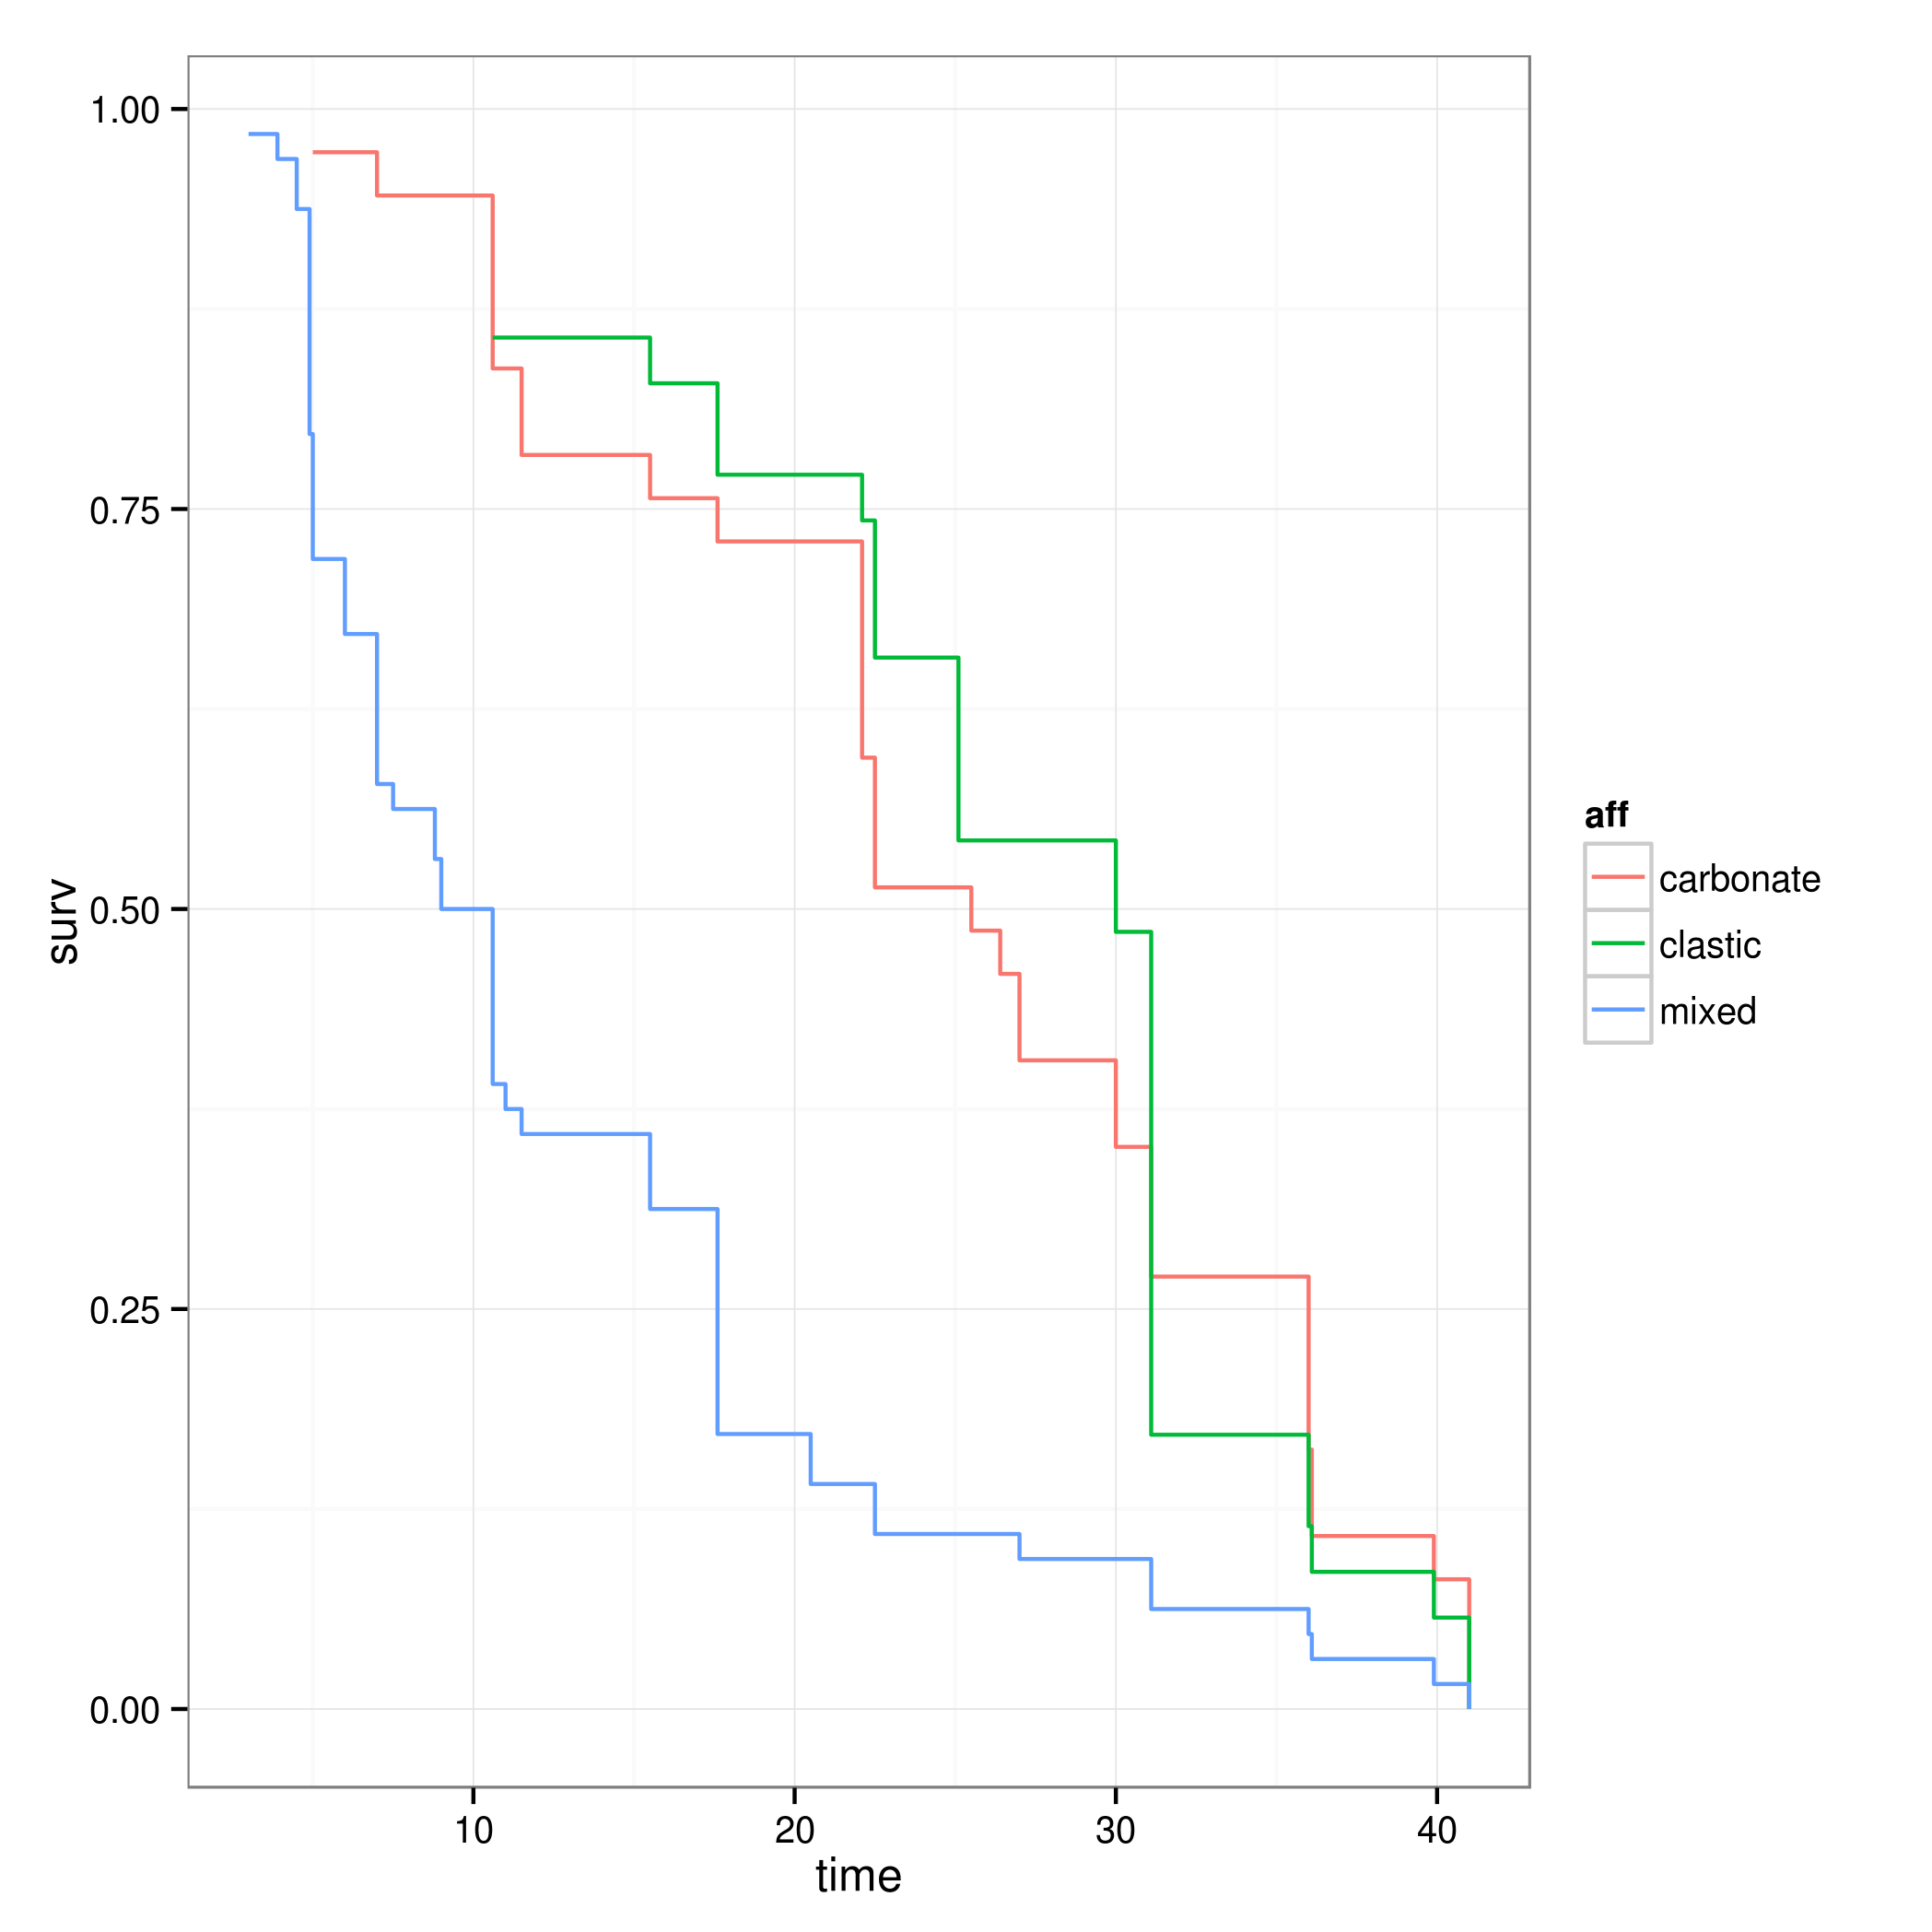
\includegraphics[height = 0.4\textheight, width = \textwidth, keepaspectratio = true]{figure/km_aff}
    \label{subfig:aff_km}
  \end{subfigure}
  \begin{subfigure}[b]{0.5\textwidth}
    \caption{}
    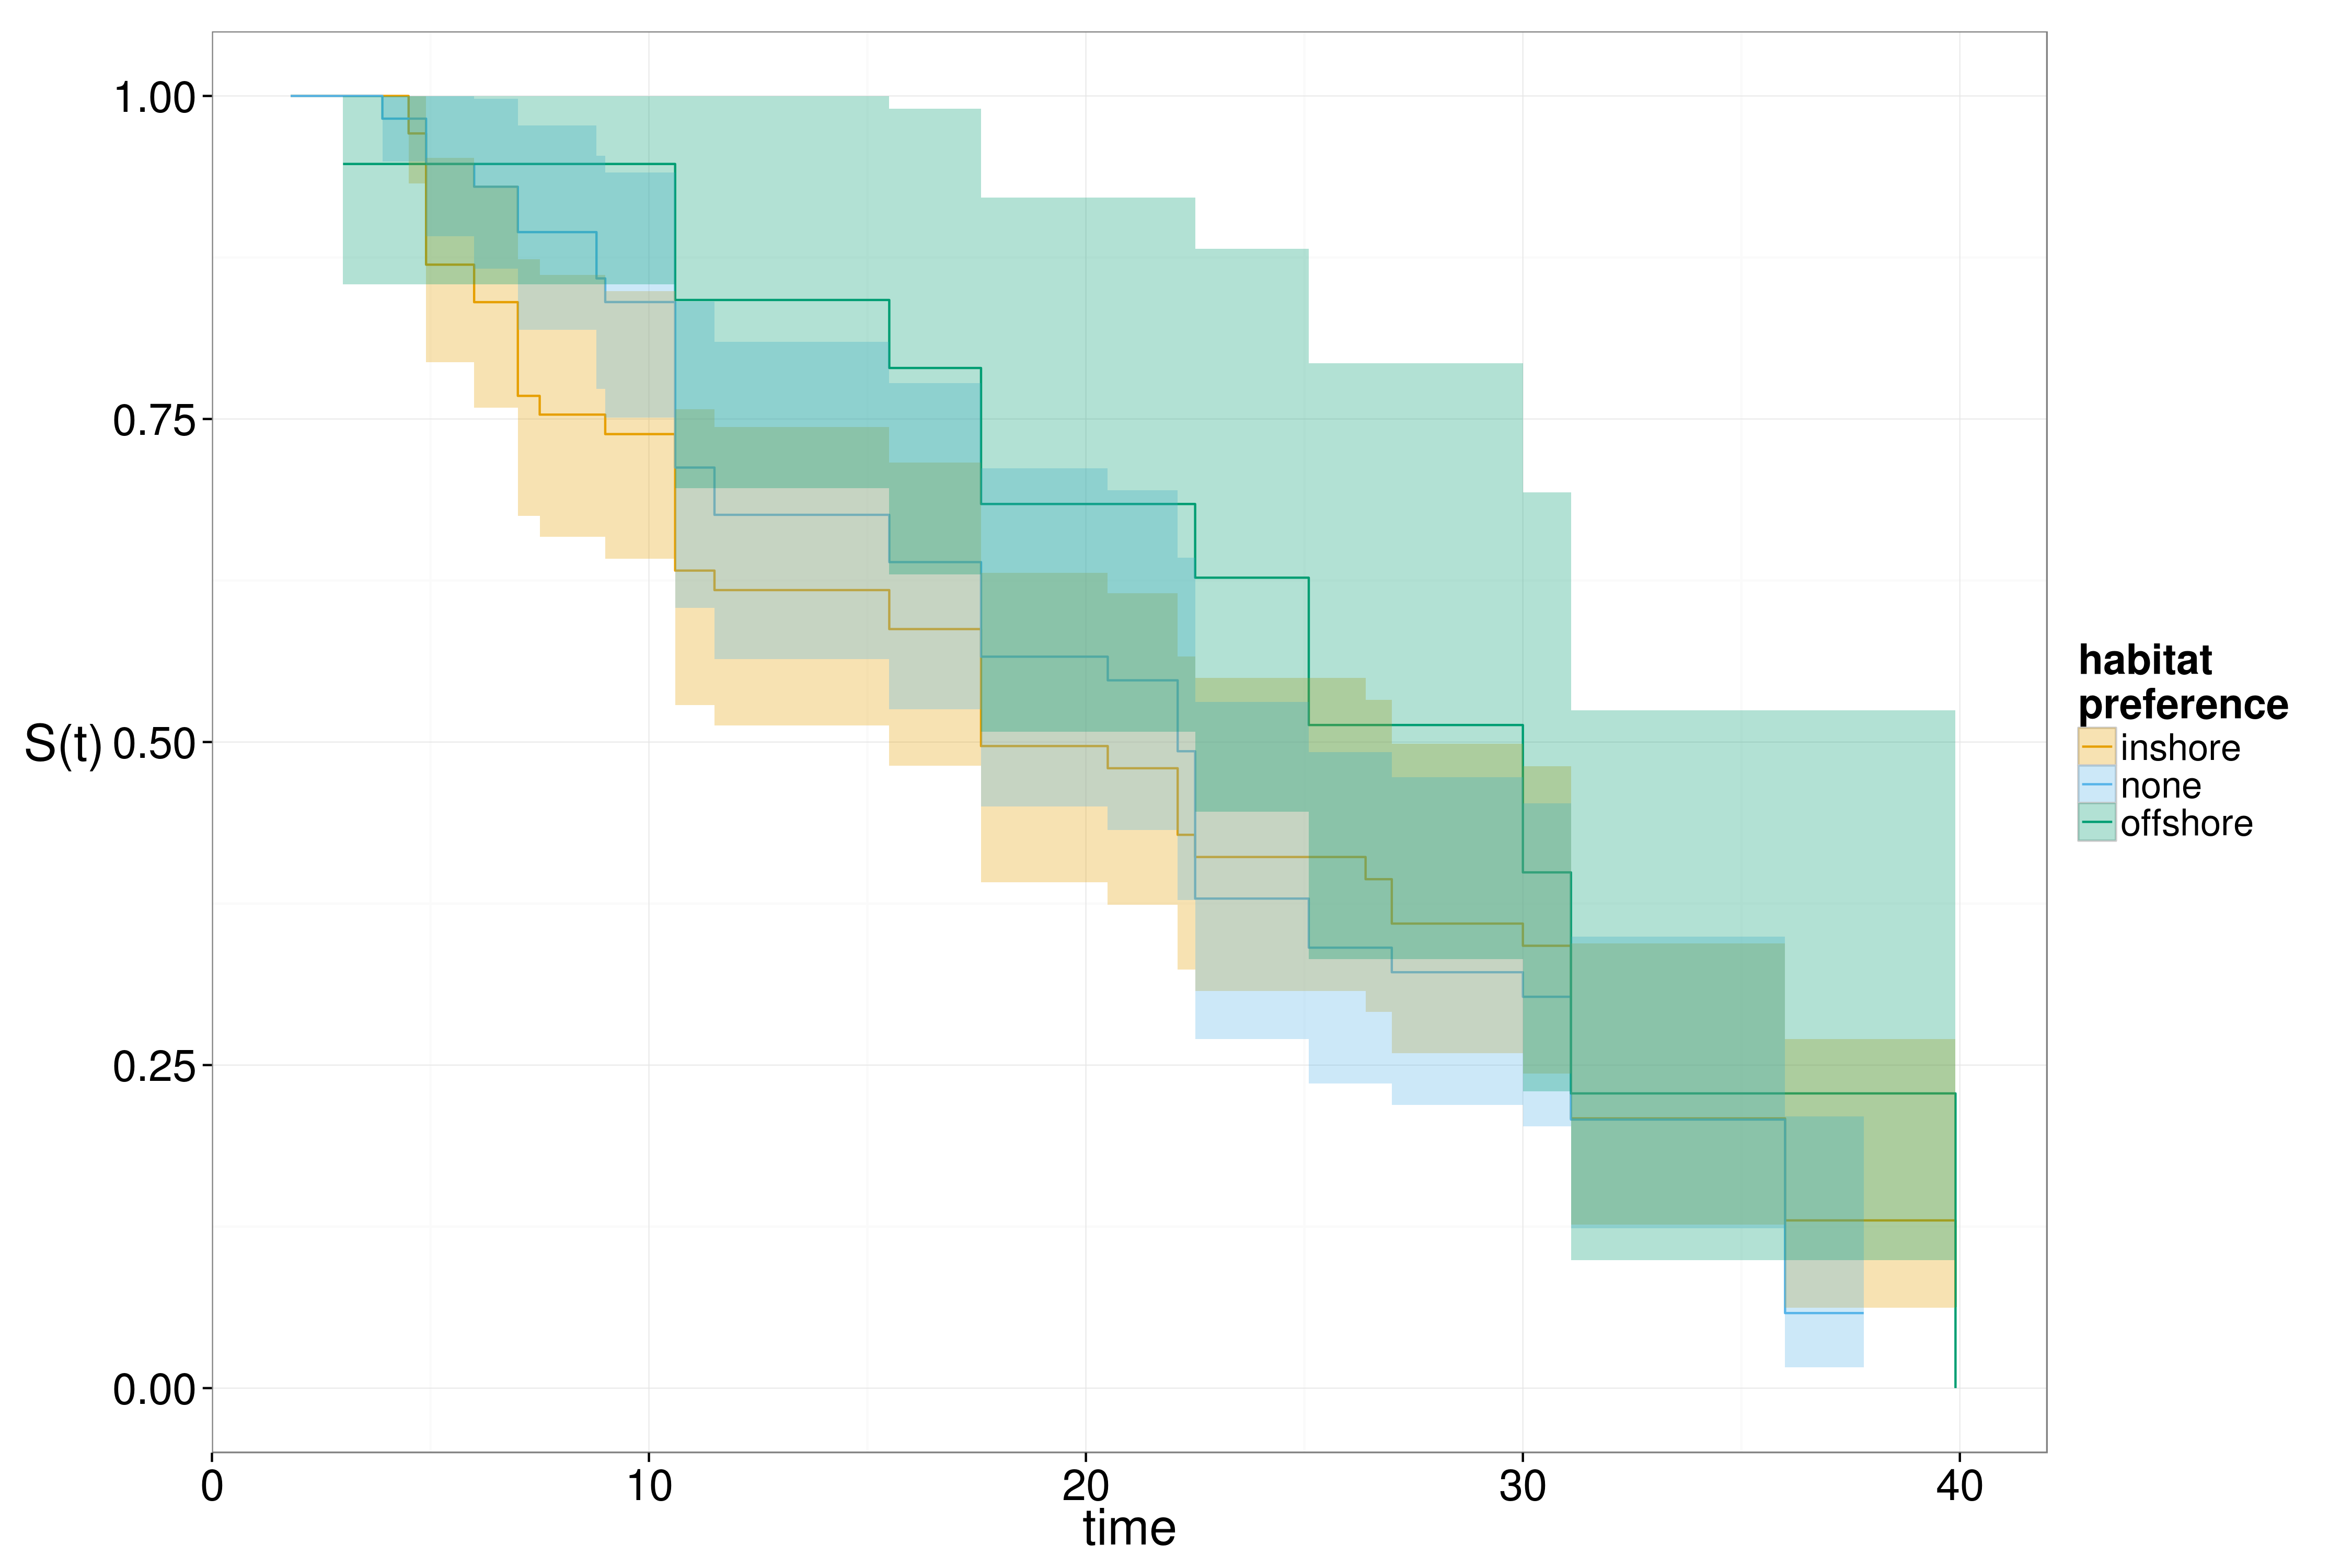
\includegraphics[height = 0.4\textheight, width = \textwidth, keepaspectratio = true]{figure/km_hab}
    \label{subfig:env_km}
  \end{subfigure}

  \begin{subfigure}[b]{0.5\textwidth}
    \caption{}
    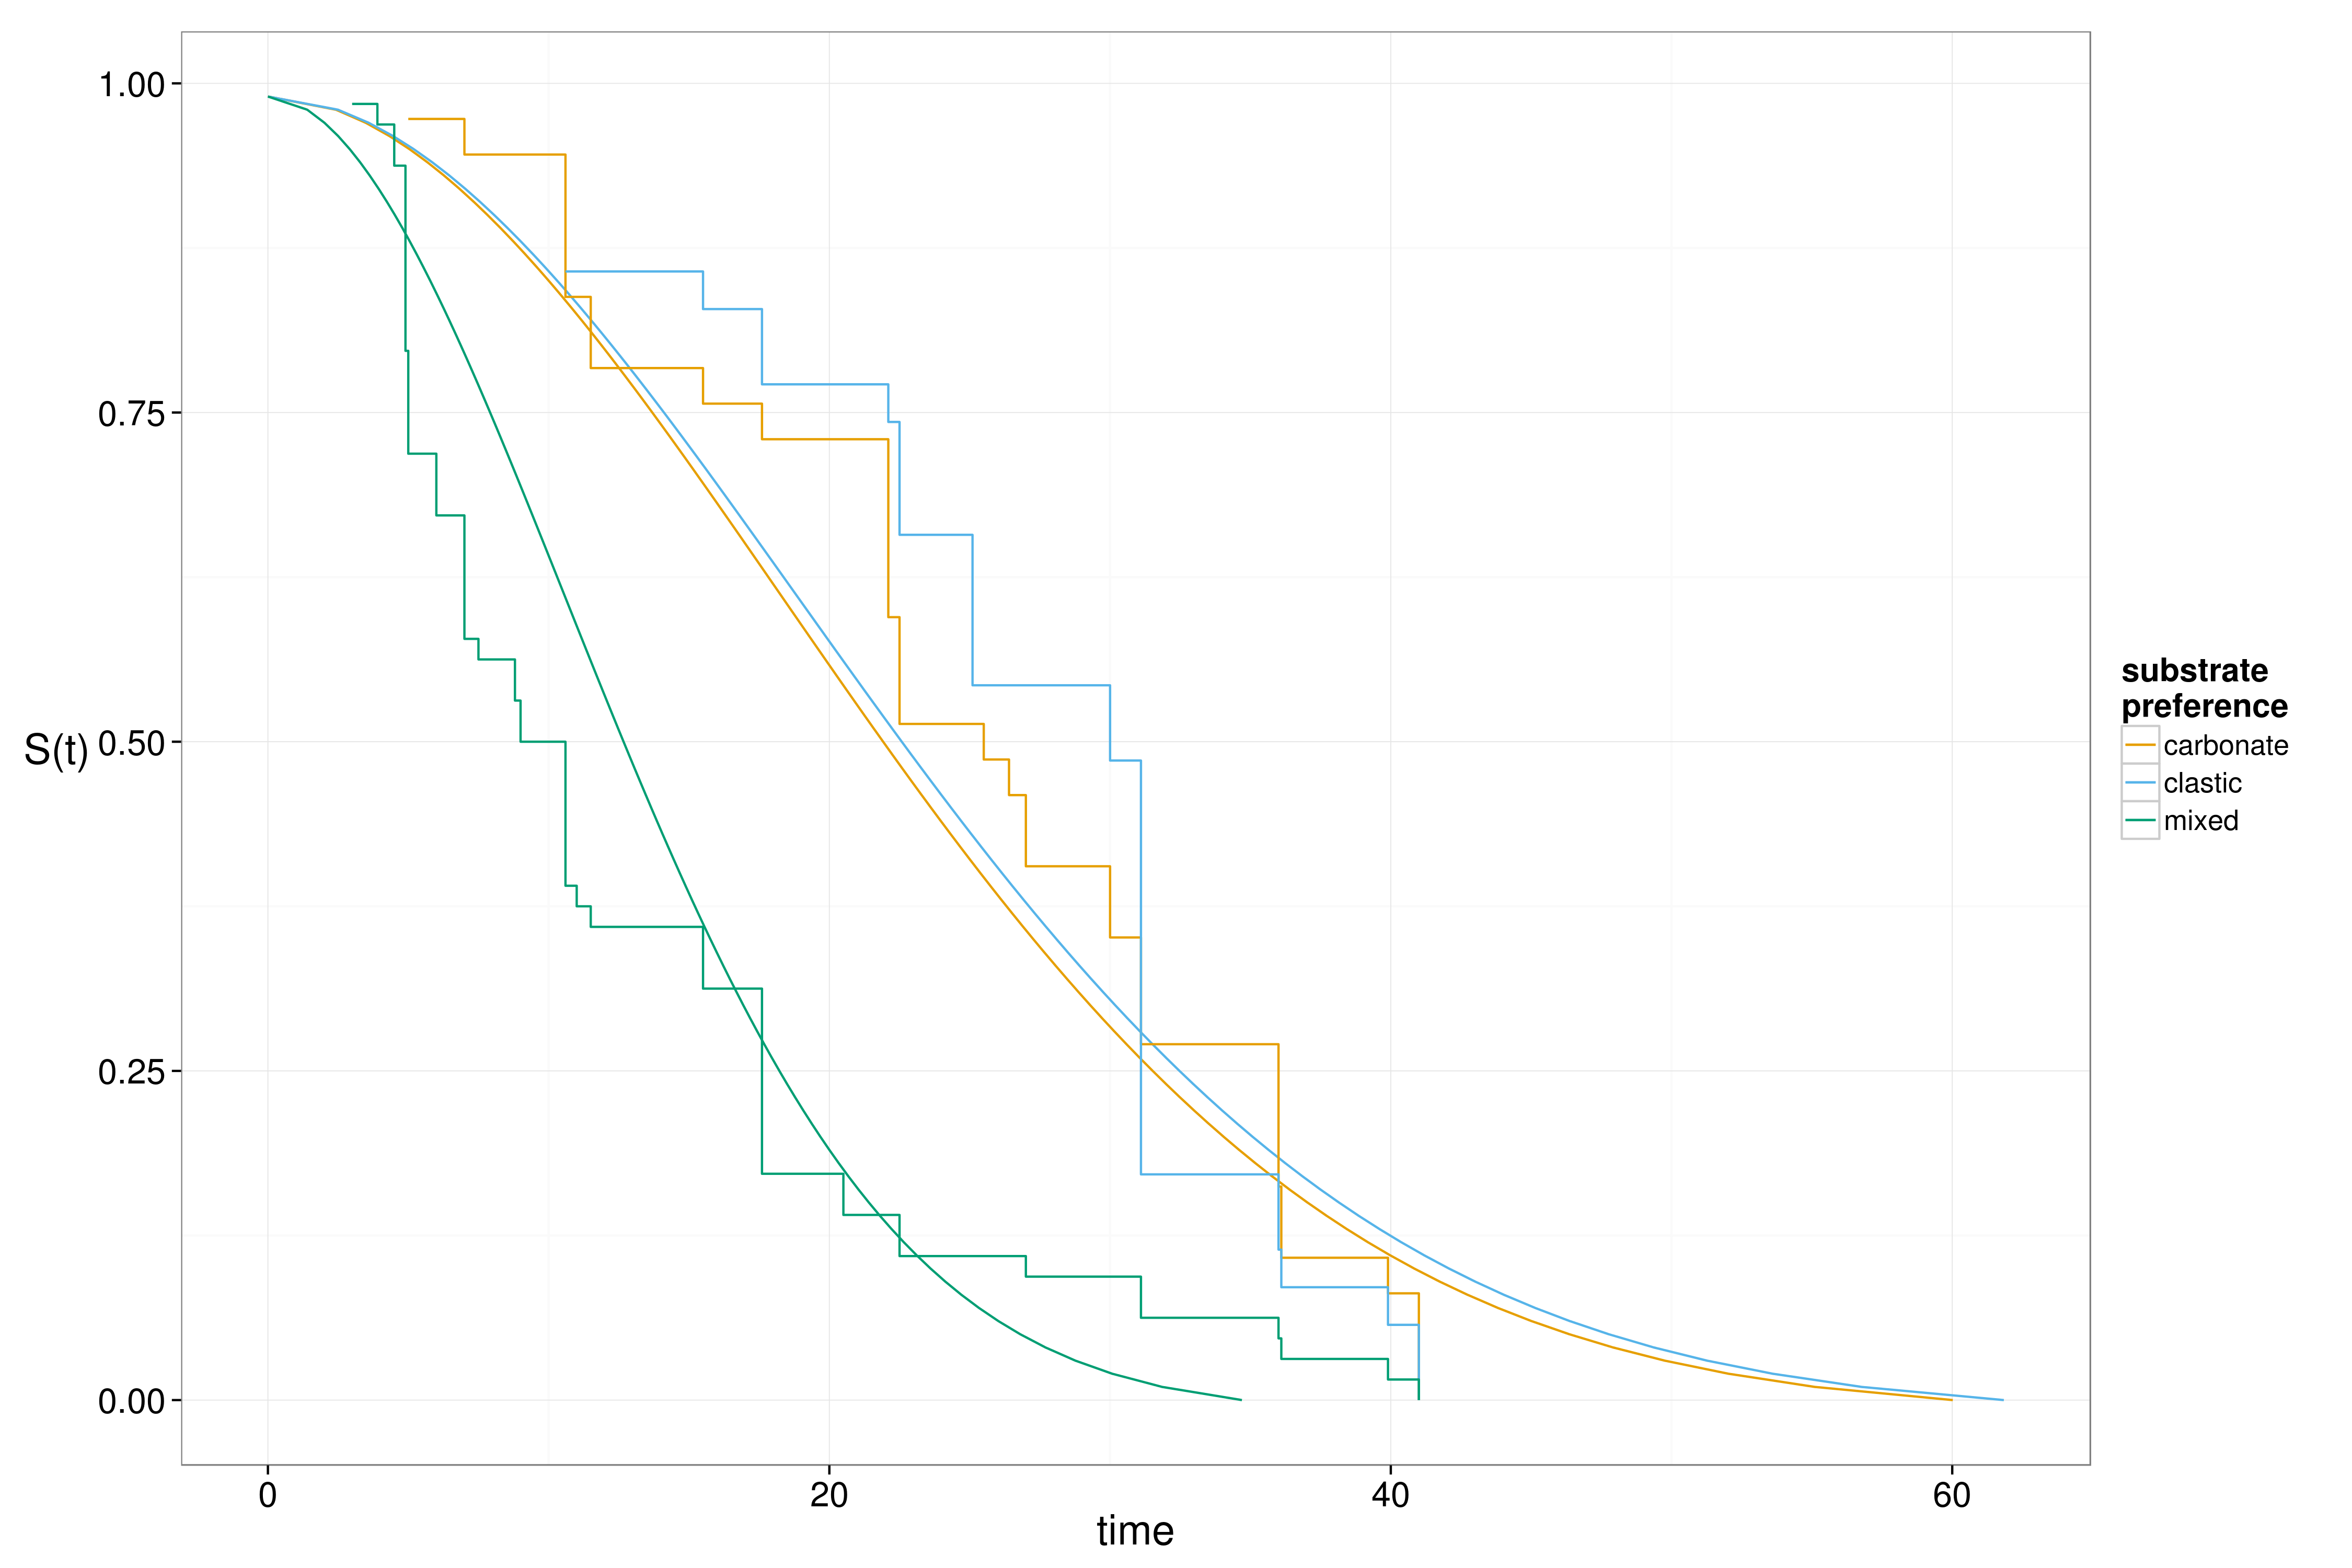
\includegraphics[height = 0.4\textheight, width = \textwidth, keepaspectratio = true]{figure/aff}
    \label{subfig:aff_surv}
  \end{subfigure}
  \begin{subfigure}[b]{0.5\textwidth}
    \caption{}
    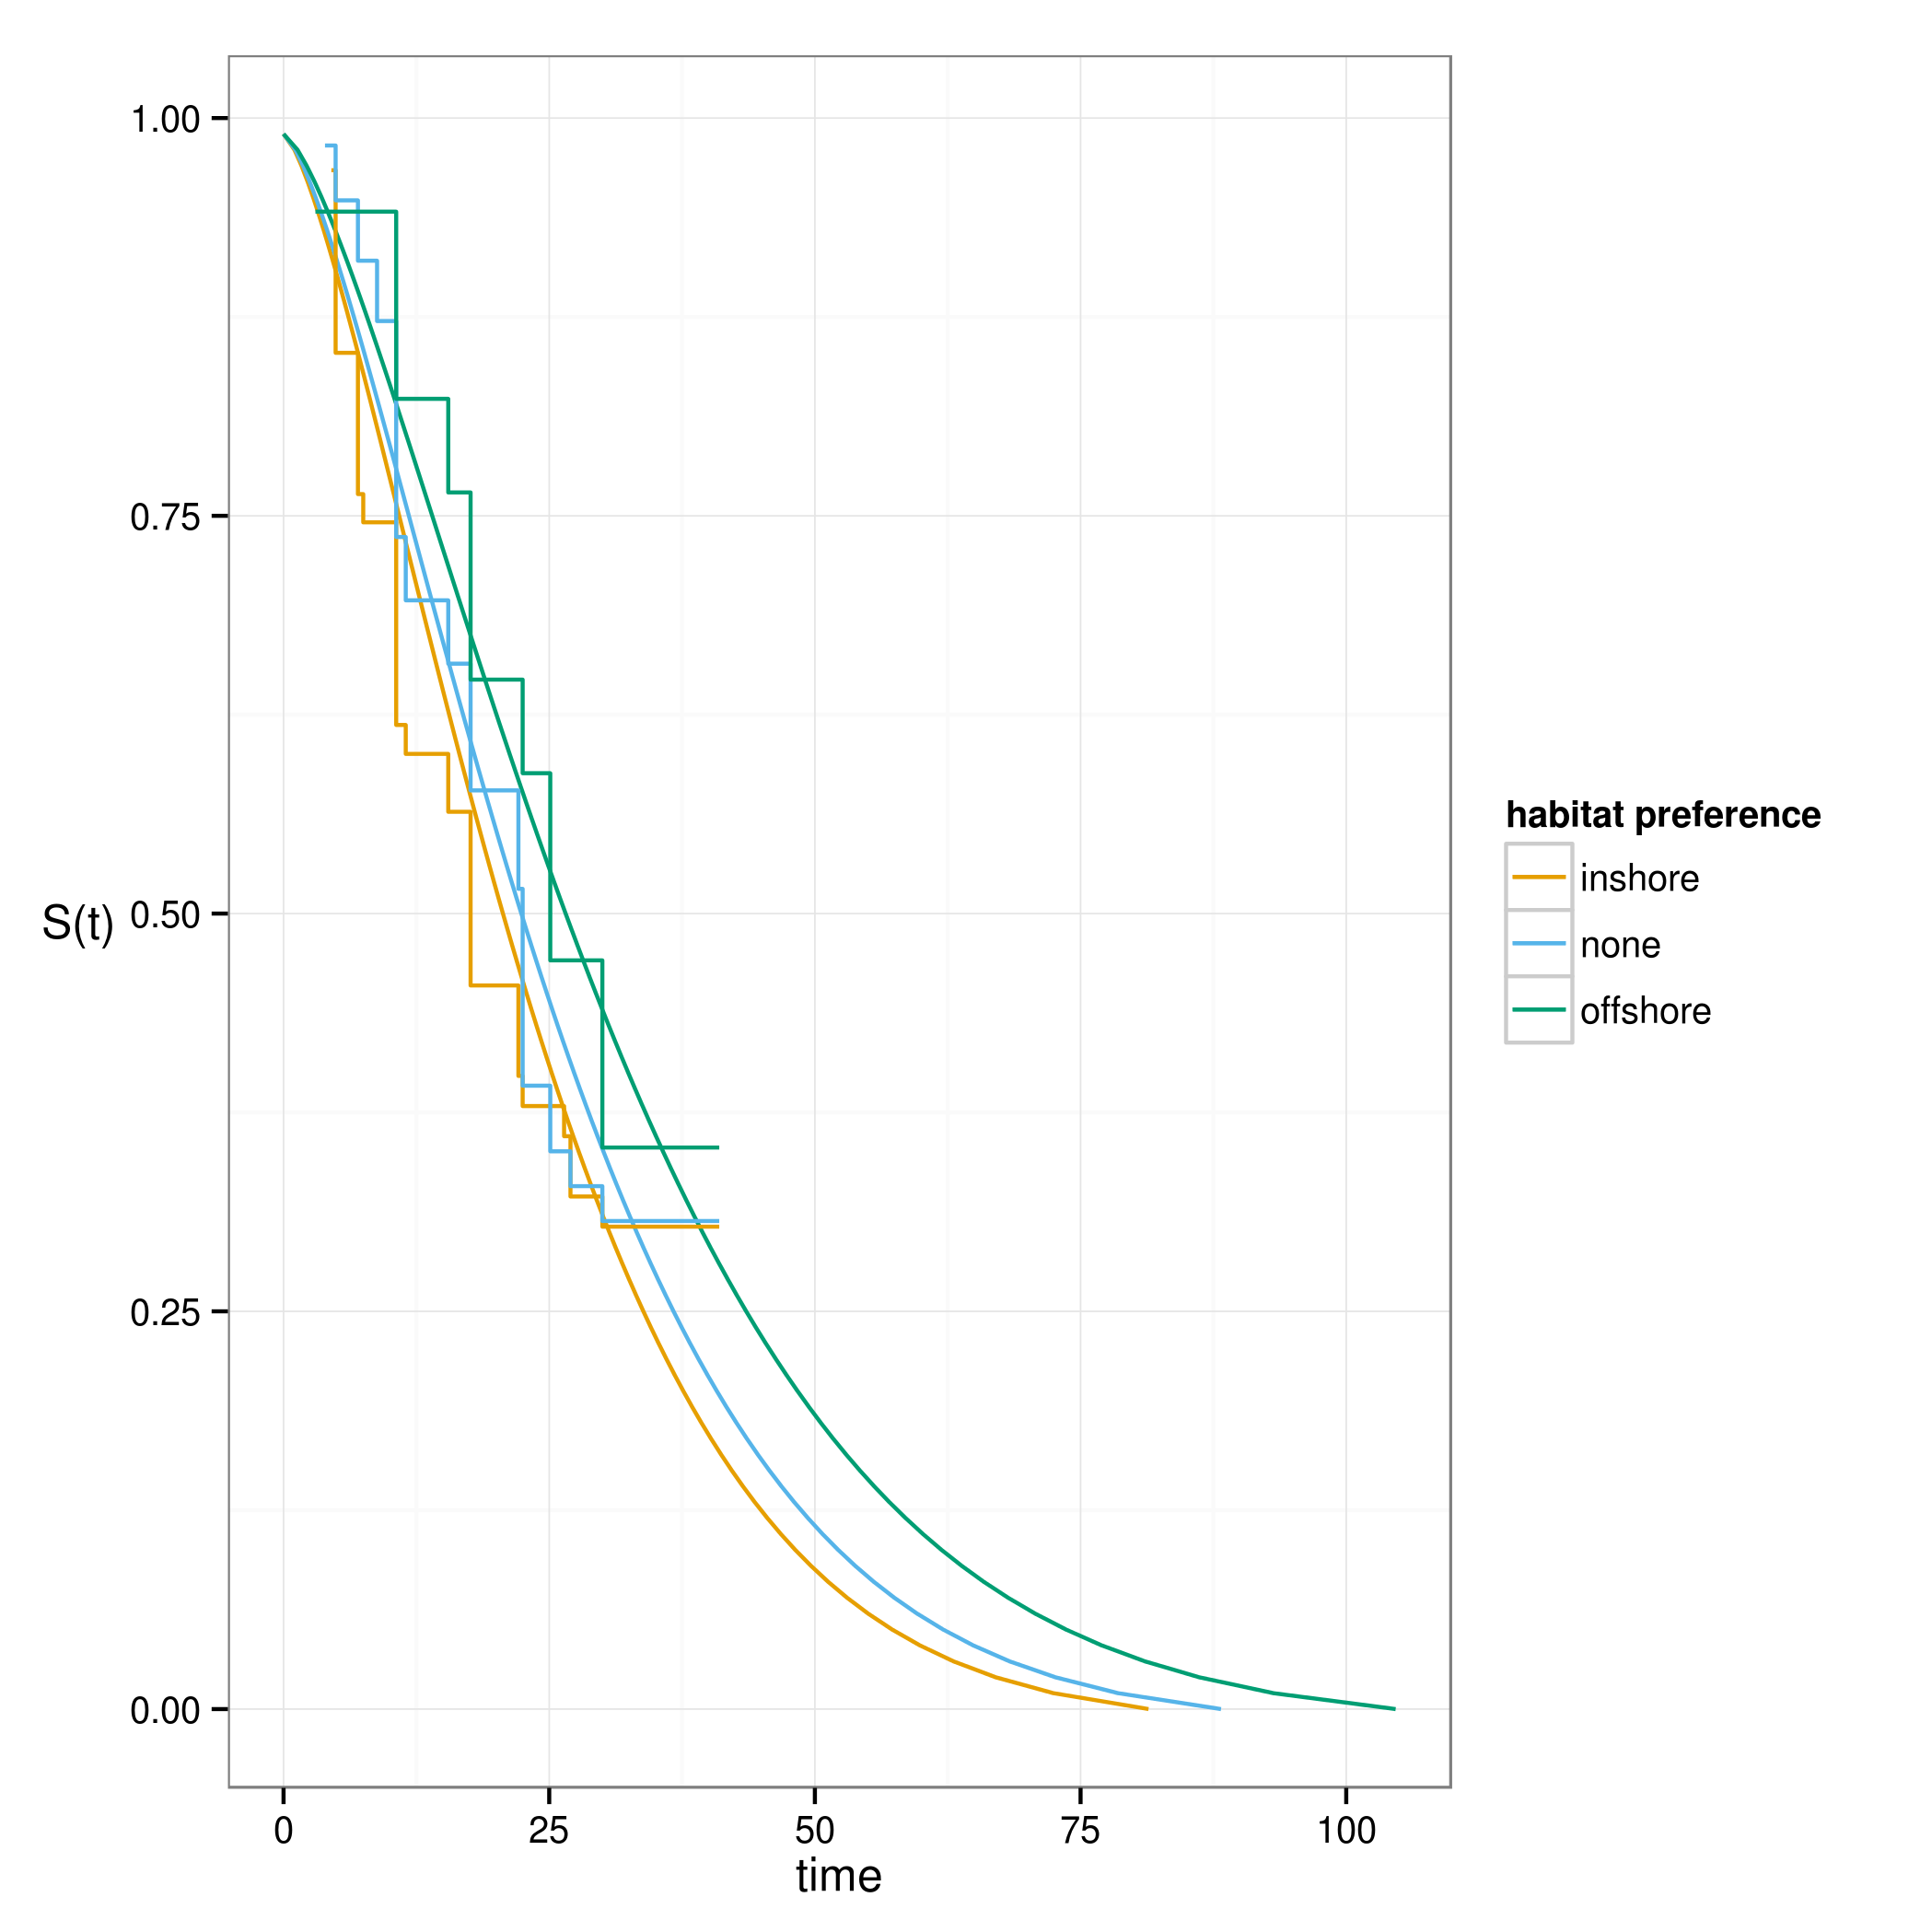
\includegraphics[height = 0.4\textheight, width = \textwidth, keepaspectratio = true]{figure/hab}
    \label{subfig:env_surv}
  \end{subfigure}
  \caption[Brachiopod survival curves]{Survivorship curves of Australian Permian brachiopod genera based on substrate affinity and habitat preference. The stepwise functions are nonparametric Kaplan--Meier survival curves for both substrate affinity (\subref{subfig:aff_km}) and habitat preference (\subref{subfig:env_km}). K-M curves are illustrated with 95\% confidence intervals. The predicted survival curves based on the best parametric models with substrate (\subref{subfig:aff_surv}) and habitat (\subref{subfig:env_surv}) as predictors. The parametric curves are illustrated with the standard errors of prediction.} 
  \label{fig:brach_surv}
\end{figure}

The shape parameter (\(k\)) of the AICc best model (Fig. \ref{subfig:aff_surv}) is estimated to be approximately 1.85 (Table \ref{tab:bracmod}). As described above (Section \ref{sec:surv}), values of \(k\) greater than 1 indicate that failure (extinction) risk accelerates with taxon age, which may mean that the Law of Constant Extinction does not hold when modeling generic level extinction in brachiopods.

For brachiopod survival based on substrate affinity (Fig. \ref{subfig:aff_surv}), survival was greater for both carbonate and clastic affinities and lowest for taxa with mixed affinity. Visual inspection of the estimated survival functions compared to the nonparametric Kaplan--Meier curves indicates that they are adequate fits to the data (Fig. \ref{subfig:aff_km}). 

The model with habitat preference being the sole predictor of survival following a Weibull distribution was a poor estimate, with an approximate \(\Delta\)AICc of 22 between this model and the AICc best model. There is a great degree of deviance between the nonparametric Kaplan--Meier curves and model predictions (Fig. \ref{subfig:env_km}). Additionally, this model is not significantly different from the model with only an intercept (\(\chi^{2} = 1.14\), \(df = 2\), \(p = 0.57\)). This means, preliminarily, that habitat preference alone makes no difference in generic level survival.

Further refinements to these models include modeling survival using other distributions of survival such as a log-normal distribution. Additionally the inclusion of affixing strategy and climate as predictors will increase the understanding of the biology underlying brachiopod generic survival. 

\subsection{Brachiopod distribution and community connectedness} \label{sec:braccom}
\subsubsection{Questions} \label{sec:braccomques}
Given the repeated major glacial activity during the Permian, how stable was community connectedness in Permian brachiopods? Are patterns of community connectedness different for taxa favoring different environments?

\subsubsection{Hypotheses and predictions} \label{sec:braccompred}
During the Permian, the east coast of the Australian continent faced towards the massive Panthalassic Ocean. Because of this, the establishment of populations was most likely limited to within the local area because the amount of distance required to establish else was most likely too great. Additionally, individuals which settled across the ocean would have been almost instantly genetically isolated and not increase community connectedness, \textit{per se}. Because of this, it is expected that community connectedness in Australian Permian brachiopods would be fairly high at any given time and that changes, specifically decreases in connectedness, would be expected during the four glacial periods \citep{Fielding2008a,Fielding2008}.

Dispersal ability of modern brachiopods appears to be most limited by availability and proximity of substrate types \citep{Richardson1997,Richardson1997a}. The Permian of Australia is dominated by widespread clastic beds compared to relatively few carbonate beds. The expectation is that the distribution of taxa with a carbonate preference will be extremely patchy with a high \(E\) (Eq. \ref{eq:e}), low \(Occ\) (Eq. \ref{eq:occ}), low \(BC\) (Eq. \ref{eq:bc}), and low code length \citep{Rosvall2008,Sidor2013} compared to the distribution of clastic preferring taxa. However, if community connectedness is approximately equal between carbonate and clastic preferring taxa this could be caused by approximately equal dispersal ability in both groups, either high or low.

Habitat would be expected to influence community structure if there is an uneven distribution of available habitats in space and time. Rarity of preferred habitat would be expected to lead to high \(E\), low \(Occ\), low \(BC\), and low code length compared to an abundance of preferred habitat. Because of the four major glaciation events during the Permian of Australia, it is expected that the availability of on-shore habitats would be highly variable. It is then expected that during periods of glacial activity community connectedness of on-shore preferring taxa would be extremely low because of rarity of environments in comparison to both periods of non-glacial activity and off-shore habitats at all times. If habitat preference has no effect on community connectedness this may mean that the dispersal ability of on-shore taxa is very high and able to maintain gene flow between potentially isolated habitats.

It is expected that affixing strategy alone will have minimal effect on community connectedness unless affixing strategy is highly correlated with substrate and/or habitat preference. If community connectedness is found to be different between affixing strategies but affixing strategy is not highly correlated with substrate or habitat preference this may be because of spatial heterogeneity in energy levels which limits reclining versus fixed taxon distributions. This scenario is highly unlikely given knowledge of modern and fossil brachiopod distributions \citep{Rudwick1970,Richardson1997,Richardson1997a}.

\subsubsection{Proposed research} \label{sec:braccommeth}
Using a biogeographic network approach (Section \ref{sec:bionet}), I will construct networks between brachiopod genera and localities defined as 2x2 latitude--longitude grid cells from an equal-area map projection. Biogeographic networks will be constructed for the entire Permian using 2 My bins. In addition to community wide networks, separate networks will be constructed for taxa within ecological categories. This facilitates comparison of community connectedness patterns during the Permian both within and between categories as well as with the community wide pattern. The data necessary to complete this study is the same as for the above analysis of brachiopod survival (Section \ref{sec:bracsurv}). Importantly, sampling will be restricted to the east coast of Australia because this represents a continuous coast line that faced the Panthalassic Ocean during the Permian.

Trait assignment will follow the procedure outlined for analysis of brachiopod survival (Section \ref{sec:bracsurvmeth}).

The next step is to compare patterns of community connectedness both within and between regions in order to understand if global, regional, or local scale processes dominate. Additionally, comparisons will be done between the different ecological traits both within and between regions to determine which scale processes may be dominate. The approach and methodology to accomplish these analyses is currently under development. Additionally, the possibility of integrating locality--locality distance or some other measure of topology will be explored, especially how this relates to code length and provinciality in general.

\subsubsection{Preliminary results} \label{sec:braccomres}
Preliminary results are based soley on the brachiopod occurrence information in the PBDB. Preliminary networks were constructed with taxa being defined as genera and locatlies defined from sa 2x2 latitude-longitude grid from an equal area map projection. All localities were restricted to those occurring in basins not present in the state of Western Australia. Networks were also constructed for taxa divided by substrate and habitat preferences. No initial comparisons with the Permian glacial record have been made. These results are based on the lithological and paleoenvironmental data present in the PBDB which will be improved as discussed above (Section \ref{sec:braccommeth}).

\begin{figure}[ht]
  \begin{center}
    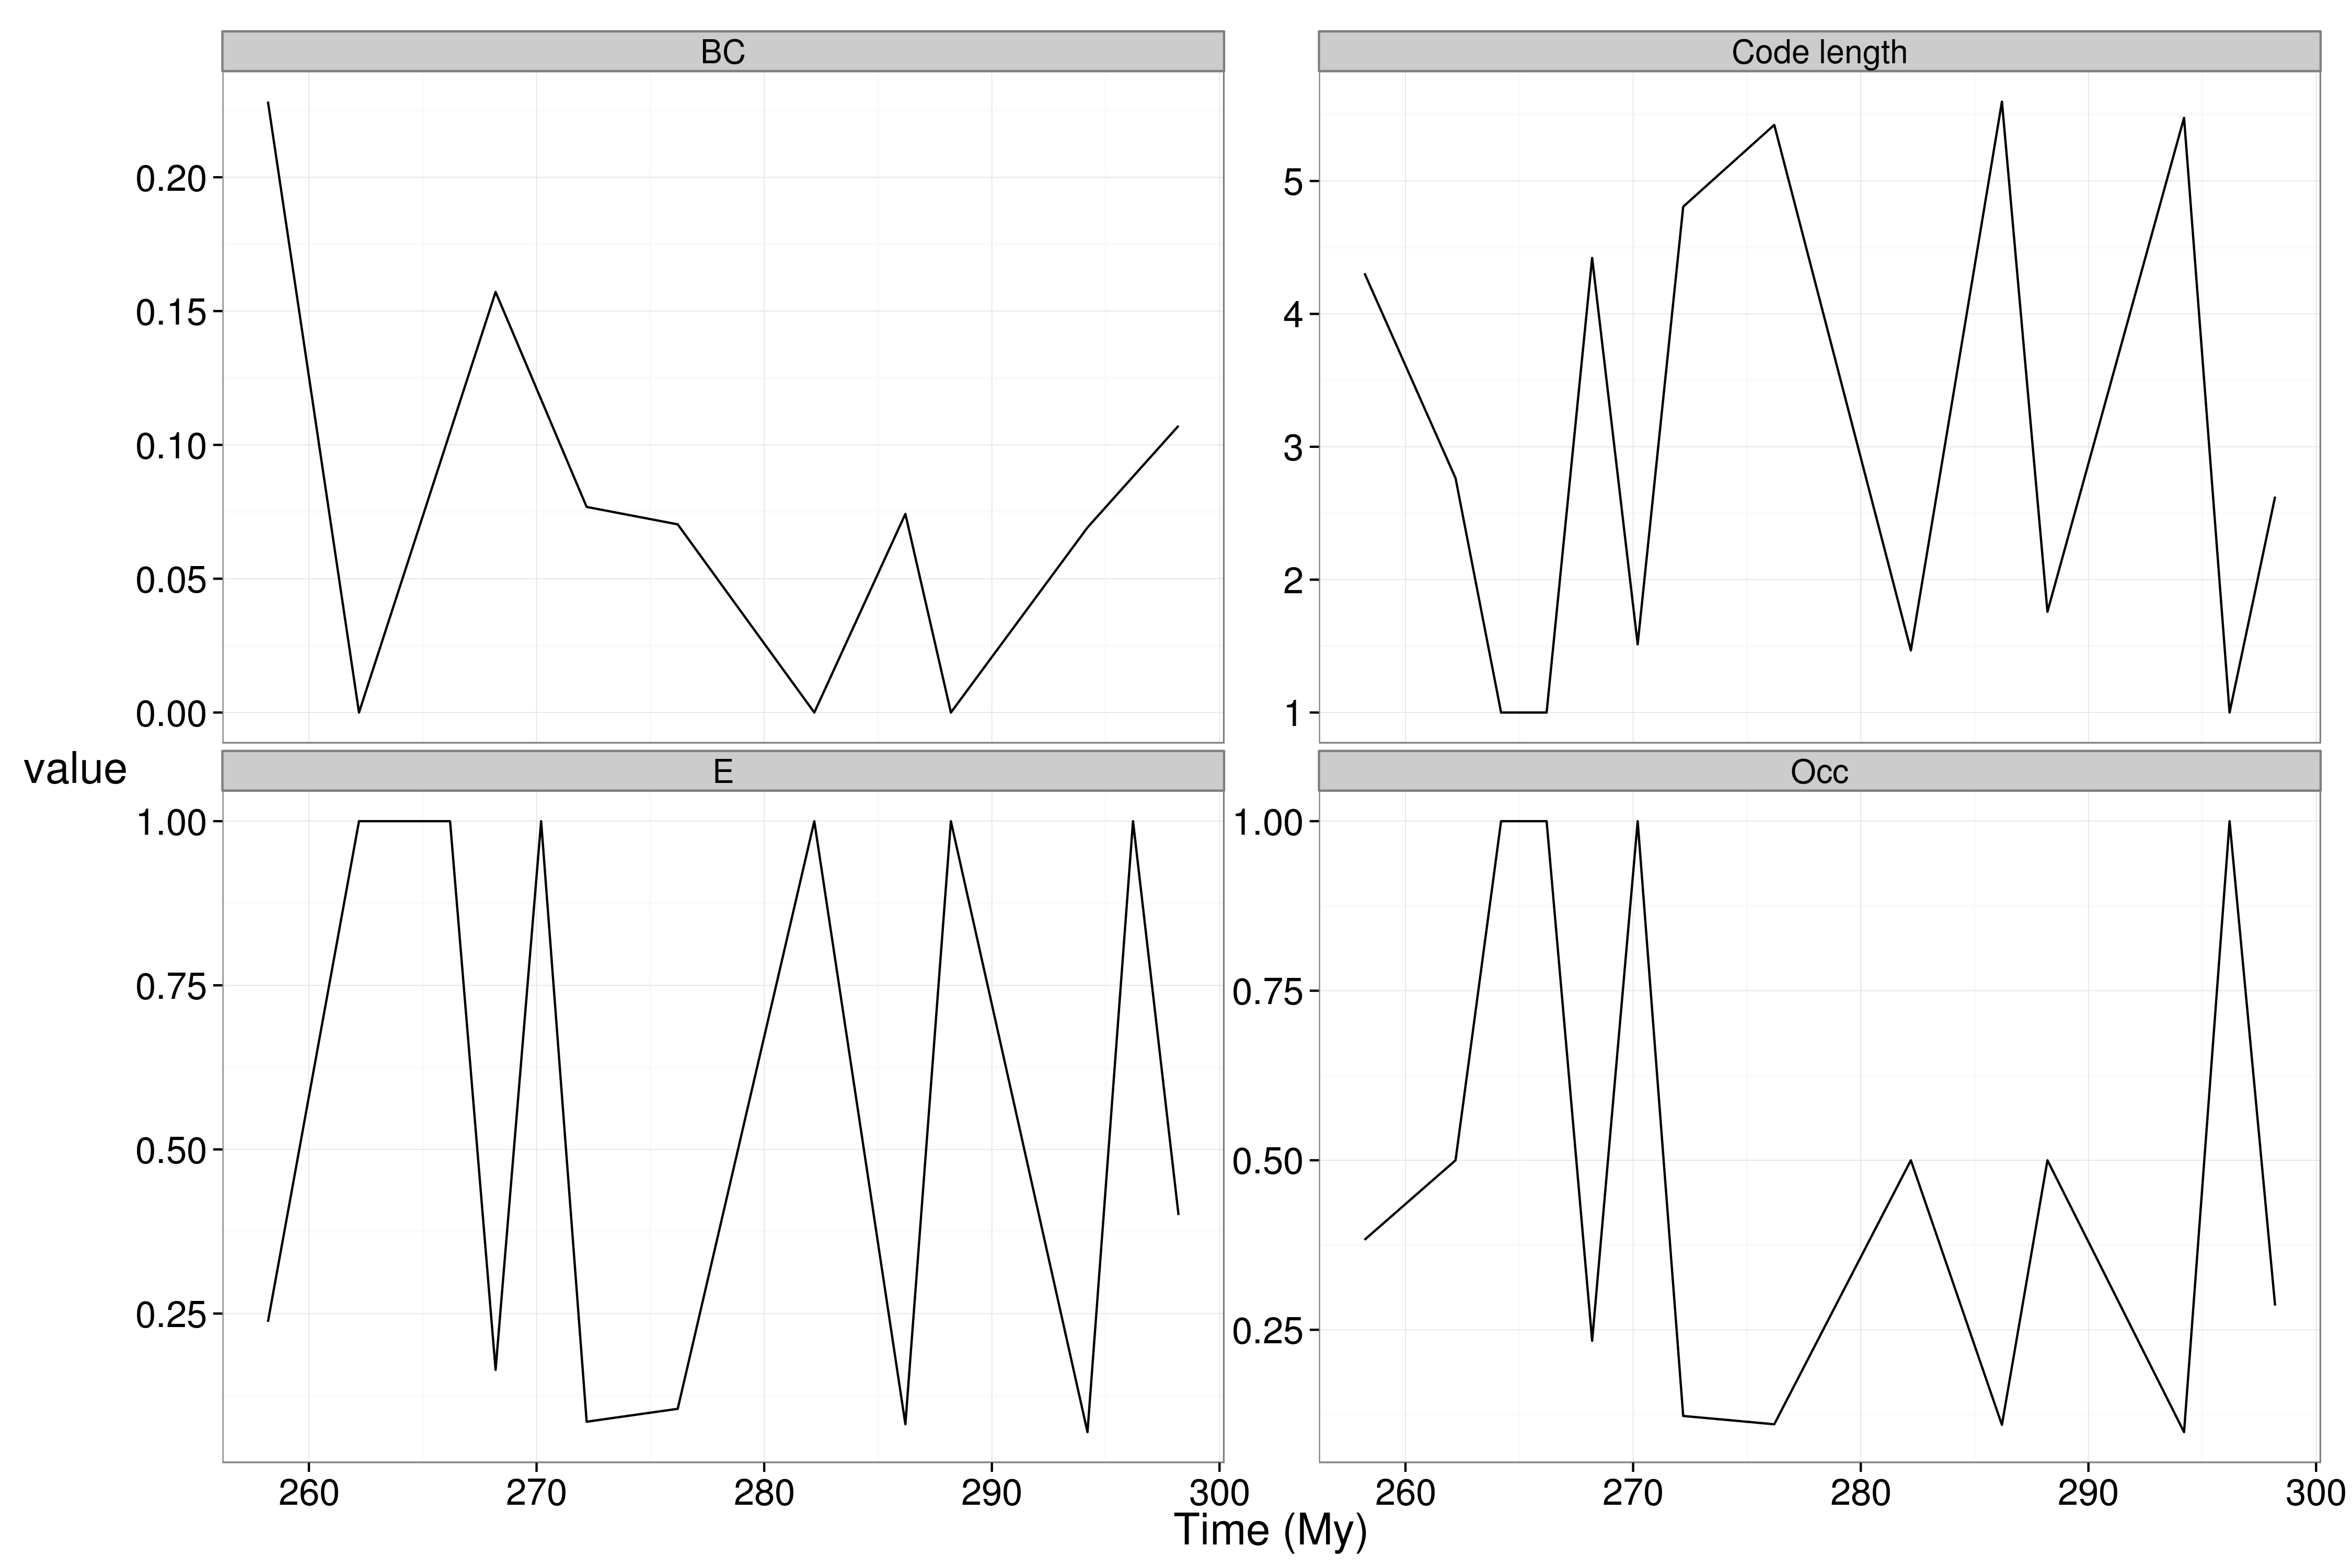
\includegraphics[width = \textwidth, keepaspectratio = true]{figure/east_cast}
  \end{center}
  \caption[Community connectedness statistics for Australaian brachiopods]{Summary statistics of community connectedness for all brachiopods occurring on the East coast of Australia during the Permian. The summary statistics are, clockwise from top left: biogeographic connectedness (BC), code length, average relative locality occupancy per taxon (Occ), and average relative number of endemic taxa per locality (E).} 
  \label{fig:brac_net}
\end{figure}

The summary statistics for community connectedness for all brachiopods show a qualitatively random pattern (Fig. \ref{fig:brac_net}) with no observable trends. Three of four summary statistics fluctuate continually (\(E\), \(Occ\), code length) while \(BC\) is qualitatively stationary throughout the Permian. Importantly, this pattern is effectively the same as that seen in clastic preferring taxa (Fig. \ref{subfig:sub_net}). These preliminary results are also demonstrate the predicted rarity of carbonate preferring taxa (Fig. \ref{subfig:sub_net})

Additionally, taxa with both in-shore and no habitat preference have approximately identical patterns that are also qualitatively random in contrast to the qualitatively stable off-shore preferring taxa (Fig. \ref{subfig:hab_net}). 

\begin{figure}[ht]
  \begin{center}
    \begin{subfigure}[b]{0.4\textwidth}
      \caption{}
      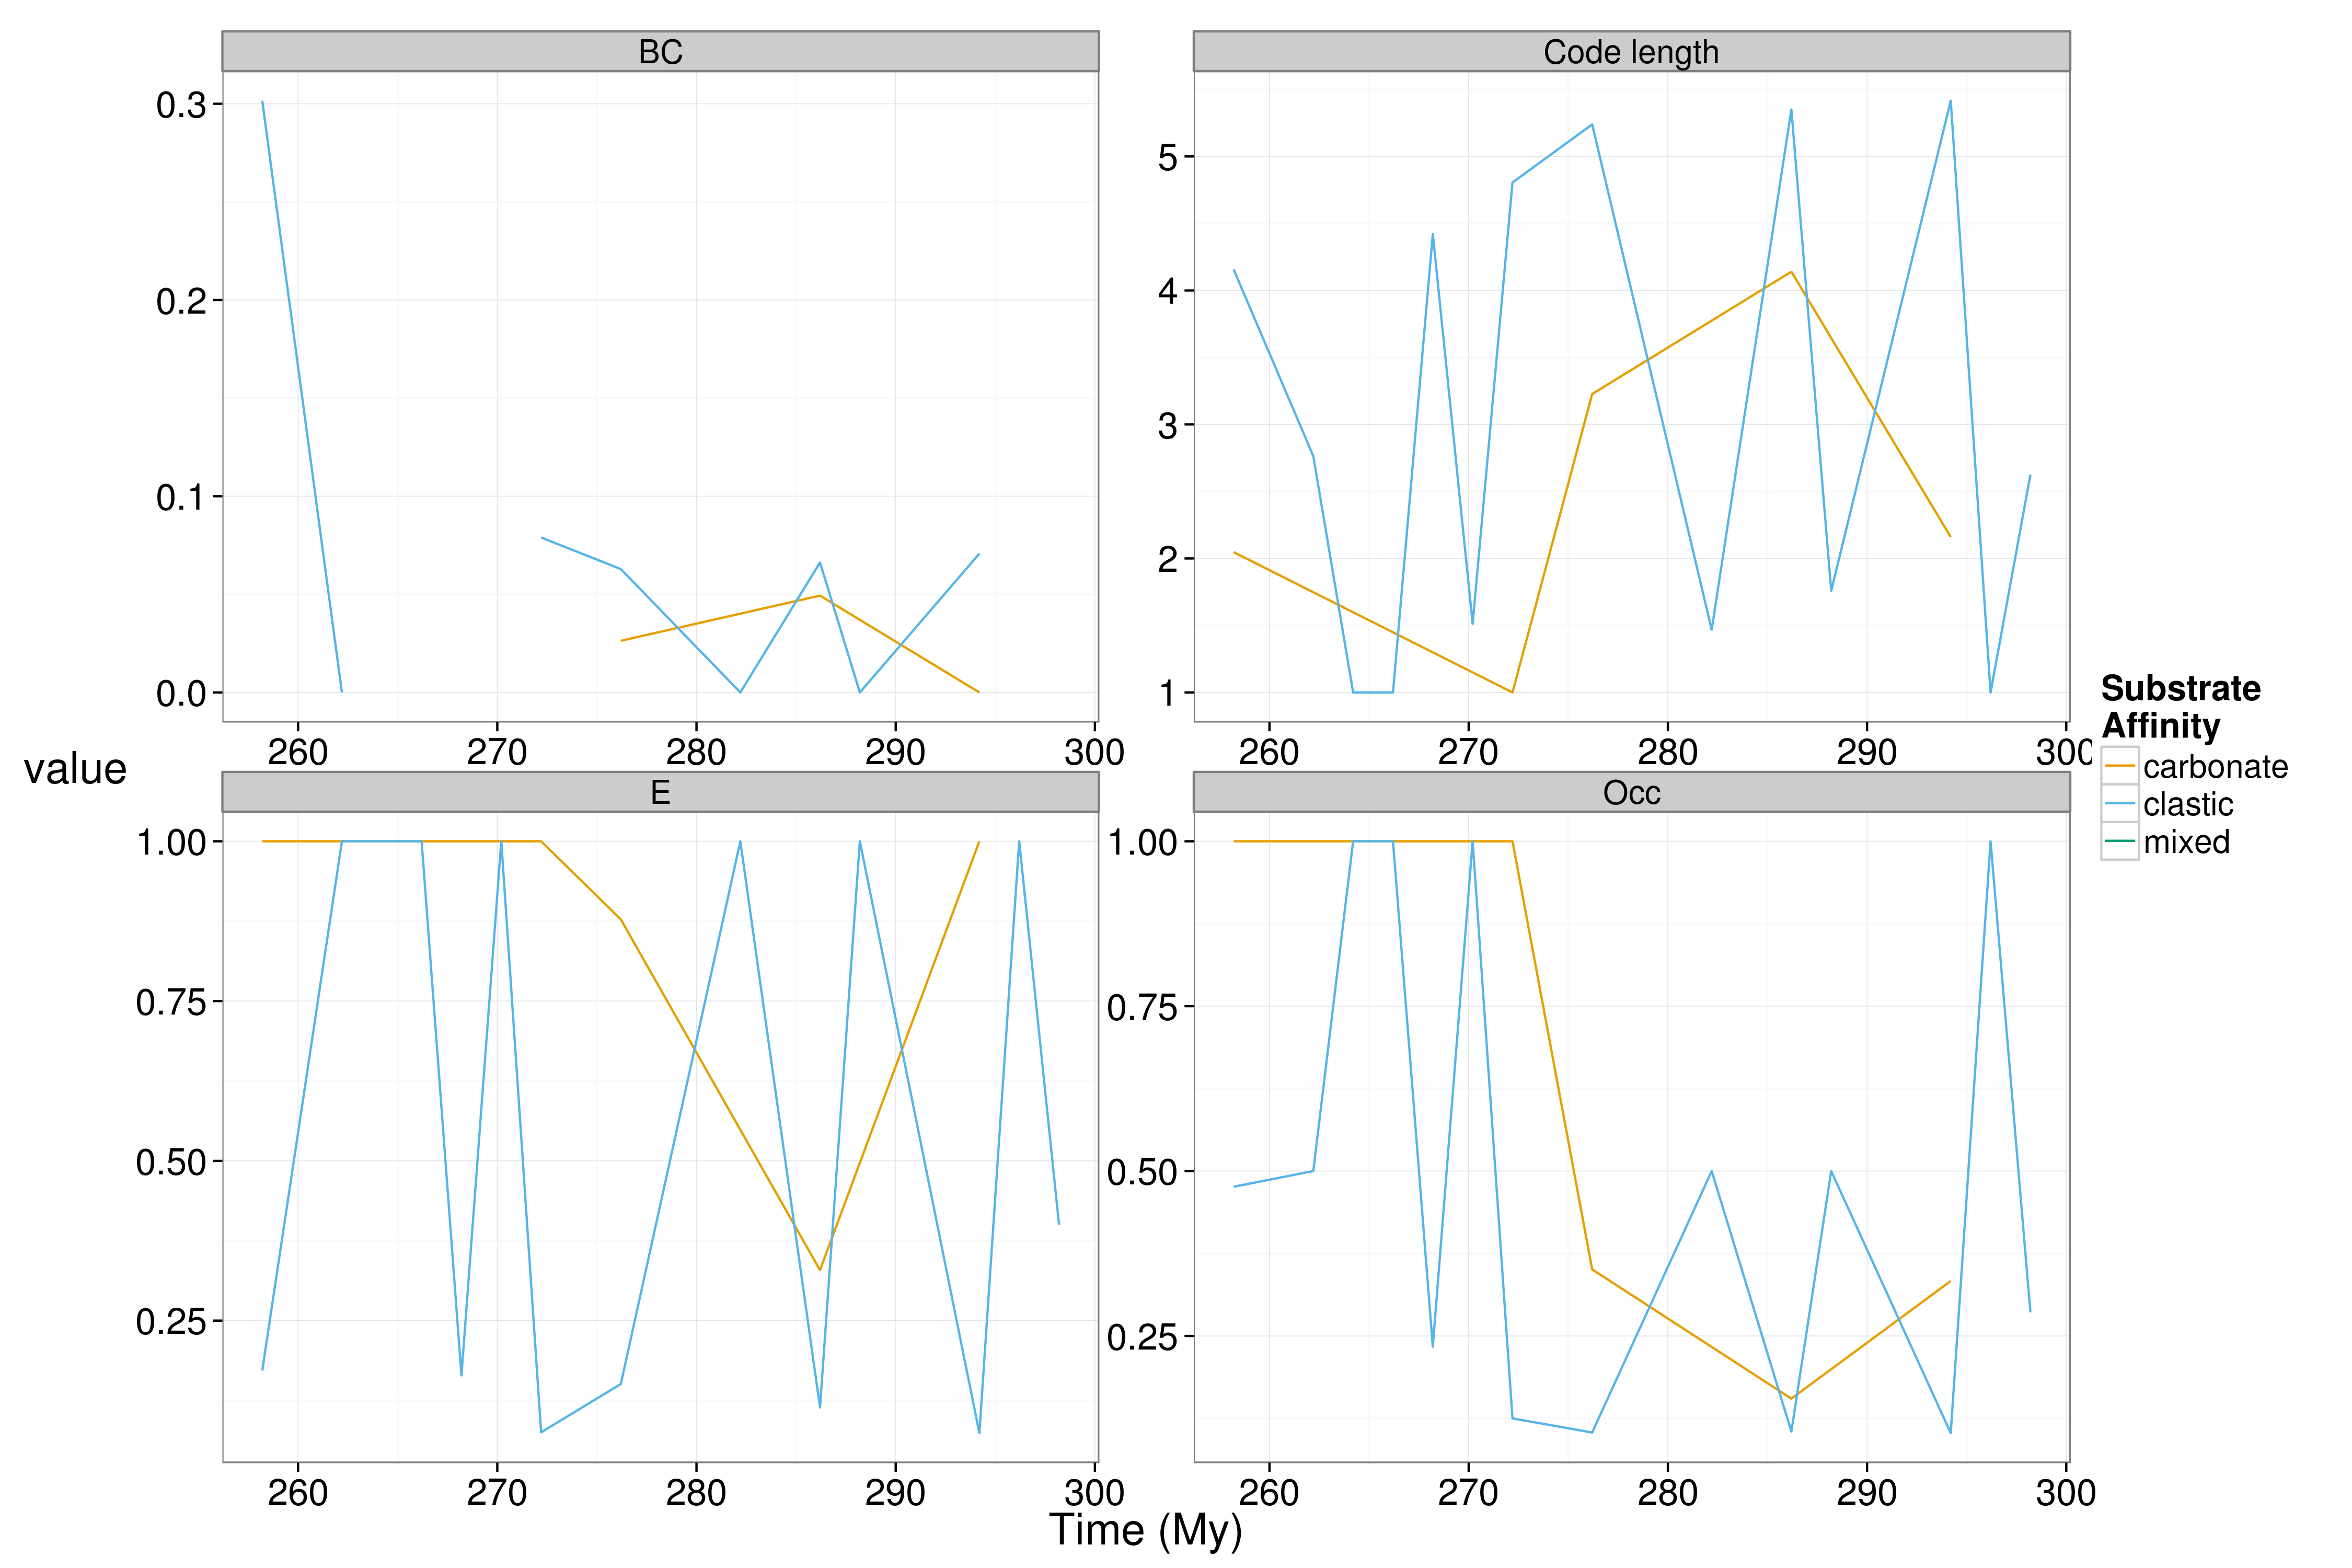
\includegraphics[width = \textwidth, keepaspectratio = true]{figure/substrate_network}
      \label{subfig:sub_net}
    \end{subfigure}
    \begin{subfigure}[b]{0.4\textwidth}
      \caption{}
      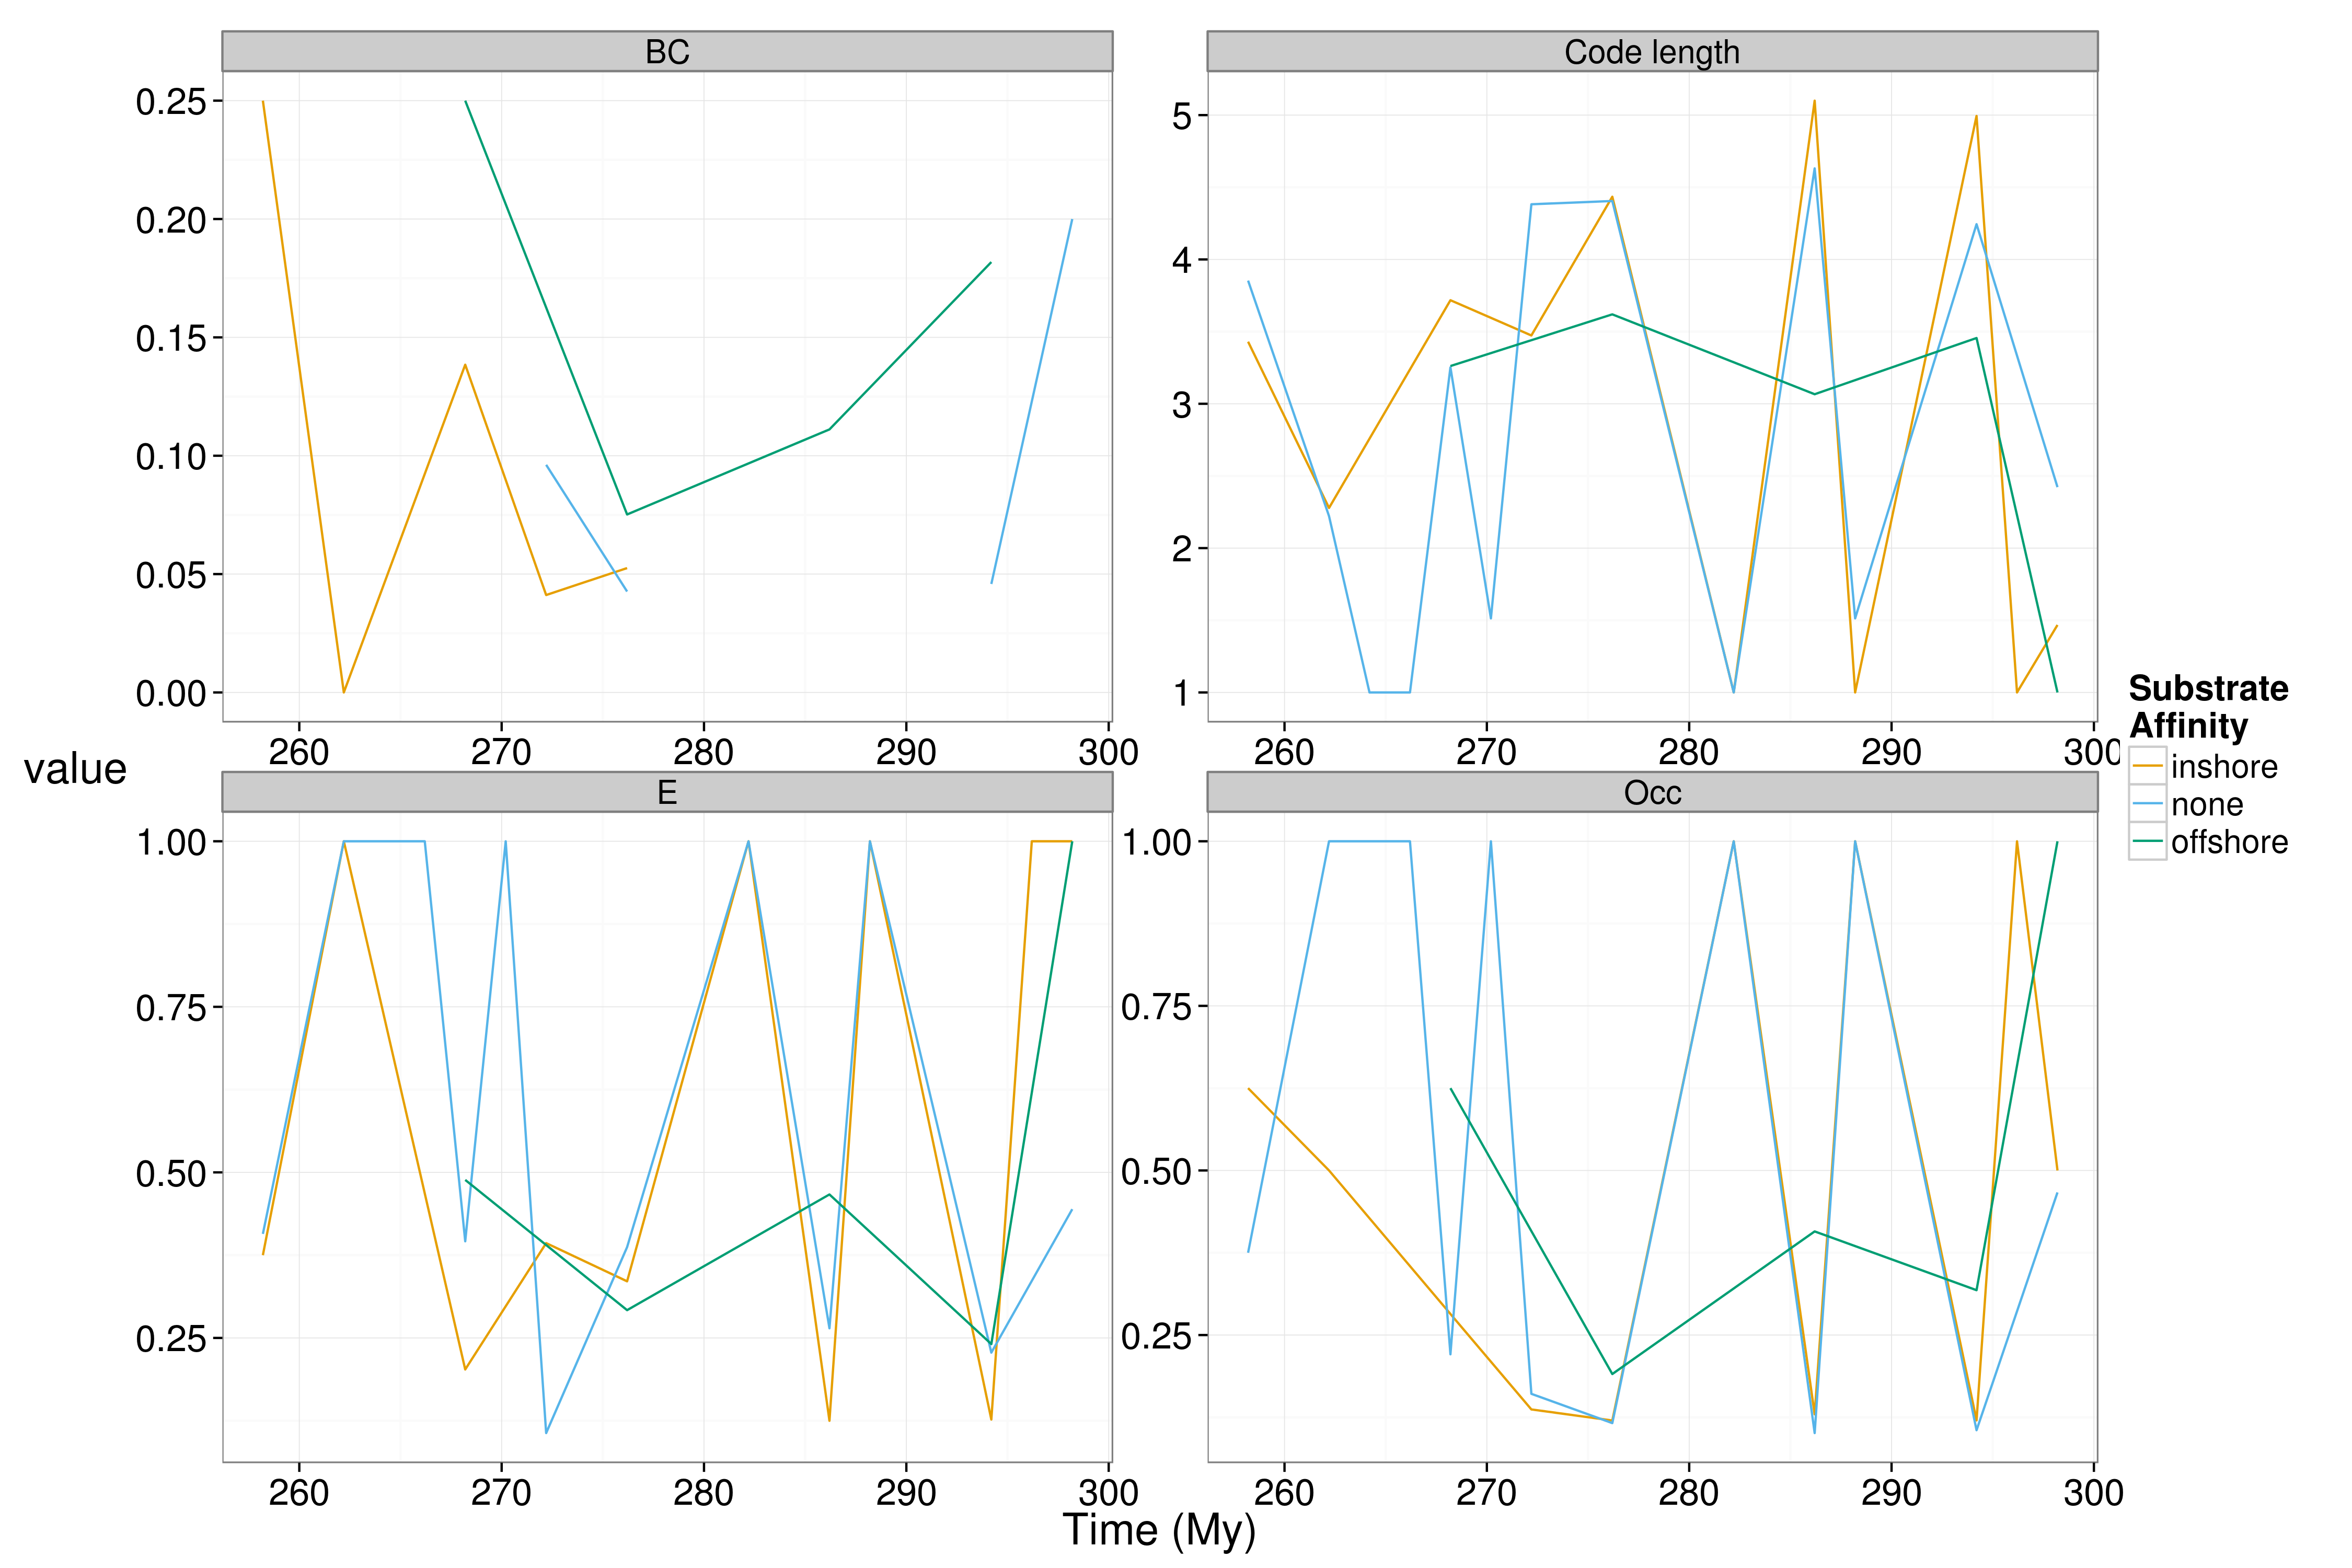
\includegraphics[width = \textwidth, keepaspectratio = true]{figure/habitat_network}
      \label{subfig:hab_net}
    \end{subfigure}
  \end{center}
  \caption[Trait based brachiopod community connectedness summary statistics]{Community connectedness statistics for brachiopods separated by substrate (\subref{subfig:sub_net}) and habitat (\subref{subfig:hab_net}) preference. The summary statistics are, clockwise from top left: biogeographic connectedness (BC), code length, average relative locality occupancy per taxon (Occ), and average relative number of endemic taxa per locality (E).} 
  \label{fig:trait_net}
\end{figure}

Because these results are based on only preliminary substrate and habitat assignments, there is still major room for improvement. Additionally, patterns have not been explored for taxa based on affixing strategy, which may or may not follow the same pattern as substrate (Fig. \ref{subfig:sub_net}). There are many further analyses to accomplish. Most importantly, comparisons both within and between the different ecological traits as well as with the timing of the four glacial periods are necessary in order to better understand what environmental factors may affect brachiopod occurrence, and in term survival (Section \ref{sec:bracsurv}). 

\clearpage

\section{Cenozoic Mammals} \label{sec:mam}
\subsection{Traits and environmental context} \label{sec:mamback}
Mammals are motile organisms which can track their preferred environmental context over time. However, if a taxon requires rare or fragile environmental conditions, or is a poor disperser, this would limit the availability of suitable environments or ability to track the preferred environment. Three important traits that describe the relationship between mammals and their environmental context are body size, dietary category, and locomotor category \citep{Smith2004,Smith2008b,Damuth1981a,Damuth1979,Jernvall2004,Lyons2005,Lyons2010}. Each of these traits describe different aspects of a taxon's adaptive zone such as energetic cost, population density, expected home range size, set of potential prey items, and dispersal ability among others. Additionally, these three traits are relatively easy to estimate from fossils. 

Environmental availability, along with stability, is crucial for both the establishment and persistence of a species. During the Cenozoic, primarily between the Paleogene--Neogene, there was a shift from a predominately closed environment to a predominately open environment \citep{Janis1993a,Blois2009,Rose2006}. This environmental shift was differently timed between continents \citep{Stromberg2005,Stromberg2013}. Because of the differential timing of environmental shift, along with the different biotic context, the community and survival patterns are expected to vary between continents.

Dietary categories are coarse groupings of similar dietary ecologies: carnivores, herbivores, omnivores, and insectivores. Each of these categories is composed of taxa with a variety of ecologies. For example, herbivores include both browsers and grazers which are known to have had different diversification dynamics during the Cenozoic \citep{Janis2000}. Dietary categories are roughly linked with position in trophic hierarchy, with decreasing stability away from the ``base.'' Stability here meaning trophic ``distance'' from primary productivity, with herbivores having greater stability than carnivores because of the increased likelihood of prey item occurrence. Additionally, with increased likelihood of prey item occurrence, abundance can increase \citep{VanValen1989,Brown1987,Damuth1979,Silva1997,Janis2000}. 

Locomotor categories describe the motility of a taxon, the plausibility of occurrence, and the dispersal ability. For example, an obligate arboreal taxon can only occur in locations with a minimum of tree cover and can most likely only disperse to other environments with suitable tree cover. Locomotor categories are similar to dietary categories as they represent coarse groupings of taxa with similar life habits. Here, the categories are arboreal, ground dwelling, and scansorial. Similar to dietary category, this trait is considered constant at the specific level. Dispersal ability is important for determining the extent of a taxon's geographic range \citep{Birand2012,Jablonski2006a,Gaston2009} and affects both the taxon's extinction risk and regional community evenness. With the transition from primarily closed to open environments, there is an expected shift in stability associated with arboreal and ground dwelling taxa.

An organisms body size, here defined as (estimated) mass, has an associated energetic cost in order to maintain homeostasis which in turn necessitates a supply of prey items. Many life history traits are associated with body size: reproductive rate, metabolic rate, home range size, amoung many others \cite{Peters1983a,Damuth1979,Brown1987,Smith2004}. While studies of body size dynamics are very common \citep{Clauset2008a,Damuth1981a,Johnson2002b,Liow2008,Alroy2000g}, the interactions or processes that are correlated with body size might be underlying the observed diversity pattern more than body size itself. By combining analysis of body size and both dietary and locomotor categories, it should be possible to better understand what processes underly patterns of survival and community connectedness.


\subsection{Ecologically mediated survival} \label{sec:mamsurv}
\subsubsection{Questions} \label{sec:mamsurvques}
Which ecological traits relating to environmental selection in mammals are predictors, either separately or together, of differential survival? How does both regional and global environmental shift relate to differential survival? Are the distributions of generic and specific survival different? 

\subsubsection{Hypotheses and predictions} \label{sec:mamsurvback}
Because dietary category describes, roughly, the trophic position of a taxon and its related stability, it is predicted that more stable categories will have longer durations than less stable categories. Stability here being ``distance'' from primary productivity, thus it is expected that herbivores will have greater duration than carnivores. Omnivorous taxa are expected to have average taxon durations compared to the other two categories. If dietary category is not found to be important for modeling survival it may mean that trophic category is not a major factor for determining species level survival and that other factors, such as body size, may dominate. 

Mammalian herbivores and carnivores have been found to have a greater diversification rate than omnivores \citep{Price2012} which may indicate that these traits are better for survival. However diversification can be caused either by an increase in origination relative to extinction or a decrease in extinction relative to origination. Which scenario occurred, however, is (currently) impossible to determine from a phylogeny of only extant organisms \citep{Rabosky2010a} which means that analysis of the fossil record is required. If survival is found to be similar between all dietary categories, this may mean that the differential diversification patterns observed by \citet{Price2012} are due to differences in speciation and not extinction.

It is expected that arboreal taxa during the Paleogene will have a greater expected duration than Neogene taxa, and the opposite will be true for ground dwelling taxa. In comparison, taxon duration of scansorial taxa is expected to remain relatively similar between the two time periods because it represents a mixed environmental preference that may be viable in either closed or open environments. If locomotor category is not included in the best model of survival this may mean that it is either a poor descriptor of dispersal ability which may or may not affect mammalian survival. However, it may be the case that other factors, measured or unmeasured, may be of greater importance in determining differential survival. The difficulty of a Paleogene--Neogene comparison, which is potentially underminded by heterogeneous preservation, will be explored in simulation (Section \ref{sec:survsim}).

Body size can possibly scale up to affect species level patterns because as body size increases, home range size increases \citep{Damuth1979}. If individual home range size scales up to reflect minimum total species geographic range, we would expect that taxa with larger body sizes would have lower extinction rates than species with smaller body sizes. This expectation, however, may not be right. As body size increases, reproductive rate decreases \citep{Johnson2002b}, populations get smaller \citep{White2007}, and generations get longer \citep{Martin1993a} all of which can increase extinction risk, as has been observed \citep{Liow2008,Davidson2012}. However, the relationship between body size and extinction rate at the generic level has been found to vary between continents \citep{Tomiya2013,Liow2008}. By expanding to include a third continent, South America, and analyzing specific level data I hope to elucidate how differences in taxonomic diversity at a continental level might affect body size mediated extinction rate. If body size is found to be unimportant for modeling survival, as in the generic level analysis of \citet{Tomiya2013}, this means that other biotic or abiotic factors may dominate. Also, this may mean that individual level home range size does not scale into increased species level range size, and there is therefore no correlated decrease in extinction rate. If increase in body size increases extinction risk, this may be due to traits correlated with body size and not necessarily body size itself \citep{Johnson2002b}.

The interaction of body size, locomotor category, and dietary category is also extremely important. For example, a small bodied arboreal taxon of any trophic category during the heavily forested and warm time of the Paleogene would be expected at once to have both a small body size determined range, a large potential geographic range determined by locomotion, as well as an increased availability of resources. Together this would mean that relative survival would be expected to be less than, greater than, and greater than average respectively. Determining which factors dominate during the Paleogene, as well as other parts of the Cenozoic, must be done empirically.


\subsubsection{Proposed research} \label{sec:mamsurvmeth}
To analyze differential mammalian survival, I propose a survival analysis approach (Section \ref{sec:surv}) similar to that described above for Permian brachiopods (Section \ref{sec:bracsurv}).  Mammalian occurrence data will be collected primarily through a combination of the PBDB, Neogene Old World Database (NOW; \url{http://www.helsink.fi/science/now/}), and museum collections. North American fossil mammal data are well represented in the PBDB because of the extensive work of Alroy \citep{Alroy1996a,Alroy1998,Alroy2000g}. European fossil mammal data is also well represented between the PBDB and NOW. South American fossil mammal data is available through the PBDB, but has poor overall coverage. Because of this, South American fossil mammal data will be gathered via various museums such as the Field Museum of Natural History and the American Museum of Natural History as well as published occurrence compilations. With the South American taxa, taxonomy and sampling may not be as well resolved as for North and South America and it may be necessary to restrict analysis to the most taxonomically resolved and sampled groups such as Notoungulata, Marsupials, Carnivora, and Primates.

As described above (Section \ref{sec:bracsurvmeth}), duration will be measured as the difference between the observed FAD and LAD of every taxon. Taxa which originated prior to the Cenozoic and all taxa that are either extant or went extinct within 2 My of the present will be censored. This threshold is to limit the effect of the improved record of the Recent.

Dietary category, locomotor category, and body size will be considered constant throughout the duration of a taxon and will be modeled as time-independent covariates of survival. While body size is actually a distribution of values, it is quite common to use a single estimate of mean body size as an aggregate trait in studies of clade-wise dynamics \citep{Jablonski2008a}. While all three of these traits may have evolved over a taxon's duration, this will not be considered as part of this study.

While many analyses of survivorship are done using generic data \citep{Tomiya2013,Liow2008,Harnik2013,Finnegan2008,Foote2006}, there are potential biases in accurately modeling a specific level process using generic level data \citep{Raup1975,Sepkoski1975,Simpson2006,Raup1991a,VanValen1979}. In order to assess some of the differences between generic and specific level survival, I will estimate specific and generic level survival models. Using an approach similar to previous work on estimating specific level origination and extinction rates from generic level survival curves \citep{Foote1988}, I will measure the deviance between extinction rate directly estimated from the specific survivorship and the specific level extinction rates estimated from the generic level survival data. In addition to empirical comparison between generic and specific level survival, simulations of diversification with varying levels of cryptic speciation (anagenesis). This may also act as a proxy for generic level diversification because a lineage having a long duration because it is not correctly broken up can be considered analogous to a genus persisting because it continues to speciate.

As with the brachiopods (Section \ref{sec:bracsurvmeth}), there is no obvious single best model of survival, so multiple models must be compared in order to determine which is the most likely. It is important, however, that each model be well justified and be tied to a realistic biological hypothesis/prediction \citep{Burnham2002a}. 

In order to account for environmental shifts, two different time-dependent covariates will be used. \(\delta O^{18}\) isotope information for the whole Cenozoic \citep{Zachos2008} will be used as a global climate proxy. Additionally, the Paleogene--Neogene divide, which may reflect global environmental shift, will me modeled as a time-dependent step-function.

\subsubsection{Preliminary results}
Preliminary results are based solely on Cenozoic mammal occurrence data from North America and Europe from the PBDB. Nonparametric Kaplan-Meier survival cuvres were estimated for both dietary and locomotor categories (Fig. \ref{fig:mam_surv_curv}). These are shown on a log-linear scale for more direct visual comparison with linearity \citep{VanValen1973,VanValen1979}.

The North American species-level survival curves, both based on dietary (Fig. \ref{subfig:km_nad}) and locomotor categories (Fig. \ref{subfig:km_nal}), are semi-log linear as expected under the Law of Constant Extinction \citep{VanValen1973}. All dietary categories have approximately equivalent patterns of survival while ground dwelling taxa have a qualitatively higher probability of long duration. In comparison, the species-level survival curves for European mammals, both dietary (Fig. \ref{subfig:km_erd}) and locomotor categories (Fig. \ref{subfig:km_erl}), are qualitatively not semi-log linear which is not consistent with the Law of Constant Extinction. Diet qualitatively appears to have little effect on European mammal survival, while locomotor category appears to differentiate arboreal taxa from both ground dwelling and scansorial taxa.

% make sure to include the confidence intervals on these curves
\begin{figure}[ht]
  \begin{center}
    \begin{subfigure}[b]{0.4\textwidth}
      \caption{}
      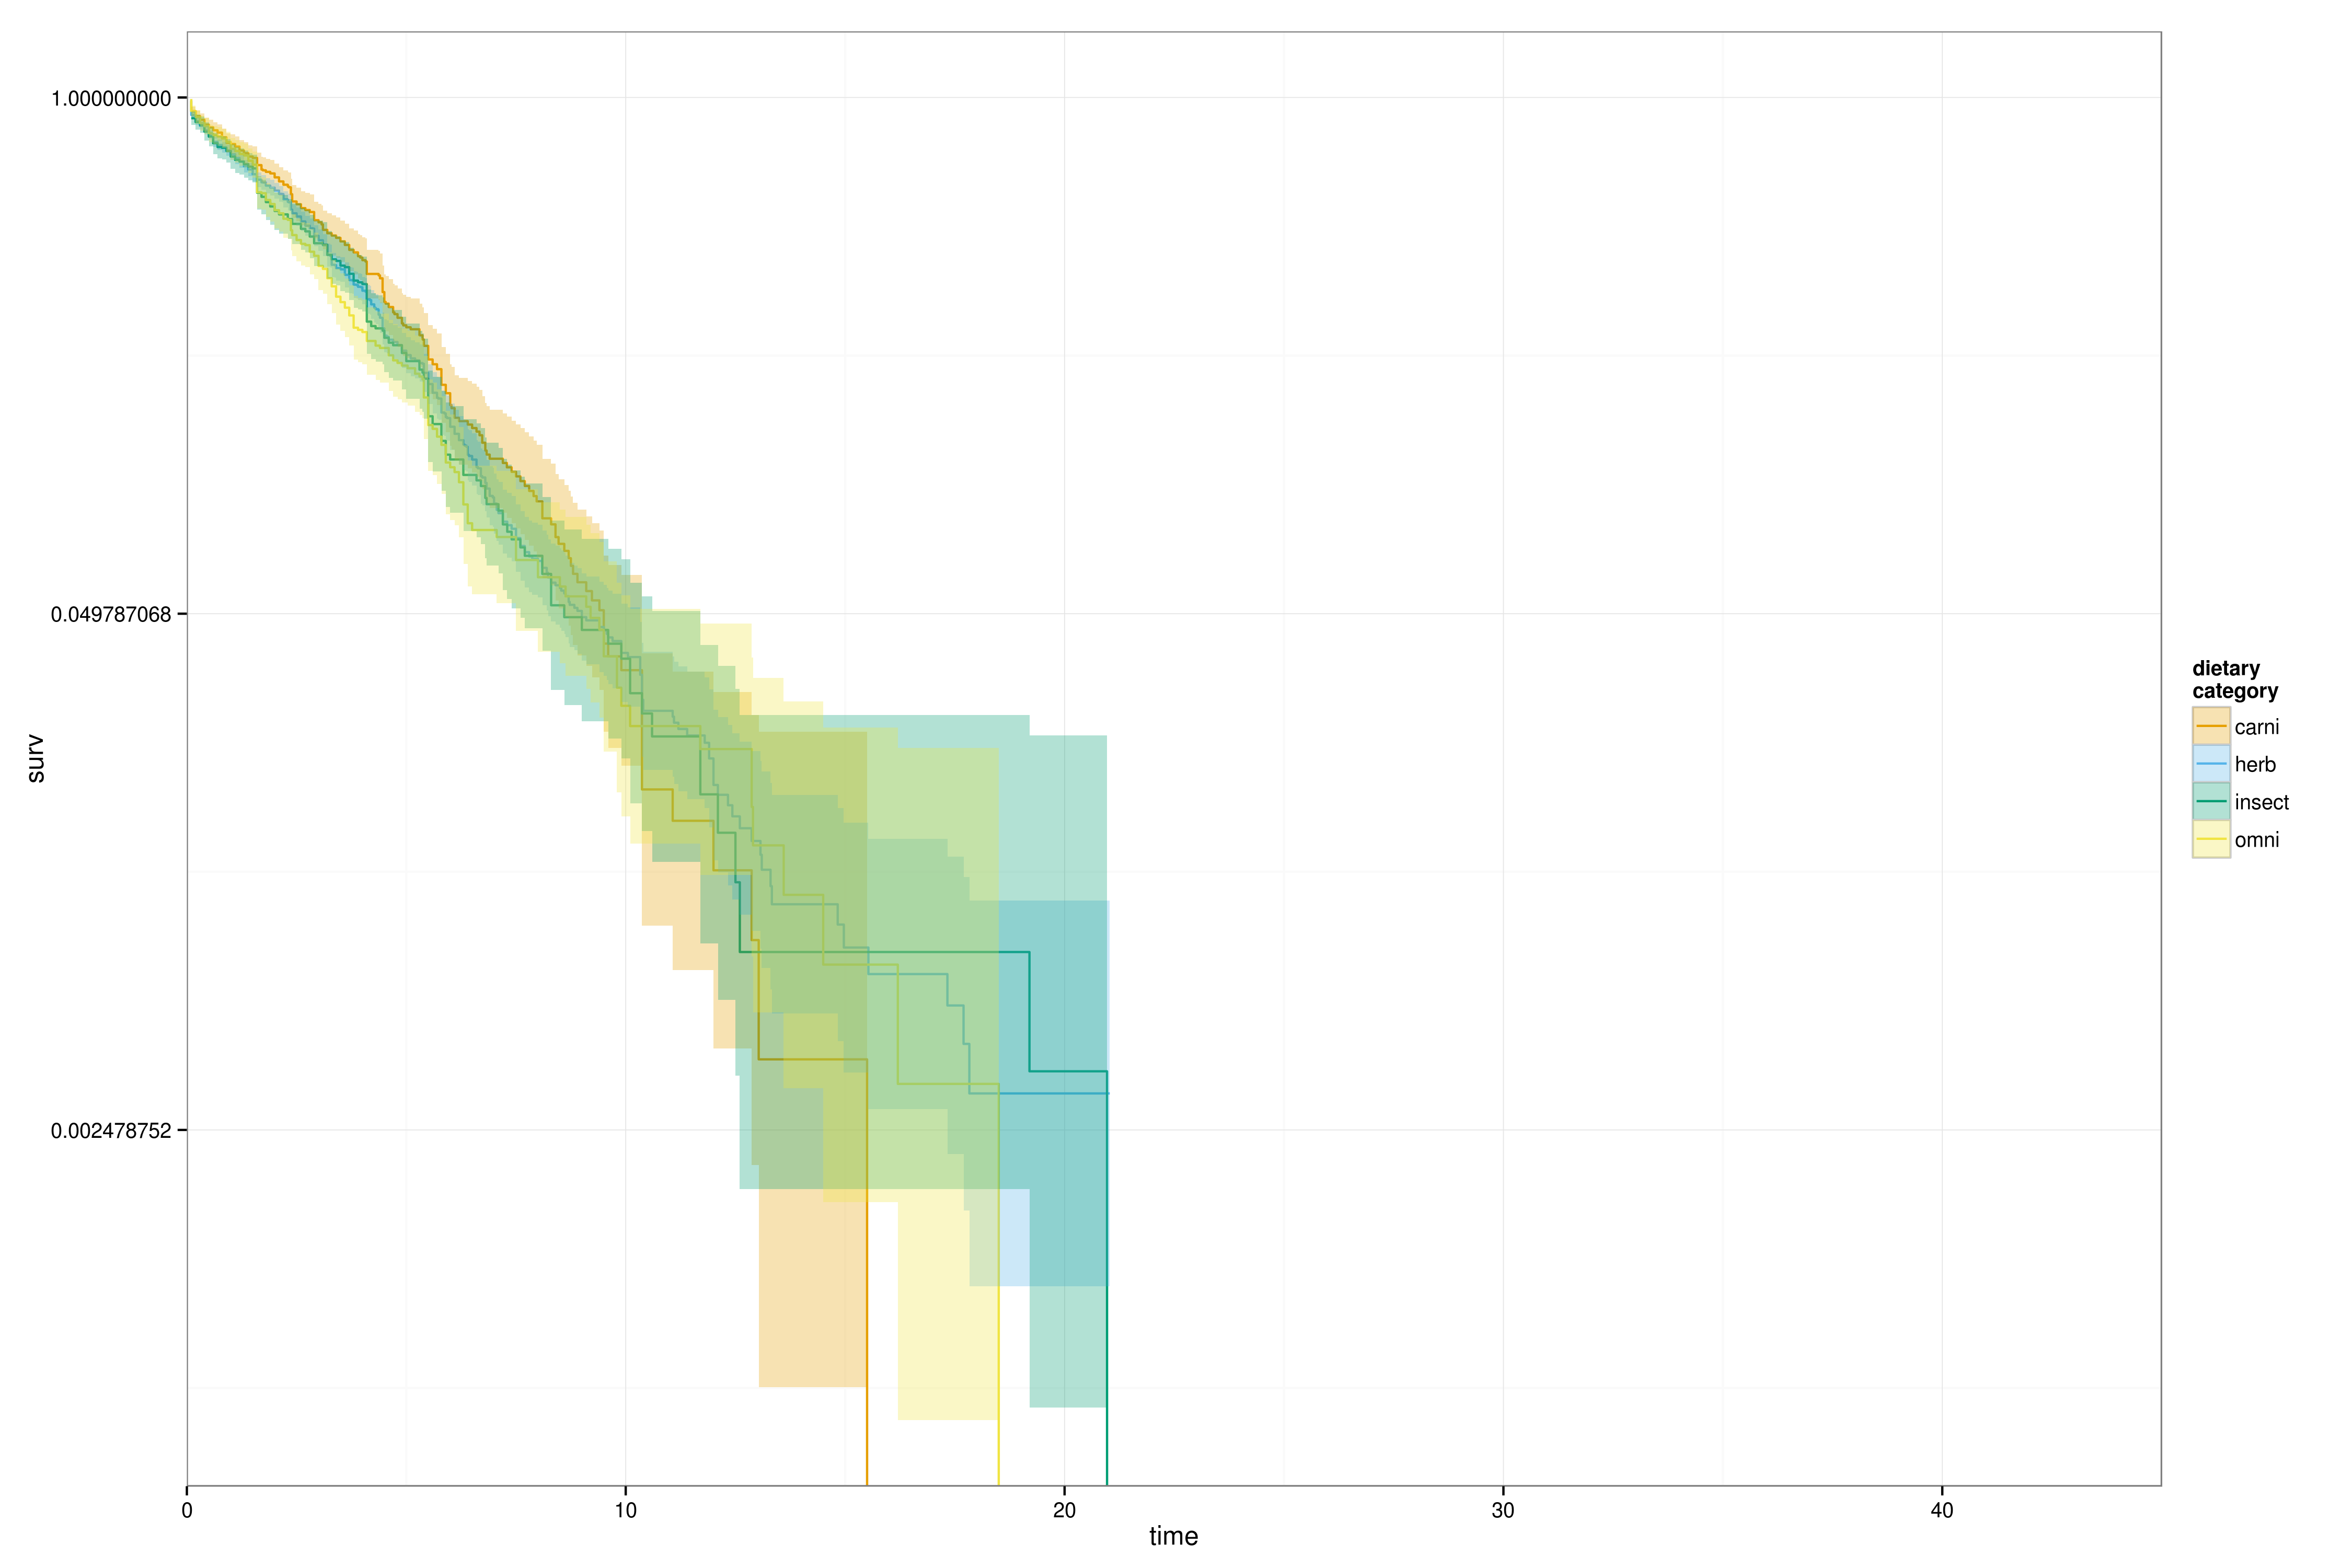
\includegraphics[width = \textwidth, keepaspectratio = true]{figure/km_nad}
      \label{subfig:km_nad}
    \end{subfigure}
    \begin{subfigure}[b]{0.4\textwidth}
      \caption{}
      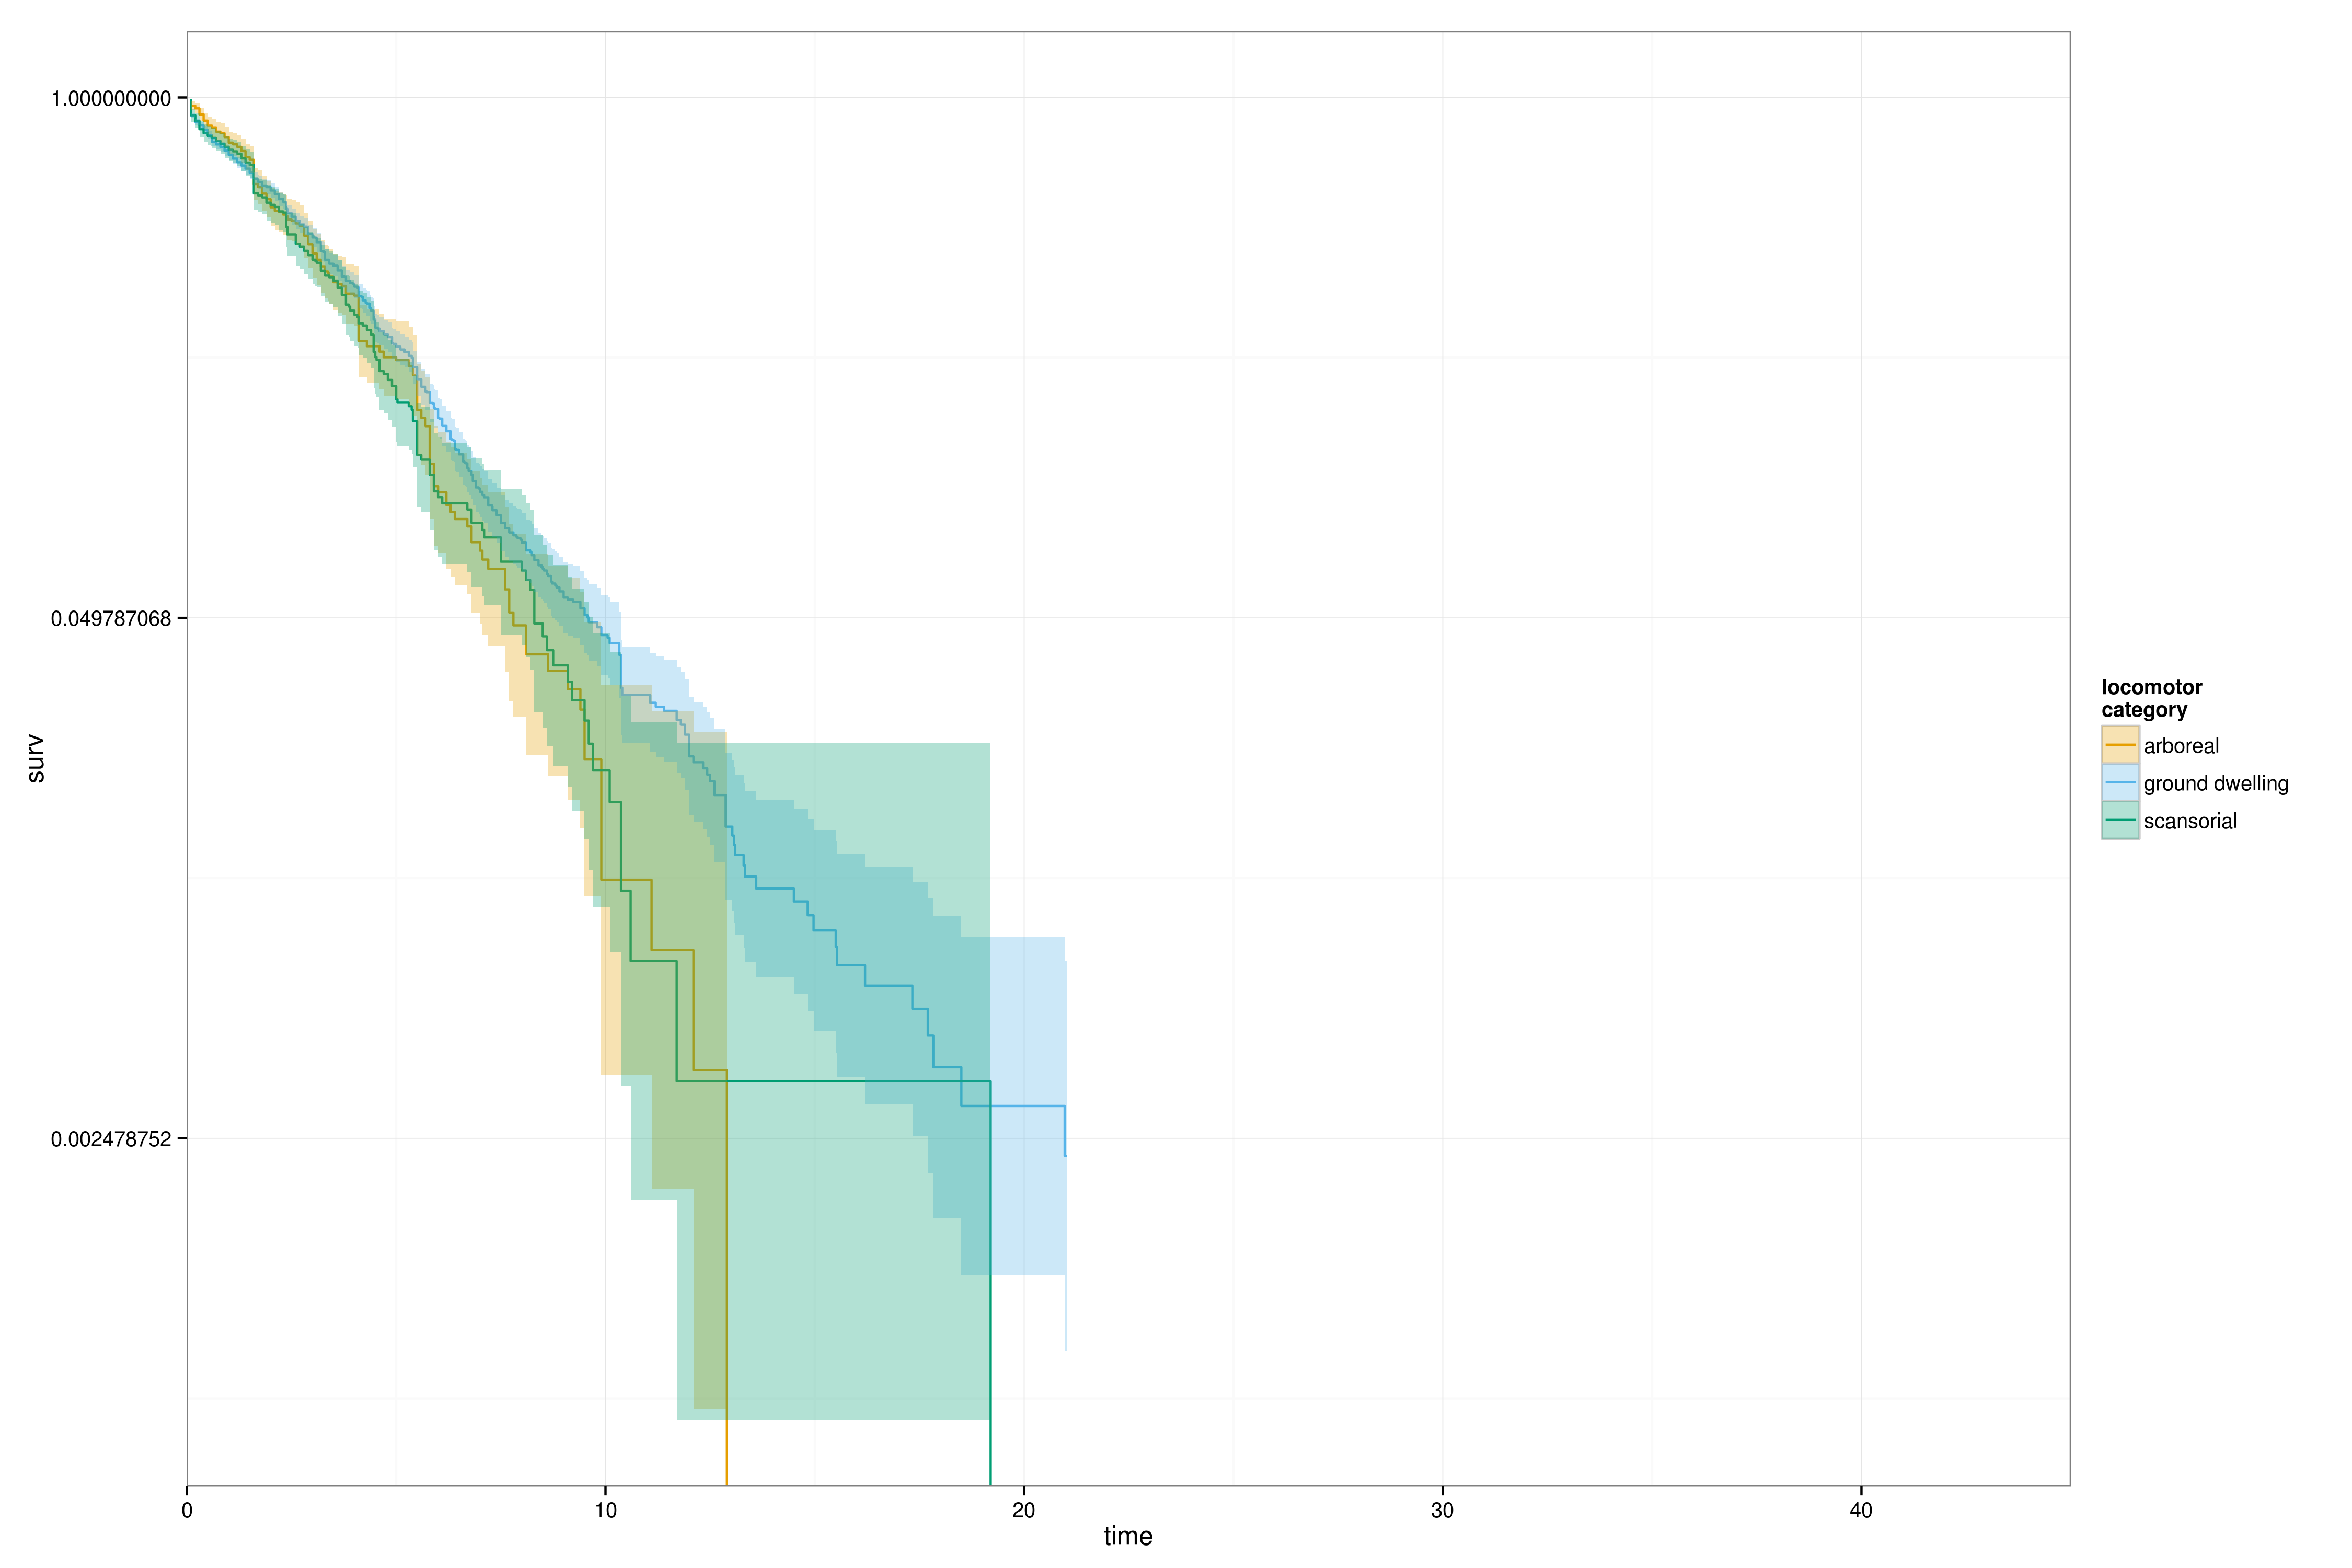
\includegraphics[width = \textwidth, keepaspectratio = true]{figure/km_nal}
      \label{subfig:km_nal}
    \end{subfigure}

    \begin{subfigure}[b]{0.4\textwidth}
      \caption{}
      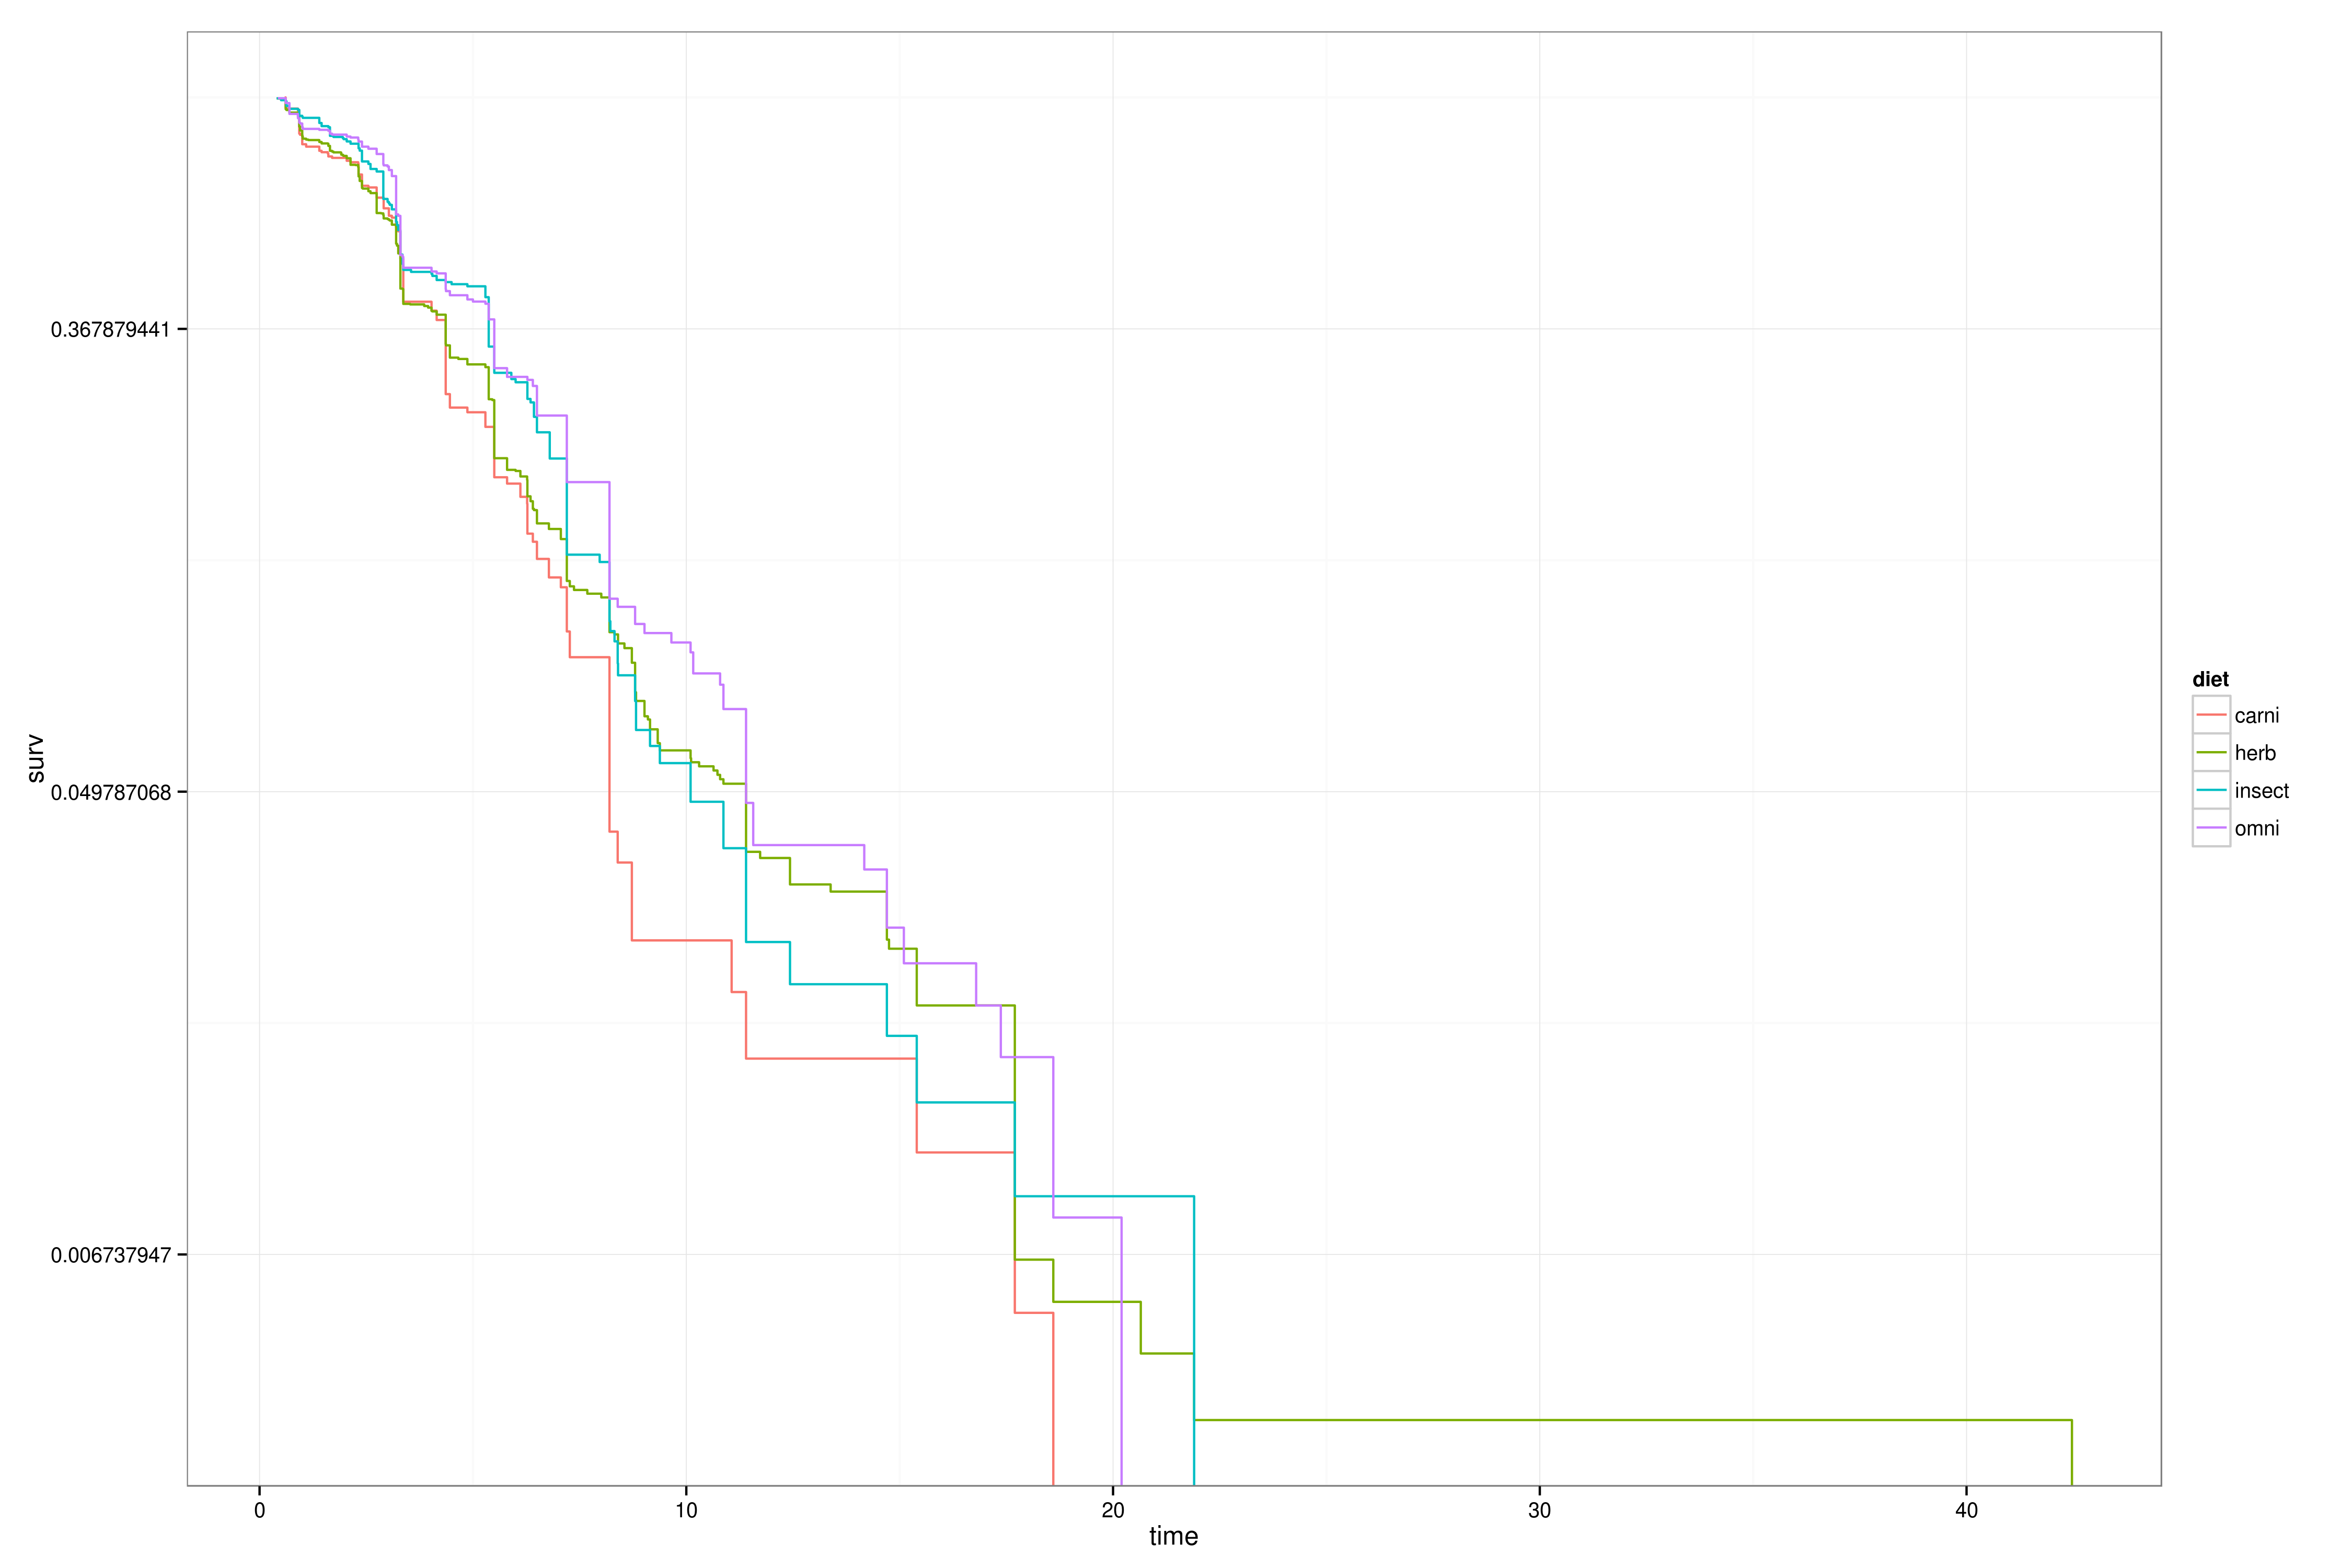
\includegraphics[width = \textwidth, keepaspectratio = true]{figure/km_erd}
      \label{subfig:km_erd}
    \end{subfigure}
    \begin{subfigure}[b]{0.4\textwidth}
      \caption{}
      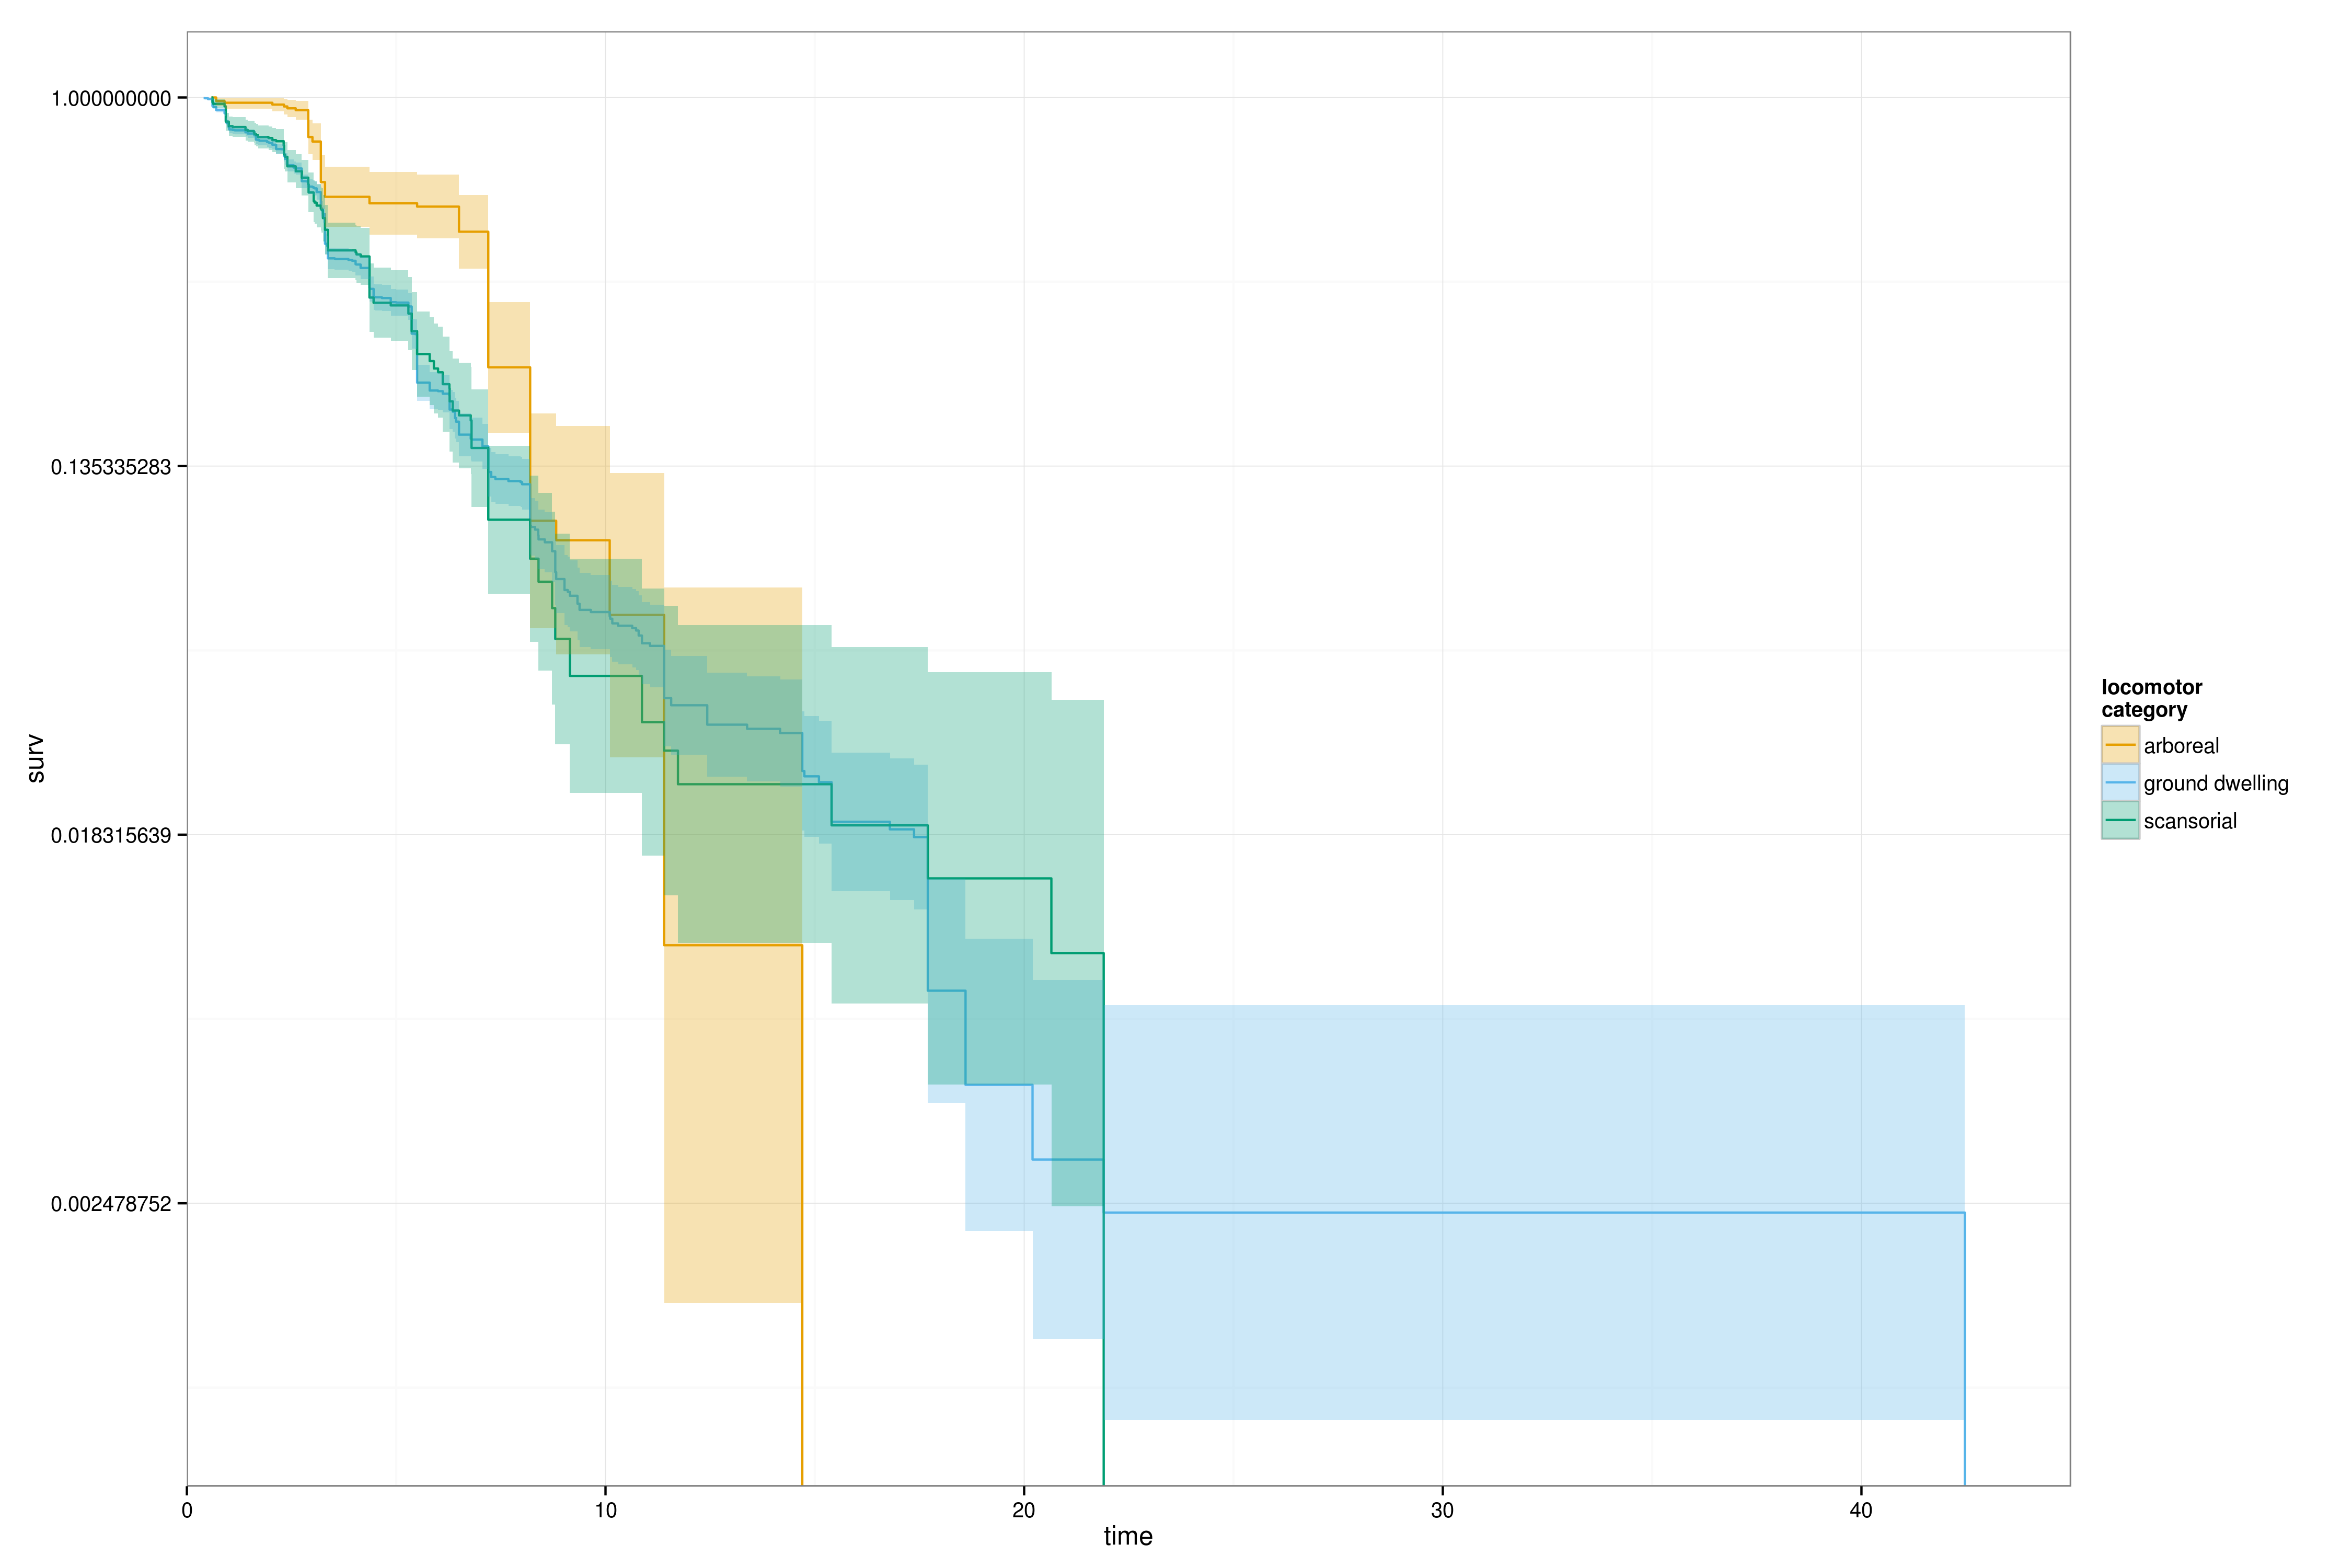
\includegraphics[width = \textwidth, keepaspectratio = true]{figure/km_erl}
      \label{subfig:km_erl}
    \end{subfigure}
  \end{center}
  \caption{Nonparametric Kaplan-Meier species-level survival curves for North American and European mammals based on dietary category (\subref{subfig:km_nad} and \subref{subfig:km_erd} respectively, and locomotor category (\subref{subfig:km_nal} and \subref{subfig:km_erl} respectively). K-M curves are illustrated with 95\% confidence intervals. The vertical axes are on a natural log scale.}
  \label{fig:mam_surv_curv}
\end{figure}

These results are extremely preliminary and based solely on qualitative patterns present in the nonparametric K-M survival curves and without reference to estimated median survival times. Additionally, possible differences in survival based on body-size were not estimated. Also, no comparison has been made with the different climatic histories of both Continents. By including all three time-independent covariates in a parametric modelling of survival framework it should be possible to better understand the underlying process behind survival. The inclusion of a third continent, South America, will also greatly improve the overall understanding of how extinction in mammals proceeds and how this may differ across environments.


\subsection{Community connectedness: global, regional, local} \label{sec:mamcom}

\subsubsection{Questions} \label{sec:mamcomques}
How does the ratio between endemic and cosmopolitan taxa at a locality change over time? Is this pattern different between ecological categories? Does this pattern reflect global, regional, and/or local processes? 

\subsubsection{Background and Predictions} \label{sec:mamcomback}
During the Cenozoic there was a global shift from a ``hot house'' environment to an ``ice house'' environment \citep{Zachos2008,Zachos2001}. This transition was accompanied by major shifts in global climatic envelopes and the reorganization of mammalian communities \citep{Janis1993a,Fortelius2002,Blois2009,Alroy2000g,Figueirido2012}. For mammalian community connectedness there are two possible scenarios. First, while the environment was shifting, lineages may have adapted in place and overall trophic structure and community connectedness would have remained relatively constant through time, as observed during the Neogene of Europe \citep{Jernvall2004}. Alternatively, species may have shifted ranges and changed the average set of taxa present at a locality which would be associated with non-stationary trophic structure and community connectedness.

Based on prior work, it is expected that the patterns of biogeographic community connectedness for herbivorous taxa in a region would be most similar to that for all regional taxa and potentially ``drive'' the regional pattern, partially because on average this category represents the majority or plurality of taxa \citep{Jernvall2002}. In contrast, community connectedness for carnivorous taxa is expected to remain constant over time or be correlated with herbivore patterns. Finally, omnivorous taxa are not expected to be correlated with the patterns of either herbivorous or carnivorous taxa and have either a relatively constant or random pattern of connectedness over time.  These predictions are based on the differences in resilience and relationship to primary productivity, with herbivores being more resilient than carnivores and omnivores being random in their resilience \citep{Jernvall2004}. Resilience is defined here as the ability for a taxon to increase in occupancy following a decline \citep{Jernvall2004}.

The Cenozoic global shift from closed, forested habitat in the Paleogene to open, savanna-like habitat during the Neogene would have greatly affected the possible distributions of both arboreal and ground dwelling taxa. Additionally, the timing of this environmental shift was different between continents \citep{Stromberg2005,Stromberg2013}, so patterns of community connectedness may not be globally uniform and instead reflect regional differences. Generally this transitions would cause forested environments to become increasingly patchier in distribution while transitioning from the Paleogene to the Neogene. The global prediction then is that there would have been a relative increase in \(E\) (Eq. \ref{eq:e}) and code length accompanied by a decrease in \(BC\) (Eq. \ref{eq:bc}) and \(Occ\) (Eq. \ref{eq:occ}) in arboreal taxa over time. The opposite is expected for terrestrial taxa. 

At a regional scale, North American community connectedness is expected to follow the global predictions described above because the vast amount of prior synthesis has focused on North America \citep{Alroy2000g,Alroy1996a,Alroy1998,Barnosky2001a,Simpson1944,Simpson1953,Badgley2013,Blois2009,Figueirido2012,Gunnell1995,Hadly2001}. However, the effect of global climate change on North American diversity remains unresolved and controversial \citep{Alroy2000g,Blois2009,Figueirido2012,Barnosky2001a}, thus it is necessary to determine empirically when global versus regional versus local scale processes may have dominated and how that may have changed over time.

The European mammalian fossil record is also well studied, though research has primarily focused on the Neogene \citep{Jernvall2002,Jernvall2004,Liow2008,Raia2006,Raia2005,Raia2011c}. An important aspect about the European record is that during the Neogene there was little shift in relative dietary category abundance \citep{Jernvall2004} and that the patterns within herbivores (browse--graze transition) were mostly driven by abundant, cosmopolitan taxa \citep{Jernvall2002}. It is predicted then that herbivores will demonstrate the same patterns of community connectedness as Europe as a whole, while omnivores and carnivores will be different from that of herbivores and may demonstrate random or constant patterns of community connectedness through time. 

Patterns of community connectedness for South American mammalian fauna are comparatively less synthesized than those of North American and Europe. Instead, cross--continental dynamics between North and South America during the Neogene are much more studied \citep{Marshall1982}. The South American mammalian faunal record reflects two distinct biotic provinces between the North and the South \citep{Macfadden1997,Macfadden2006,Flynn1998a,Patterson1968}. Because of this, it is expected that South America will have a different pattern of community connectedness than either North America or Europe. Also, there is an expected dramatic increase occupancy in land-dwelling herbivores relative to arboreal and scansorial taxa related to the aridification of high--latitude South America. Additionally, because of this strong biome distinction, it is predicted that provinciality will be high but remain constant over time. % improve this a lot following Dave Polly's comments

\subsubsection{Proposed research} \label{sec:mamcommeth}
In order to estimate changes in community connectedness during the Cenozoic I will be using the network-based approach described above (Section \ref{sec:bionet}). Biogeographic networks will be constructed for each region (North America, Europe, South American) between species and localities defined as 2x2 latitude--longitude grid cells from an equal-area map projection. Networks will be made for every 2 My span of the Cenozoic. This bin width was chosen to in order to maximize the chance that two localities are present at the same time. Networks will also be constructed for subsets of taxa defined by dietary and locomotor categories order to compare patterns both within and between categories, as well as to the combined regional and global patterns. Because previous studies of mammalian occurrence patterns have restricted analysis to large bodied and well studied groups such as Primates and Artiodactyls in order to account for potential sampling and taxonomic biases, analysis will be done using all available taxa and with a restricted sample of just major groups in order to observe any differences in patterns of community connectedness.  The data necessary to complete this study is the same as for the above analysis of mammalian survival (Section \ref{sec:mamsurv}).

The degree of phylogenetic similarity between taxa at a locality may play an important role in community structuring \citep{Webb2002}. For example, closely related taxa may be repulsed ``repulsed'' due to competitive exclusion or ``clumped'' because of environmental filtering. While it is infeasible to create an explicit phylogenetic hypothesis for all taxa sampled on all continents, almost all taxa have some hierarchical taxonomic information. Using taxonomy as the structure of an information phylogeny, it should be possible to estimate the distribution of phylogenetic similarity across localities.

For each locality, an informal phylogeny will be constructed based solely on available taxonomic information such as order, family, and genus assignments with each of these levels being a completely unresolved polytomy. Using this informal phylogeny, a number of measures of phylogenetic similarity can be estimated. For example the relative mean pairwise distance between all taxa at a locality \citep{Webb2002} or the related phylogenetic species variability of a single locality \citep{Helmus2007a}. These values calculated for all localities can then be used as a partial correlates or covariates when modeling changes in community connectedness.

As with the Permian brachiopods (Section \ref{sec:braccom}), patterns of community connectedness will be compared both within and between ecological categories. Additionally, the correspondence of changes in environmental conditions and community connectedness will also be analysed. The approach and methodology to accomplish these analyses is currently under development. Additionally, the possibility of integrating locality--locality distance or some other measure of topology will be explored, especially how this relates to code length and provinciality in general.


\subsubsection{Preliminary results} \label{mamcomres}
Preliminary analysis was done using only the occurrence information of both North American and European fossil mammals available in the PBDB. Both regions have qualitatively different patterns of community connectedness, primarily during the Paleogene (Fig. \ref{fig:mam_con}). Almost all four of the summary statistics are extremely volatile over the Cenozoic, especially for Europe. However, some interesting qualitative patterns are present. Importantly, the network summary statistics will be calculated only with reference to the localities at which arboreal taxa occur, and not all possible localities occurring at a specific time.

\begin{figure}[ht]
  \begin{center}
    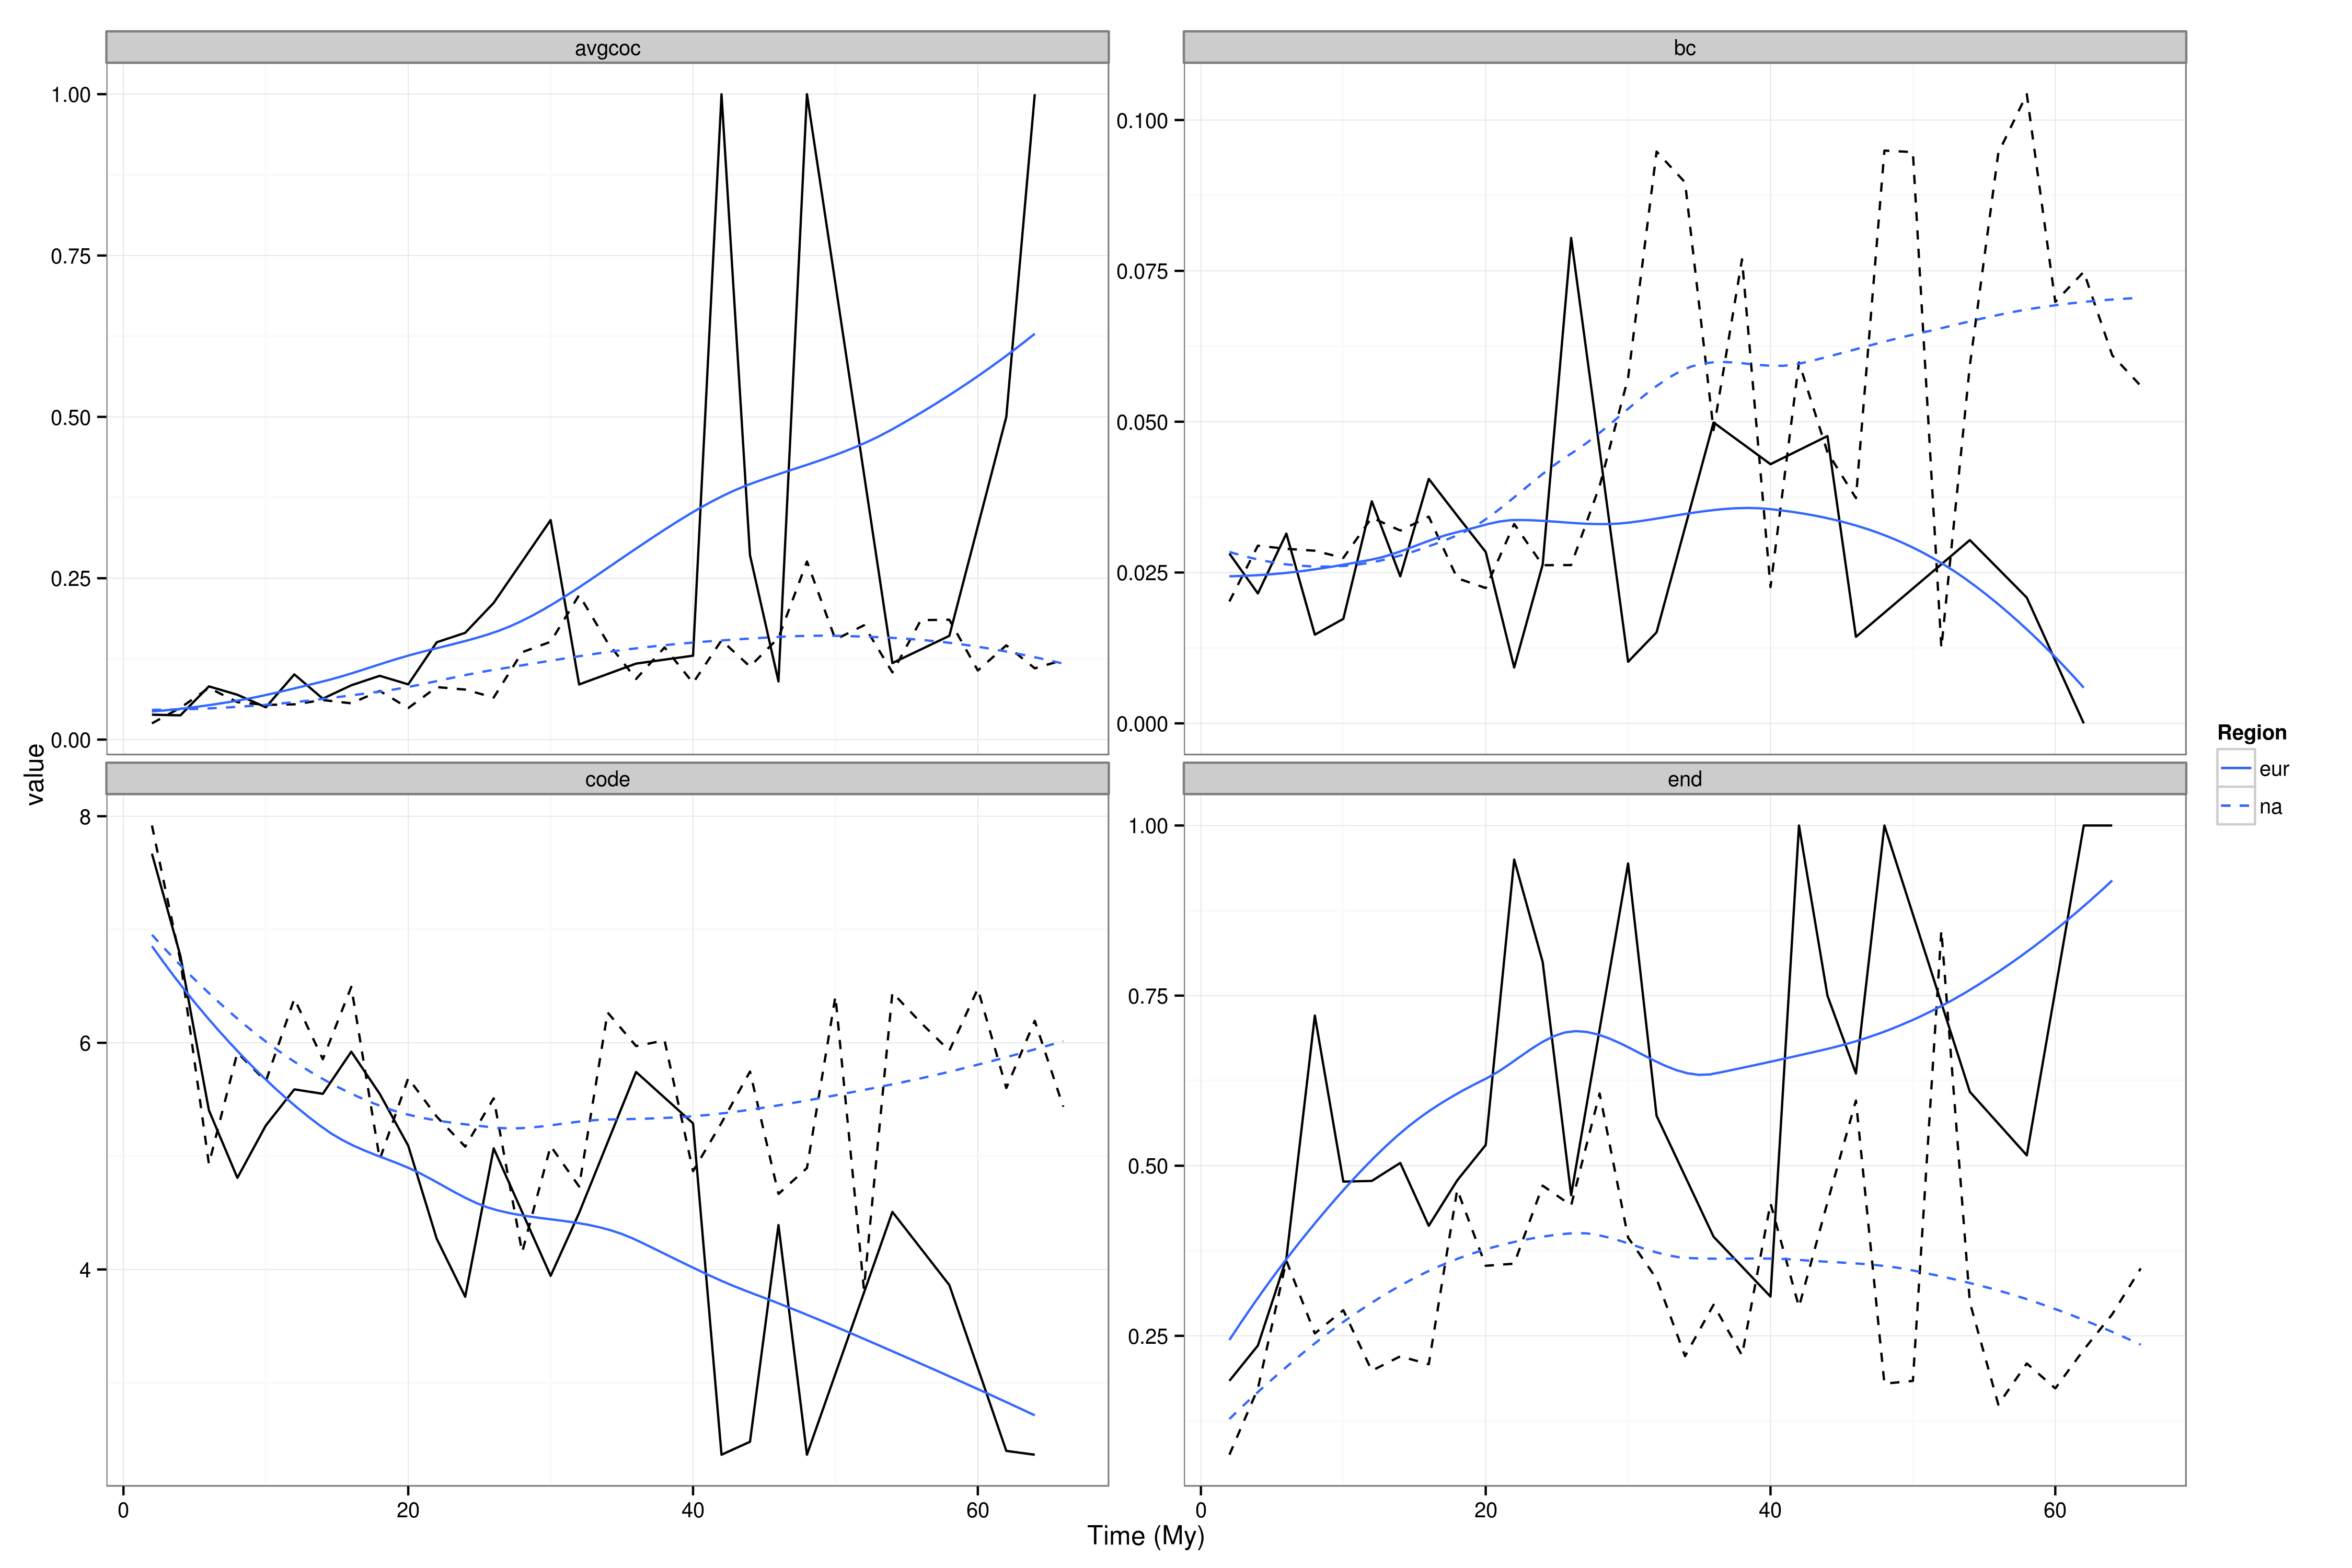
\includegraphics[height = 0.4\textheight, keepaspectratio = true]{figure/gen_bin}
  \end{center}
  \caption[North American and European community connectedness]{Biogeographic network summary statistics for mammalian communities in North America (dashed line) and Europe (solid line). The summary statistics are, clockwise from top left: biogeographic connectedness (BC), code length, average relative locality occupancy per taxon (Occ), and average relative number of endemic taxa per locality (E). Blue lines are generalized additive model smooths and are presented to illustrate the overall pattern for each region.} 
  \label{fig:mam_con}
\end{figure}

There is a qualitative decrease in \(Occ\) in Europe until approximately the start of the Neogene (approximately 23 My), indicating that the average taxon is becoming generally less cosmopolitan over time. In contrast, North American \(Occ\) is qualitatively stationary over the entire Cenozoic and almost always lower than that observed for Europe. This means that, on average, North American taxa are present in very few localities at any given point in time.

In Europe there is a qualitative rise in \(BC\) in the first few million years of the Cenozoic, but afterwards remains relatively stationary meaning that the average proportion of shared taxa remained qualitatively stationary. In comparison, North American \(BC\) remains stationary with a greater amount of shared taxa than Europe for the first half of the Cenozoic followed by a decrease and another plateau at the end of the Cenozoic.

In Europe, there is a over all qualitative decrease in \(E\) while in North America there is a qualitatively constant \(E\) over the Cenozoic with a slight decrease in the Neogene. As discussed above, \(E\) is a measure of relative uniqueness of a locality on average. Qualitatively, North America retained approximately the same amount of site uniqueness through out the Cenozoic. While the pattern of the European record shows a qualitatively nonmonotonic decrease in locality uniqueness.

The code length of European biogeographic networks increases qualitatively over the entire Cenozoic, while code length of North American networks remains relatively constant until the Neogene when there is a qualitative increase. Initial interpretation of these results indicates that North America maintains a relatively stationary degree of provinciality while Europe has a qualitatively decreasing degree of provinciality. 

\begin{figure}[ht]
  \begin{center}
    \begin{subfigure}[b]{0.4\textwidth}
      \caption{}
      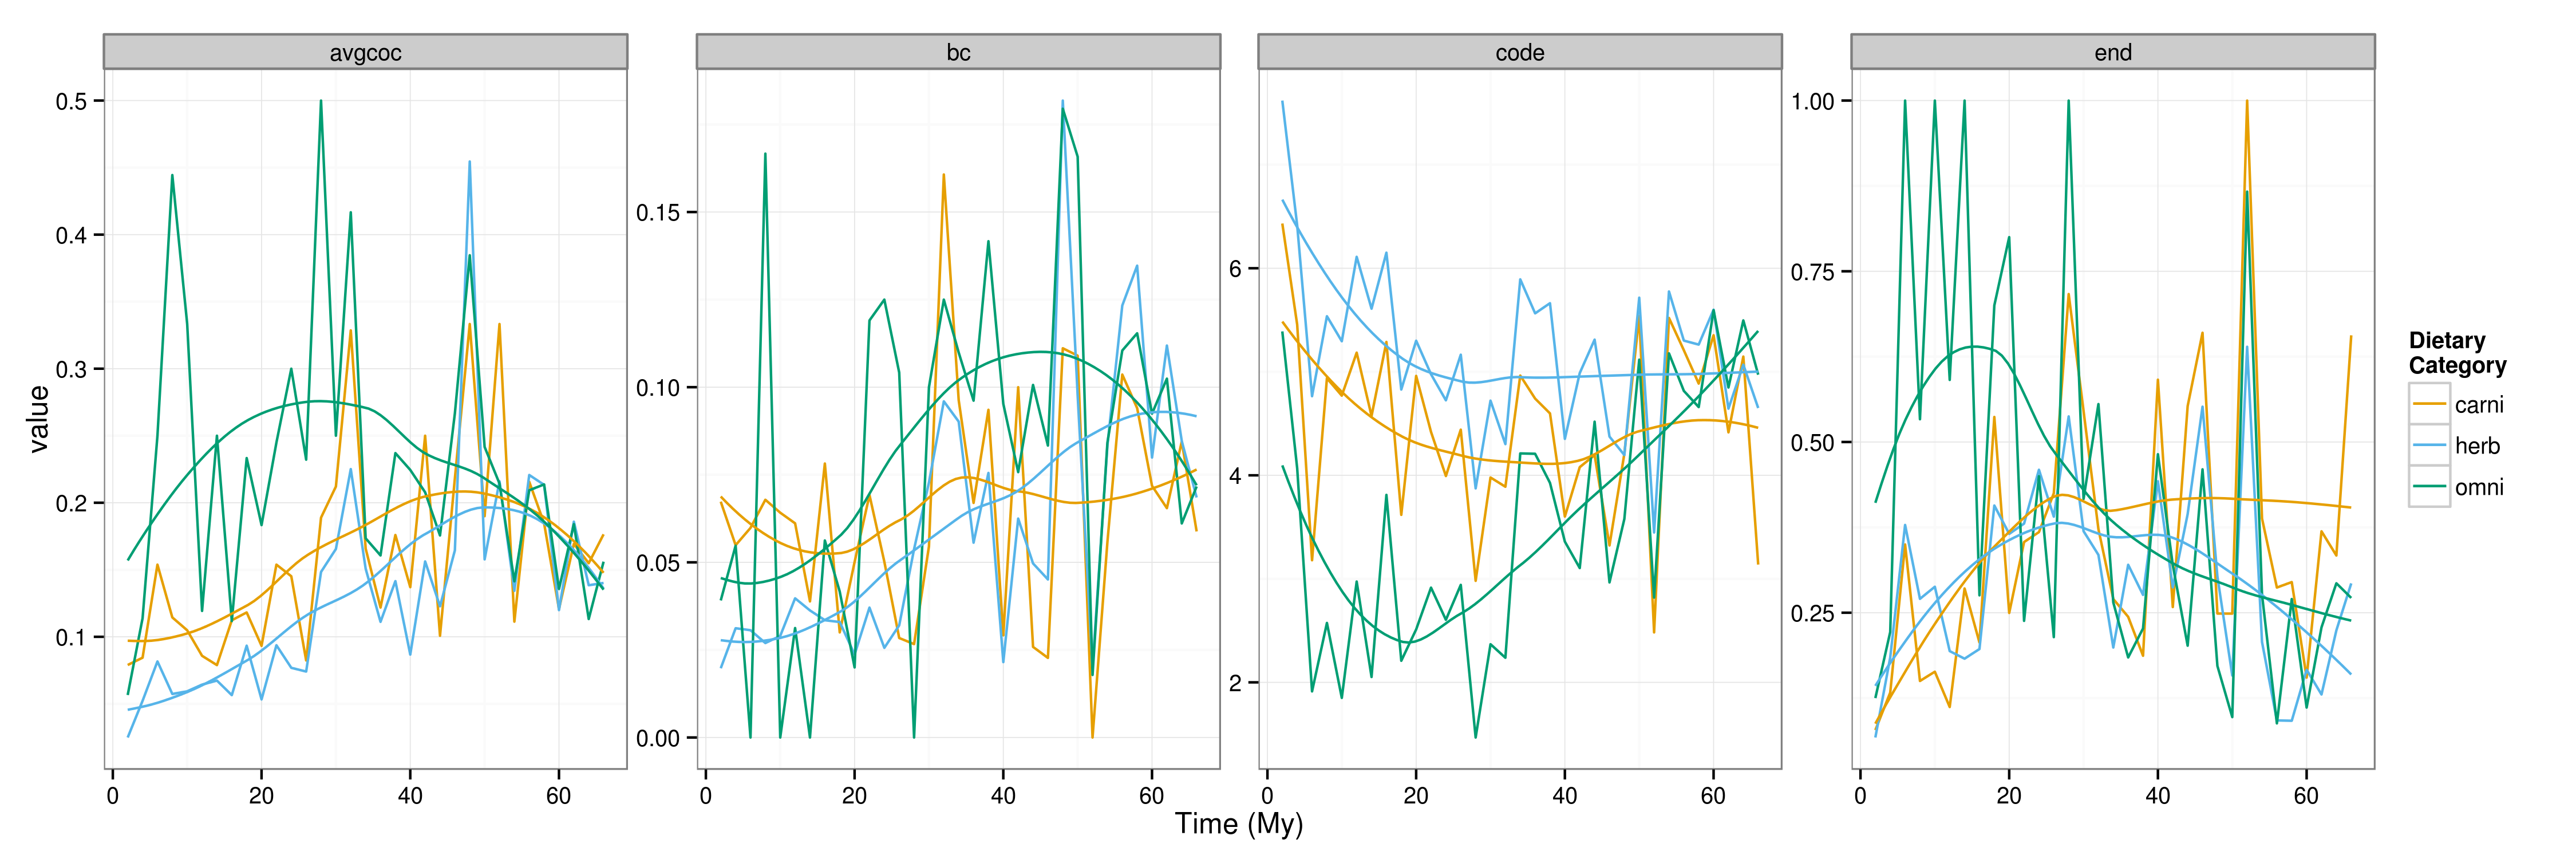
\includegraphics[width = \textwidth, keepaspectratio = true]{figure/na_dt}
      \label{subfig:diet_con_na}
    \end{subfigure}
    \begin{subfigure}[b]{0.4\textwidth}
      \caption{}
      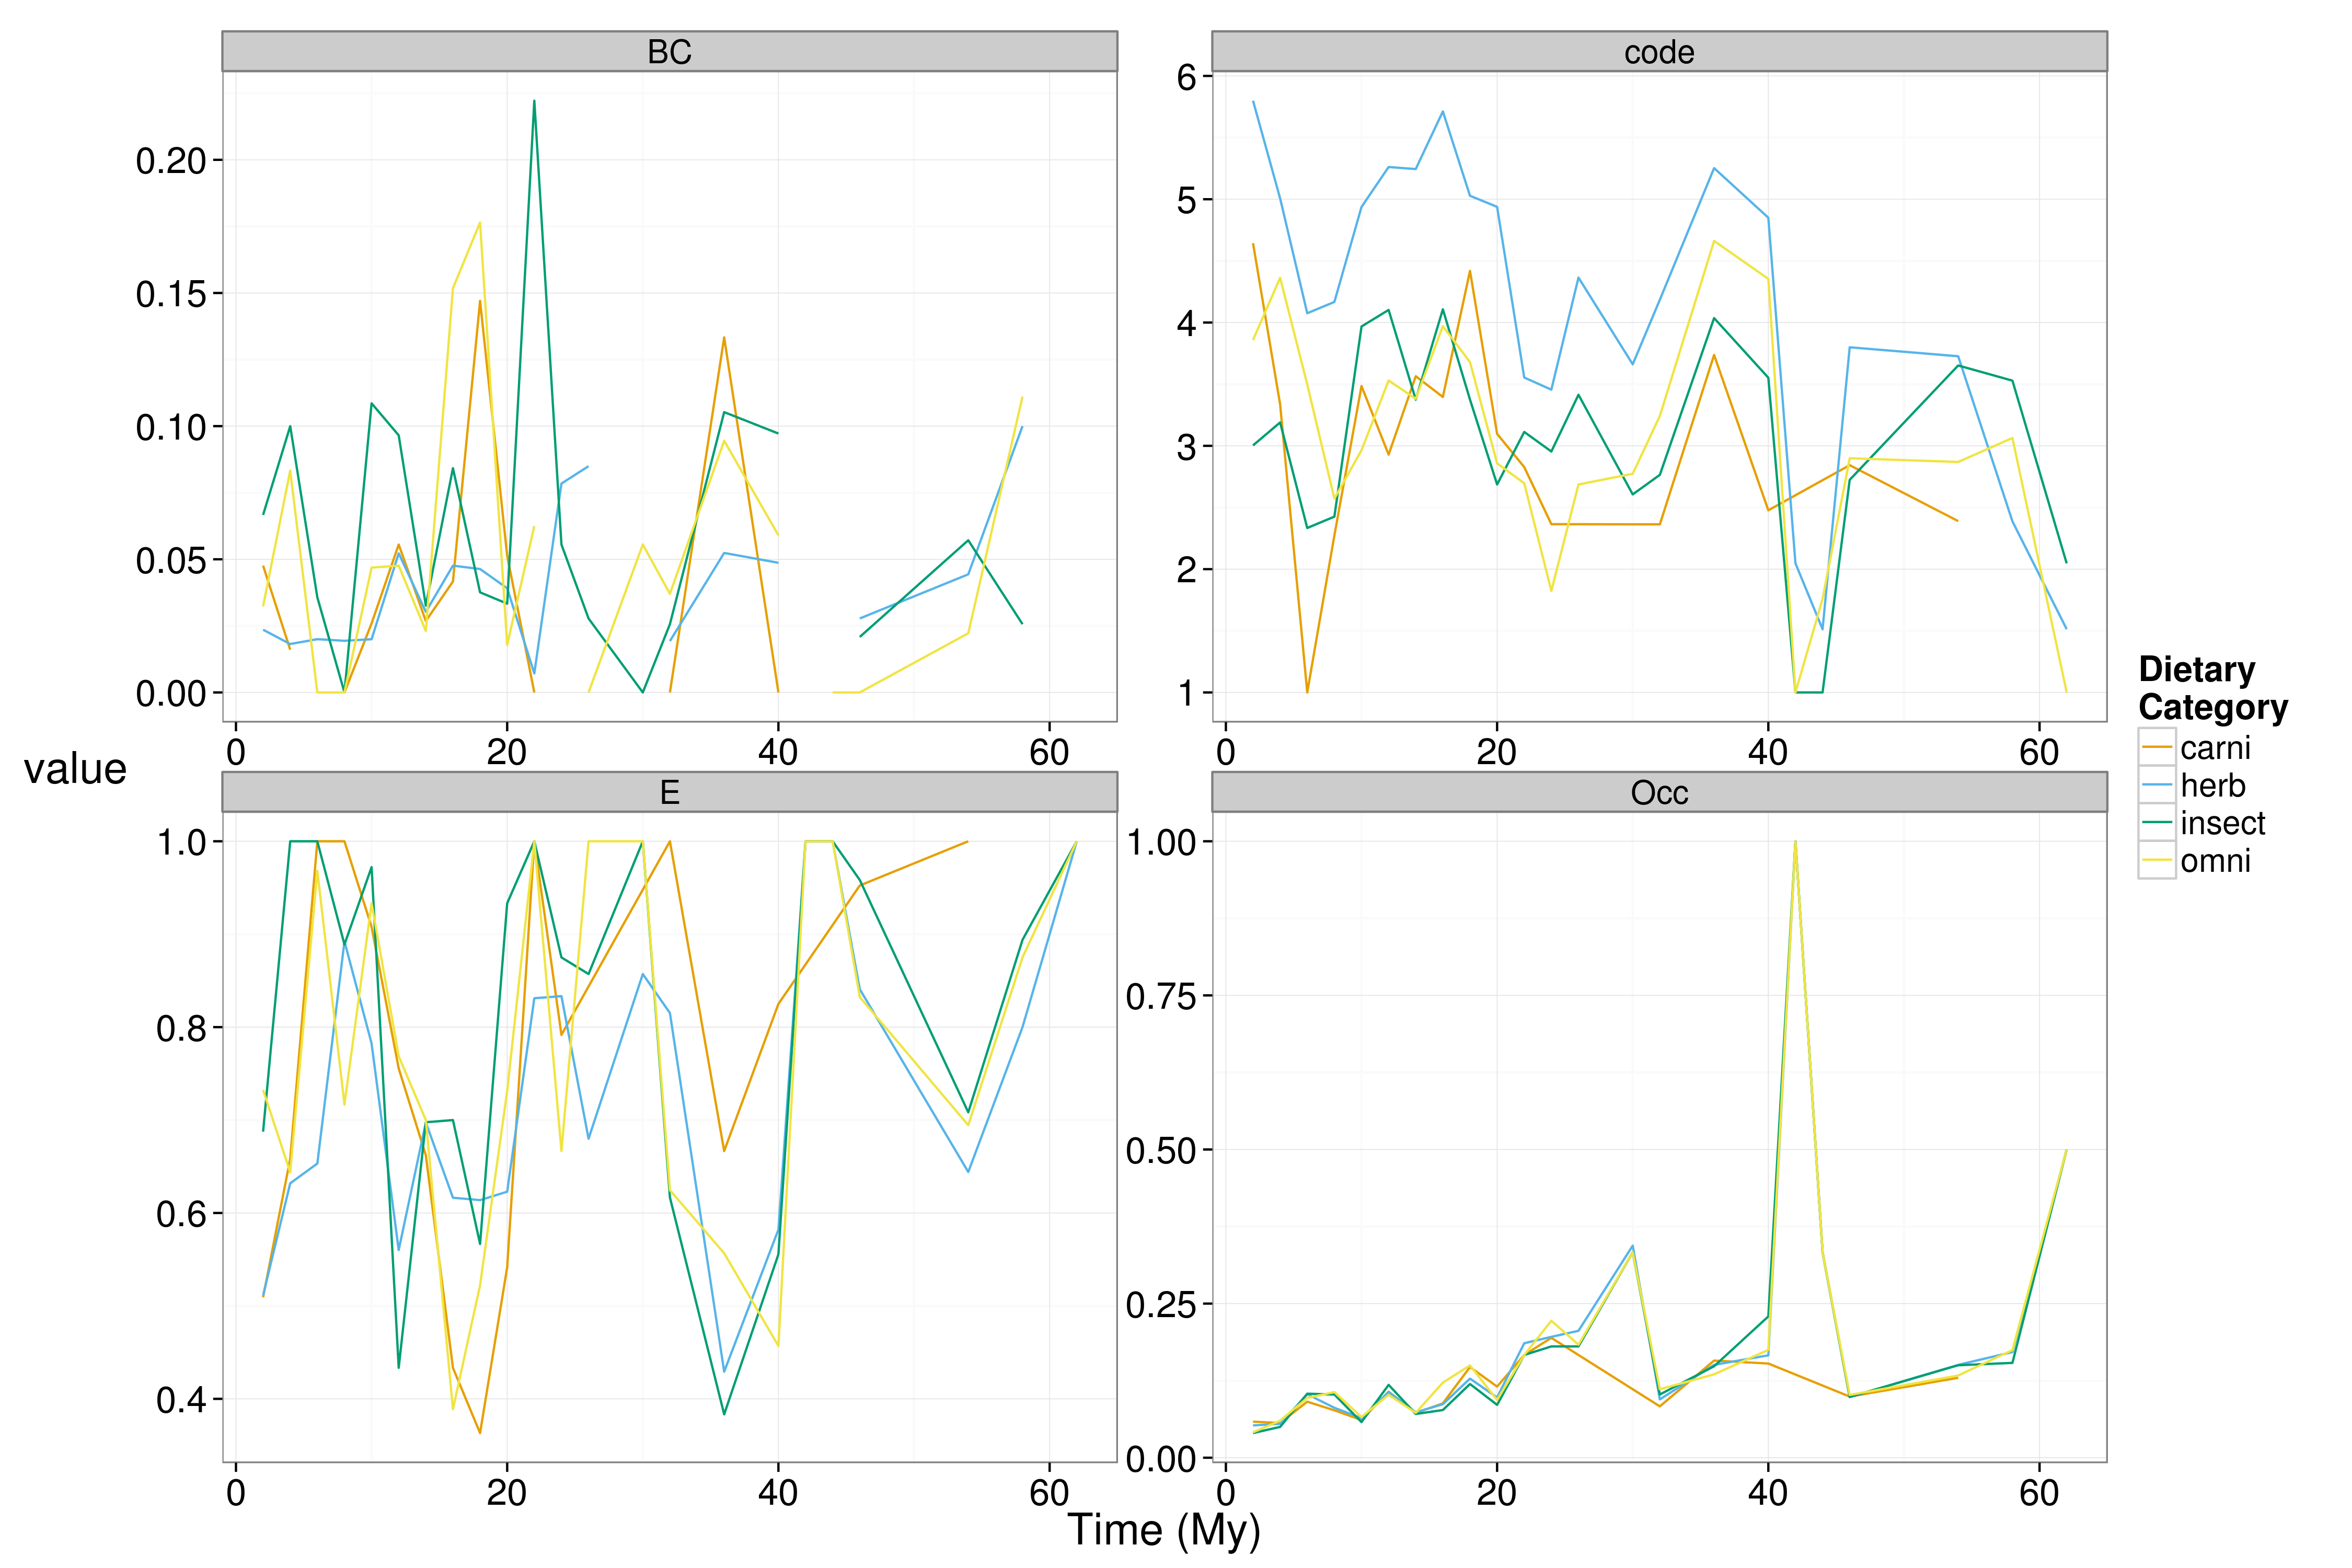
\includegraphics[width = \textwidth, keepaspectratio = true]{figure/er_dt}
      \label{subfig:diet_con_er}
    \end{subfigure}
  \end{center}
  \caption[Dietary category based community connectedness]{Time series of summary statistics for biogeographic networks determined by dietary category for North America (\subref{subfig:diet_con_na}) and Europe (\subref{subfig:diet_con_er}). The summary statistics are, clockwise from top left: biogeographic connectedness (BC), code length, average relative locality occupancy per taxon (Occ), and average relative number of endemic taxa per locality (E).} 
  \label{fig:diet_con}
\end{figure}

When taxa are separated by dietary categories, the amount of noise associated with each statistic increases greatly (Fig. \ref{fig:diet_con}). In North America, \(BC\), while variable, appears to qualitatively demonstrate no net change. Carnivores and herbivores to qualitatively become less volatile during the Neogene compared to the Paleogene (Fig. \ref{subfig:diet_con_na}). \(BC\) for Europe is also very volatile, though impossible to measure for dietary categories individually for much of the Paleogene (Fig. \ref{subfig:diet_con_er}).

Code length for North American qualitatively shows a stationary pattern with an up-tick in the Recent and a major drop at approximately 50-55 My (Fig. \ref{subfig:diet_con_na}). Additionally, herbivore and carnivore patterns appear qualitatively similar. In comparison, the European record for code length shows a qualitatively slight increase over the entire Cenozoic (Fig. \ref{subfig:diet_con_er}). Also, the patterns of herbivore and carnivores appear qualitatively less similar than for North America. For both Europe and North America, herbivores have the over all highest code length. In North America, carnivores arguably have the second highest code length. In all other cases, the ranks are qualitatively ambiguous.

\(E\) for North American appears to qualitatively have two categories (Fig. \ref{subfig:diet_con_na}). Herbivore and carnivore patterns are qualitatively stationary and low during the Neogene, while the omnivore and insectivore pattens are qualitatively more variable and higher during the Neogene. In comparison, all four categories of European mammals demonstrate a slight decrease during the Cenozoic (Fig. \ref{subfig:diet_con_er}).

For North America, \(Occ\) are qualitatively stationary throughout the Cenozoic with one spike in carnivore \(Occ\) at approximately 50-55 My (Fig. \ref{subfig:diet_con_na}). In contrast, European values are highly volatile throughout the Paleogene and then less volatile during the Neogene (Fig. \ref{subfig:diet_con_er}).

\begin{figure}[ht]
  \begin{center}
    \begin{subfigure}[b]{0.4\textwidth}
      \caption{}
      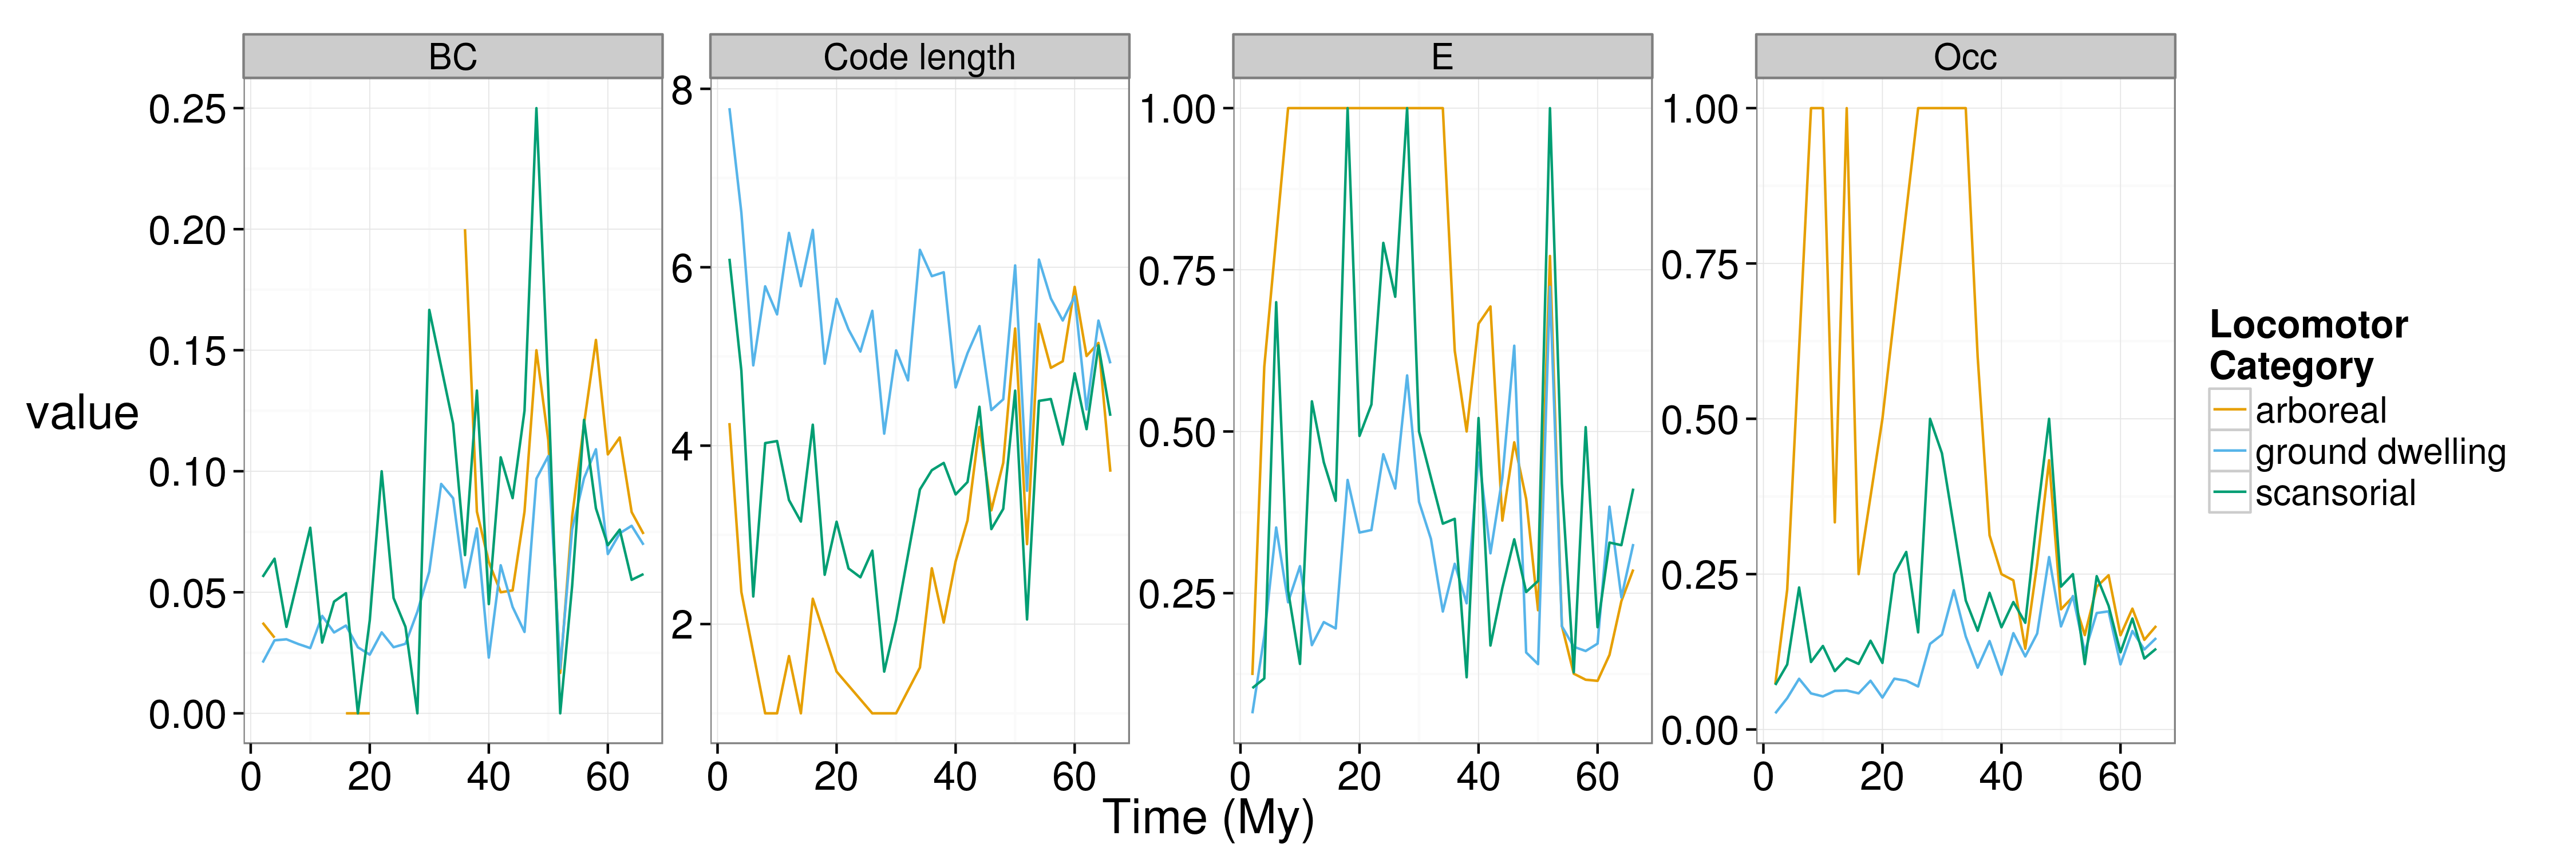
\includegraphics[width = \textwidth, keepaspectratio = true]{figure/na_lf}
      \label{subfig:loco_con_na}
    \end{subfigure}
    \begin{subfigure}[b]{0.4\textwidth}
      \caption{}
      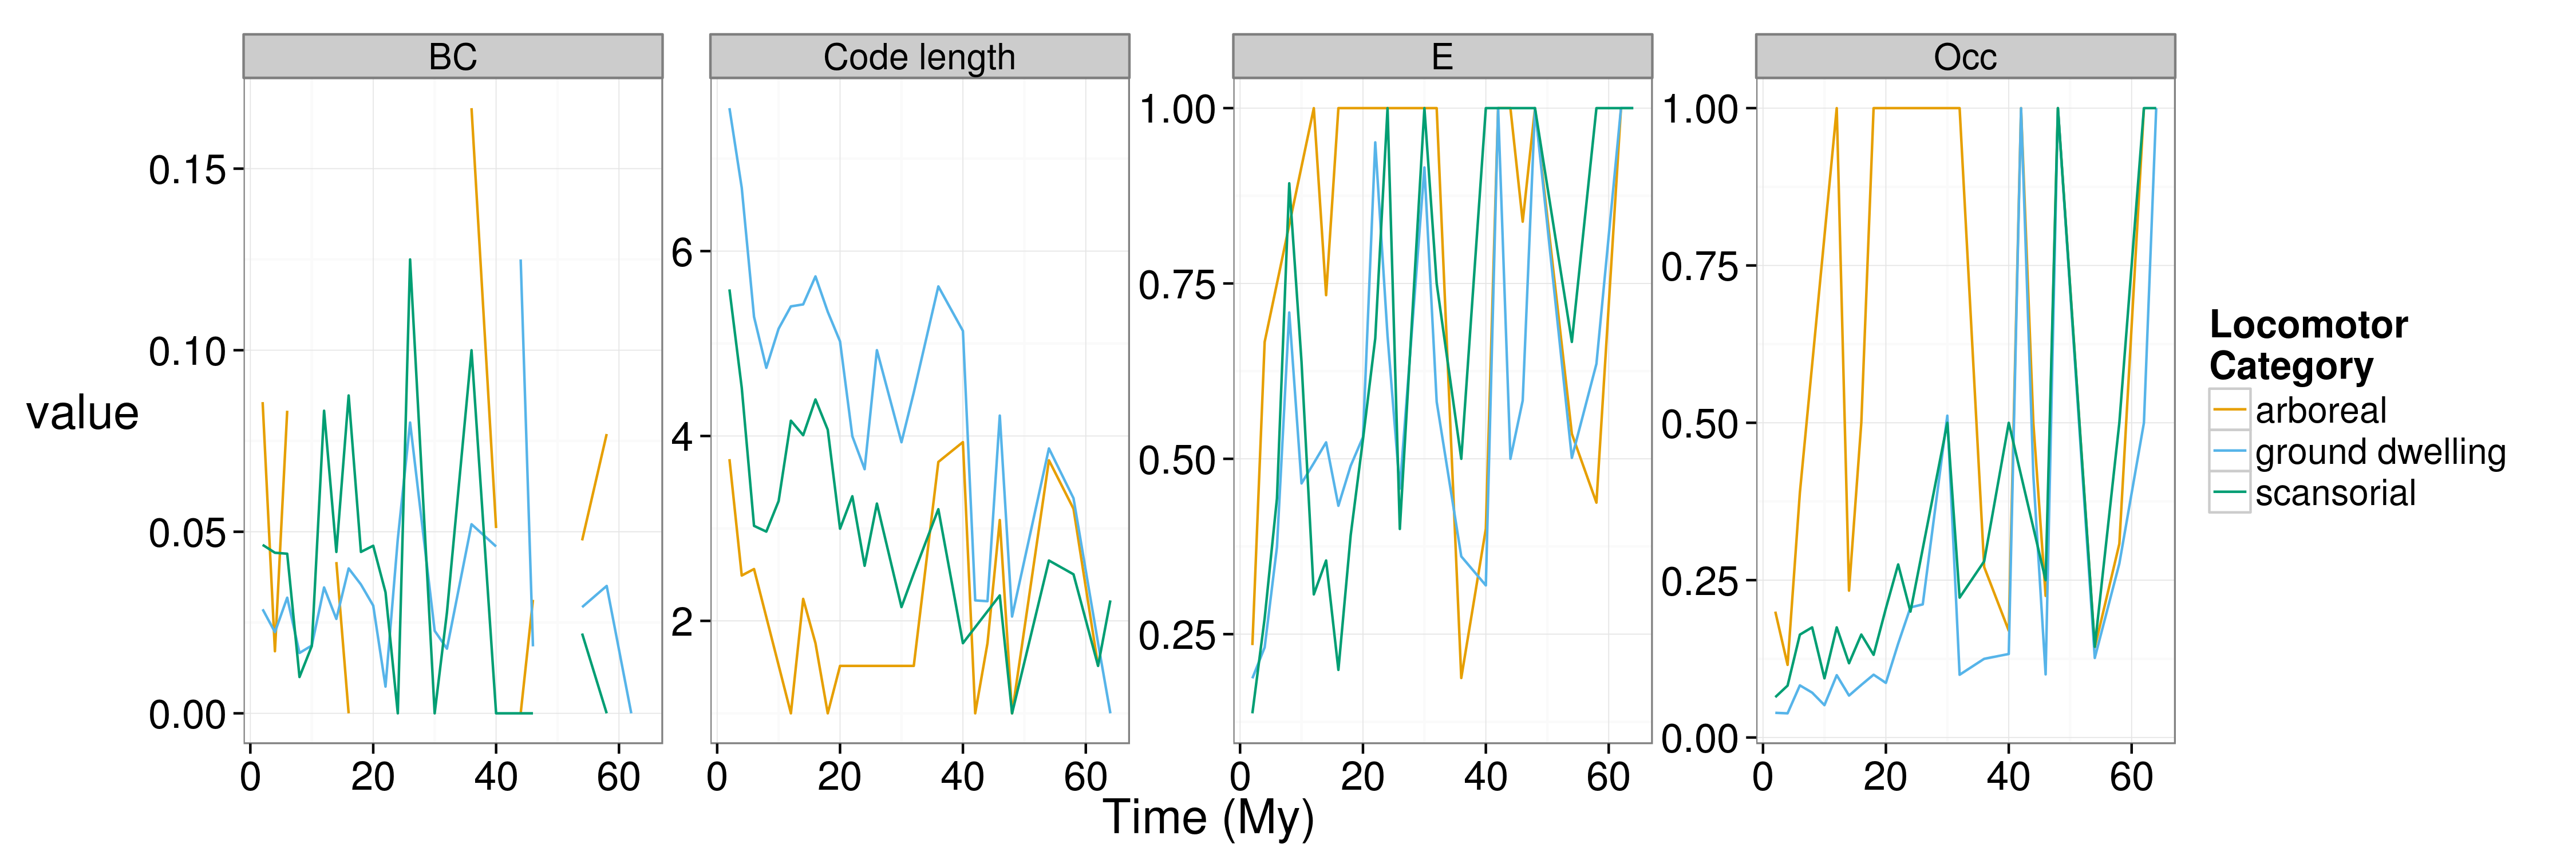
\includegraphics[width = \textwidth, keepaspectratio = true]{figure/er_lf}
      \label{subfig:loco_con_er}
    \end{subfigure}
  \end{center}
  \caption[Locomotor category based community connectedness]{Time series of summary statistics for biogeographic networks determined by locomotor category for North America (\subref{subfig:loco_con_na}) and Europe (\subref{subfig:loco_con_er}). The summary statistics are, clockwise from top left: biogeographic connectedness (BC), code length, average relative locality occupancy per taxon (Occ), and average relative number of endemic taxa per locality (E).} 
  \label{fig:loco_con}
\end{figure}

When taxa are separated by locomotor category, there is qualitatively less noise then is the case for by dietary category (Fig. \ref{fig:loco_con}). \(BC\) for North America has qualitative differences between each of the three categories (Fig. \ref{subfig:loco_con_na}). Arboreal taxa can only be measured for \(BC\) predominately during the Paleogene where there is no qualitative pattern beyond high variance. Scansorial taxa have a qualitative decline in volatility and was stationary during the Neogene. European values of \(BC\) were generally more volatile and very difficult to measure during the Paleogene because of the paucity of geographically spaced localities (Fig. \ref{subfig:loco_con_er}). Qualitatively, values of \(BC\) for scansorial taxa are more volatile than for ground dwelling taxa. 

For North American values of code length, there are a few clear qualitative patterns (Fig. \ref{subfig:loco_con_na}). Ground dwelling taxa have generally the highest code length values, followed by scansorial and arboreal taxa. Interestingly, all three of these categories have almost identical code length values until approximately 50 My. Following this, arboreal taxa have a qualitative decrease in code length, while scansorial taxa are qualitatively stationary with a slight decrease, and ground dwelling taxa have a slight increase though are mostly stationary. European code length values show a general increase during the entire Cenozoic, though this is mostly confined to scansorial and ground dwelling taxa (Fig. \ref{subfig:loco_con_er}).

The \(E\) series for North America demonstrates qualitatively distinct patterns for the three locomotor categories (Fig. \ref{subfig:loco_con_na}). \(E\) increases dramatically for arboreal taxa, has a moderate increase for scansorial taxa, and is qualitatively stationary for ground dwelling taxa during the Cenozoic. In comparison for Europe, values of \(E\) are generally high throughout the entire Cenozoic and vary with much greater volatility (Fig. \ref{subfig:loco_con_er}. Qualitatively there is a decrease in \(E\) for ground dwelling and scansorial taxa during the Neogene.

Values of \(Occ\) for both North America and Europe show respectively qualitatively similar patterns to patterns of \(E\), though are less volatile. \(Occ\) increases in North American arboreal taxa at approximately 40 My years ago while both scansorial and ground dwelling taxa are qualitatively stationary (Fig. \ref{subfig:loco_con_na}). The pattern of \(Occ\) for scansorial taxa appears to qualitatively be a more exaggerated version of the pattern for ground dwelling taxa. All three appear correlated during the earliest Cenozoic. As with \(E\), European patterns of \(Occ\) are volatile, particularity during the early Cenozoic (Fig. \ref{subfig:loco_con_er}). At approximately 40 My, patterns of \(Occ\) become less volatile and qualitatively decrease for ground dwelling and scansorial taxa. In comparison, \(Occ\) values for arboreal taxa become qualitatively much higher during the late Cenozoic with a massive decrease near the Recent.

These analyses will be greatly improved by varying locality ``size'', comparison with South American patterns, comparison of major orders, and other ideas stated above (Section \ref{sec:mamcommeth}). Additionally, quantitatively analysis of these patterns and what correlations might exist, especially in a phylogenetic context, are necessary in order to better understand what processes might dominate and when.

\clearpage

\section{Synthesis of proposed research} \label{sec:synth}
Underlying all of the above is a foundational question in paleobiology: why do certain taxa go extinct while others do not? In the context of evolutionary paleoecology, this question can be rephrased as ``how do the set of all biotic--biotic and biotic--abiotic interactions a taxon experiences over time (i.e. adaptive zone \citealp{Simpson1944}) affect extinction risk?'' Related to this is the Law of Constant Extinction which states that extinction risk for a given adaptive zone is taxon--age independent \citep{VanValen1973}. It is asserted that the Law of Constant Extinction only holds during periods of relatively constant environment, even though this was not the context for the initial observation \citep{Liow2007b,VanValen1973}, which can be interpreted as the set of dominant non-organism mediated processes do not fluctuate or fluctuate in a known manner. By understanding which non-organism mediated processes may be shaping the environment (set of all possible biotic and abiotic interactors) and how they change over time and phrasing analysis of extinction in this context, it may be possible to ``test'' the Law of Constant Extinction.

The two studies proposed above (Sections \ref{sec:bracsurv} and \ref{sec:mamsurv}) investigate how organismal traits potentially related to environmental preference affect extinction rate. In effect, these traits may determine the ``bounds'' of a taxon's adaptive zone by limiting the total set of interactions to just those for which the taxon is adapted. The other two proposed studies (Sections \ref{sec:braccom} and \ref{sec:mamcom}) aim to estimate what non-organism mediated processes (global, regional, and/or local) may be dominate in shaping the environment and the related set of adaptive zones. Between these studies, as well the use of two disparate groups, it should be possible to determine when, what, and if certain variables matter for survival and, potentially, how they matter. 

\clearpage

\section{Timeline}

Spring/Summer 2014
\begin{itemize}
  \item Evolution Meeting: preliminary brachiopod survival results
  \item South American fossil mammal data from American Museum of Natural History collections
\end{itemize}

Fall 2014/Winter 2015
\begin{itemize}
  \item GSA: survivorship simulation for anagenesis and sampling
  \item Doctoral Dissertation Improvement Grant
\end{itemize}

Spring/Summer 2015
\begin{itemize}
  \item Evolution Meeting: mammalian survivorship analysis for North America and Europe
  \item write and submit survivorship simulation paper
  \item possible South American fossil mammal data from American Museum of Natural History collections
\end{itemize}

Fall 2015/Winter 2016
\begin{itemize}
  \item SVP: mammalian biogeographic connectedness
  \item write and submit mammal connectedness paper
\end{itemize}

Spring/Summer 2016
\begin{itemize}
  \item Evolution Meeting: brachiopod survival analysis
  \item write and submit brachiopod survival paper
\end{itemize}

Fall 2016/Winter 2017
\begin{itemize}
  \item GSA: brachiopod community connectedness
  \item write and submit mammal survival paper
\end{itemize}

Spring/Summer 2017
\begin{itemize}
  \item Evolution Meeting: survival and communities together
  \item write and submit brachiopod community paper
  \item write and review/philosophy paper
  \item \textbf{Defend}
\end{itemize}


\clearpage
\bibliographystyle{abbrvnat}
\bibliography{proposal}


\clearpage


\appendix

\section{Permian lithology and paleoenvironment} \label{sec:env_app}
Lithological and paleoenvironmental assignments avaliable in the PBDB can be poorly resolved or missing in the case of environment. Because these assignments are critical in the proposed study of brachiopod survival and distribution (Section \ref{sec:brac}), it is necessary to improve these values with more precise information avaliable in the paleontological and geological literature.

The geological unit reference guide on from Geosciences Australia (\url{http:/www.ga.goc.au/}), the lithological information for many of the brachiopod occurrences can be improved and made more precise (Table \ref{tab:form_lith}). The lithological assignments below are based on the order with which rock types are named in the lithological description of a geological unit. These were extracted automatically using a very simple algorithm. While more than two rock types may be listed for a geological unit, only the first two are reported below. These formations represent 3533 of 5737 (61\%) total occurrences across all of Australia.

Below is a set of representative PBDB assignments and my improvements, focused primarily on paleoenvironmental reconstruction (Table \ref{tab:paleoenv}). These assignments are very preliminary and based only on a few key papers and associated maps \citep{Percival2012,Fielding2006,Hawley1995}. There are a total of 5737 Permian Australian brachiopod occurrences in the PBDB, from both Eastern and Western Australia. Within is, there are 4711 occurrences that are not from Western Australia. The geological units listed in Table \ref{tab:paleoenv}, which are from Eastern Australia, account for 289 of these occurrences which is about 5\% of the total samples or 6\% of the east Australian samples.

% latex table generated in R 3.0.2 by xtable 1.7-1 package
% Mon Mar  3 17:23:32 2014
\begin{table}[ht]
\centering
\begin{tabular}{lllll}
  \hline
geological unit & PDBD lithology 1 & PBDB lithology 2 & my lithology 1 & my lithology 2 \\ 
  \hline
Aldebaran Sandstone & sandstone &  & conglomerate & siltstone \\ 
  Allandale Formation & siliciclastic &  & conglomerate & sandstone \\ 
  Alum Rock Conglomerate Bondonga/Pikedale/Silver Spur and Terrica beds & siliciclastic &  & tuff & limestone \\ 
  Baker Formation & siltstone &  & siltstone & quartz \\ 
  Bakers Blue Granite & siltstone &  & granodiorite &  \\ 
  Bakers Creek Diorite & siltstone &  & diorite & quartzbiotite \\ 
  Bakers Creek Suite & siltstone &  & gabbros & diorites \\ 
  Bakerville Granodiorite & siltstone &  & granodiorite &  \\ 
  Barfield Formation & sandstone &  & tuff & conglomerate \\ 
  Beekeeper Formation & not reported &  & carbonatesiliciclastic & carbonatesiliciclastic \\ 
  Berserker Group & siliciclastic &  & conglomerates & breccia \\ 
  Billidee Formation & sandstone &  & siltstone & shale \\ 
  Black Alley Shale & shale &  & shale & siltstone \\ 
  Black Jack Granodiorite & siliciclastic &  & granite & granodiorite \\ 
  Black Jack Group & siliciclastic &  & sandstone &  \\ 
  Blenheim Formation & sandstone &  & sandstone & coquinite \\ 
  Broughton River Granodiorite & sandstone &  & granodiorite & granite \\ 
  Broughton River Suite & sandstone &  & granodiorite &  \\ 
  Buffel Formation & siliciclastic &  & limestone & limestone \\ 
  Bulgadoo Shale & shale &  & shale & siltstone \\ 
  Burnett Formation & sandstone &  & arenite & siltstone \\ 
  Callytharra Formation &  &  & calcarenite & conglomerate \\ 
  Carmila beds & siliciclastic &  & siltstone & basalt \\ 
  Carolyn Formation & sandstone & claystone & sandstone & sandstone \\ 
  Carrandibby Formation & siliciclastic &  & claystone & siltstone \\ 
  Catherine Sandstone & sandstone &  & siltstone & mudstone \\ 
  Cattle Creek Formation & siliciclastic &  & mudstone & quartzose \\ 
  Condamine beds & mudstone &  & conglomerate & tuff \\ 
  Coolkilya Sandstone & sandstone &  & quartz & siltstone \\ 
  Coyrie Formation & siliciclastic &  & shale & siltstone \\ 
  Crocker Well Suite & siliciclastic &  & granodiorite &  \\ 
  Cundlego Formation &  &  & siltstone & shale \\ 
  Darlington Limestone & limestone &  & limestones & calcirudites \\ 
  Eight Mile Creek beds & siliciclastic &  & conglomerate & sandstone \\ 
  Eight Mile Creek Granite & siliciclastic &  & granite &  \\ 
  Eight Mile Creek Granodiorite & siliciclastic &  & granite &  \\ 
  Flat Top Diorite & sandstone &  & diorite & diorite \\ 
  Flat Top Formation & sandstone &  & tuff & sandy \\ 
  Freitag Formation & sandstone &  & sandstone & sandstone \\ 
  Gilgurry Mudstone & mudstone &  & mudstone & sandstone \\ 
  Glencoe Gabbro & mudstone &  & gabbro & gabbro \\ 
  Glencoe Limestone Member & mudstone &  & limestone &  \\ 
  Glenmore Creek Granite & siliciclastic &  & monzogranite &  \\ 
  Gray Creek Complex & siltstone &  & metagabbro &  \\ 
  Hardman Formation & sandstone &  & sandstone & limestone \\ 
  Hickman Creek Granite & siliciclastic &  & monzogranite &  \\ 
  High Cliff Sandstone & sandstone &  & siltstone & shale \\ 
  Holmwood Shale & siliciclastic &  & limestone & shale \\ 
  Ingelara Formation & siliciclastic &  & sandy & siltstone \\ 
  Ingliston Granite & siliciclastic &  & granite &  \\ 
  Lakes Creek Formation & not reported &  & volcanics & sandstones \\ 
  Lizzie Creek Volcanic Group/Mount Wickham Rhyolite & sandstone &  & andesite & rhyolite \\ 
  Lochinvar Formation & limestone &  & basalt & siltstone \\ 
  Manning Group & siliciclastic &  & mudstone & conglomerate \\ 
  Maria Formation & siliciclastic &  & mudstone & shale \\ 
  Maria Island Granite & siliciclastic &  & granite &  \\ 
  Marra Creek Formation & siliciclastic &  & sandy & carbonate \\ 
  Marra Formation & siliciclastic &  & sandstone & siltstone \\ 
  Marrangaroo Conglomerate & siliciclastic &  & sandstone & conglomerate \\ 
  Marrar Dyke & siliciclastic &  & monzogabbro &  \\ 
  Mistletoe Granite & siliciclastic &  & granite &  \\ 
  Moonlight Valley Tillite & sandstone &  & conglomerate & sandstone \\ 
  Mooraback beds & siliciclastic &  & sandstone & siltstone \\ 
  Mount Poole Monzogranite & siliciclastic &  & monzogranite &  \\ 
  Muggleton Formation & siliciclastic &  & shale & quartzose \\ 
  Mulbring Siltstone & sandstone &  & claystone & sandstone \\ 
  Muree Sandstone & siltstone &  & sandstone & conglomerate \\ 
  Narayen beds & siliciclastic &  & conglomerate & siltstone \\ 
  Nowra Sandstone & sandstone &  & conglomerate & quartzose \\ 
  Oxtrack Formation & siltstone &  & chert & siltstone \\ 
  Peawaddy Formation & siliciclastic &  & siltstone & siltstone \\ 
  Poole Sandstone & siliciclastic &  & conglomerate & quartzose \\ 
  Porcupine Creek Granodiorite & siliciclastic &  & granodiorite &  \\ 
  Porcupine Creek rhyolite & siliciclastic &  & ignimbrite &  \\ 
  Porcupine Formation & siliciclastic &  & conglomerate & sandstone \\ 
  Quinnanie Shale & shale &  & shale & siltstone \\ 
  Rammutt Formation & siliciclastic &  & mudstone & basaltic \\ 
  Rhyolite Range beds & siliciclastic &  & sandstone & siltstone \\ 
  Risdon Stud Formation & sandstone &  & tuff & arenite \\ 
  Rutherford Formation & siliciclastic &  & marl & sandstone \\ 
  Silver Spur beds & siliciclastic &  & conglomerate & mudstone \\ 
  Snapper Point Formation/Wandrawandian Siltstone & siltstone &  & sandstone & siltstone \\ 
  South Curra Limestone & limestone &  & grainstone & calcilutite \\ 
  Tamby Creek Formation & siliciclastic &  & andesite & breccia \\ 
  Tomago Coal Measures & siliciclastic &  & tuff & siltstone \\ 
  Towgon Grange Tonalite & mudstone &  & granodiorite & diorite \\ 
  Wandagee Formation &  &  & siltstone & quartz \\ 
  Wandrawandian Siltstone & siltstone &  & siltstone & quartzlithic \\ 
  Watermark Formation & siliciclastic &  & siltstone & claystone \\ 
  Werrie Basalt & siliciclastic &  & basaltic & tuffs \\ 
  Yessabah Limestone & limestone &  & limestone & mudstone \\ 
   \hline
\end{tabular}
\label{tab:form_lith}
\end{table}
  %tab:form_lith

\begin{sidewaystable}[ht]\footnotesize
  \centering
  \begin{tabular}{l l l l l l l}
    \hline
    geological unit & PBDB lithology 1 & PBDB paleoenvironment & my lithology 1 & my lithology 2 & my paleoenvironment 1 & my paleoenvironment 2 \\ 
    \hline
    Mulbring & sandstone & marine indet & siltstone & sandstone & marine shelf &  \\ 
    Muree & siltstone & coastal indet & sandstone & conglomerate & alluvial fan & fan delta \\ 
    Branxton & siliciclastic & coastal indet & conglomerate & sandstone & fan delta & delta plain \\ 
    Farley & siliciclastic & marine indet & siltstone & sandstone & delta plain & delta front \\ 
    Rutherford & siliciclastic & coastal indet & siltstone & mudstone & delta front & marine shelf \\ 
    Allandale & siliciclastic & coastal indet & conglomerate & sandstone & sublittoral strand & marine shelf \\ 
    Lochinvar & limestone & marine indet & basalt & siltstone & sublittoral strand & marine shelf \\ 
    Snapper Point & sandstone & shoreface & sandstone & conglomerate & fluvial coastal & nearshore marine \\ 
    Berry & sandstone & marine indet & siltstone & shale & offshore marine &  \\ 
    Nowra & sandstone & coastal indet & sandstone &  & nearshore marine & coastal \\ 
    Wandrawandian & siltstone & offshore & siltstone & sandstone & offshore marine &  \\ 
    Wasp Head & sandstone & shoreface &  &  & alluvial valley fill & nearshore marine \\ 
    \hline
  \end{tabular}
  \caption[Improvements to PBDB geological information]{Australian geological units included in the study of brachiopod survival and distribution (Section \ref{sec:brac}). Both PBDB assignments and those sourced from the literature are included. Improvements are obvious, especially in regards to paleoenvironmental reconstruction.}
  \label{tab:paleoenv}
\end{sidewaystable}


\end{document}
